\subsection{Spielbasis}

%\begin{figure}[h]
%	\centering
%  	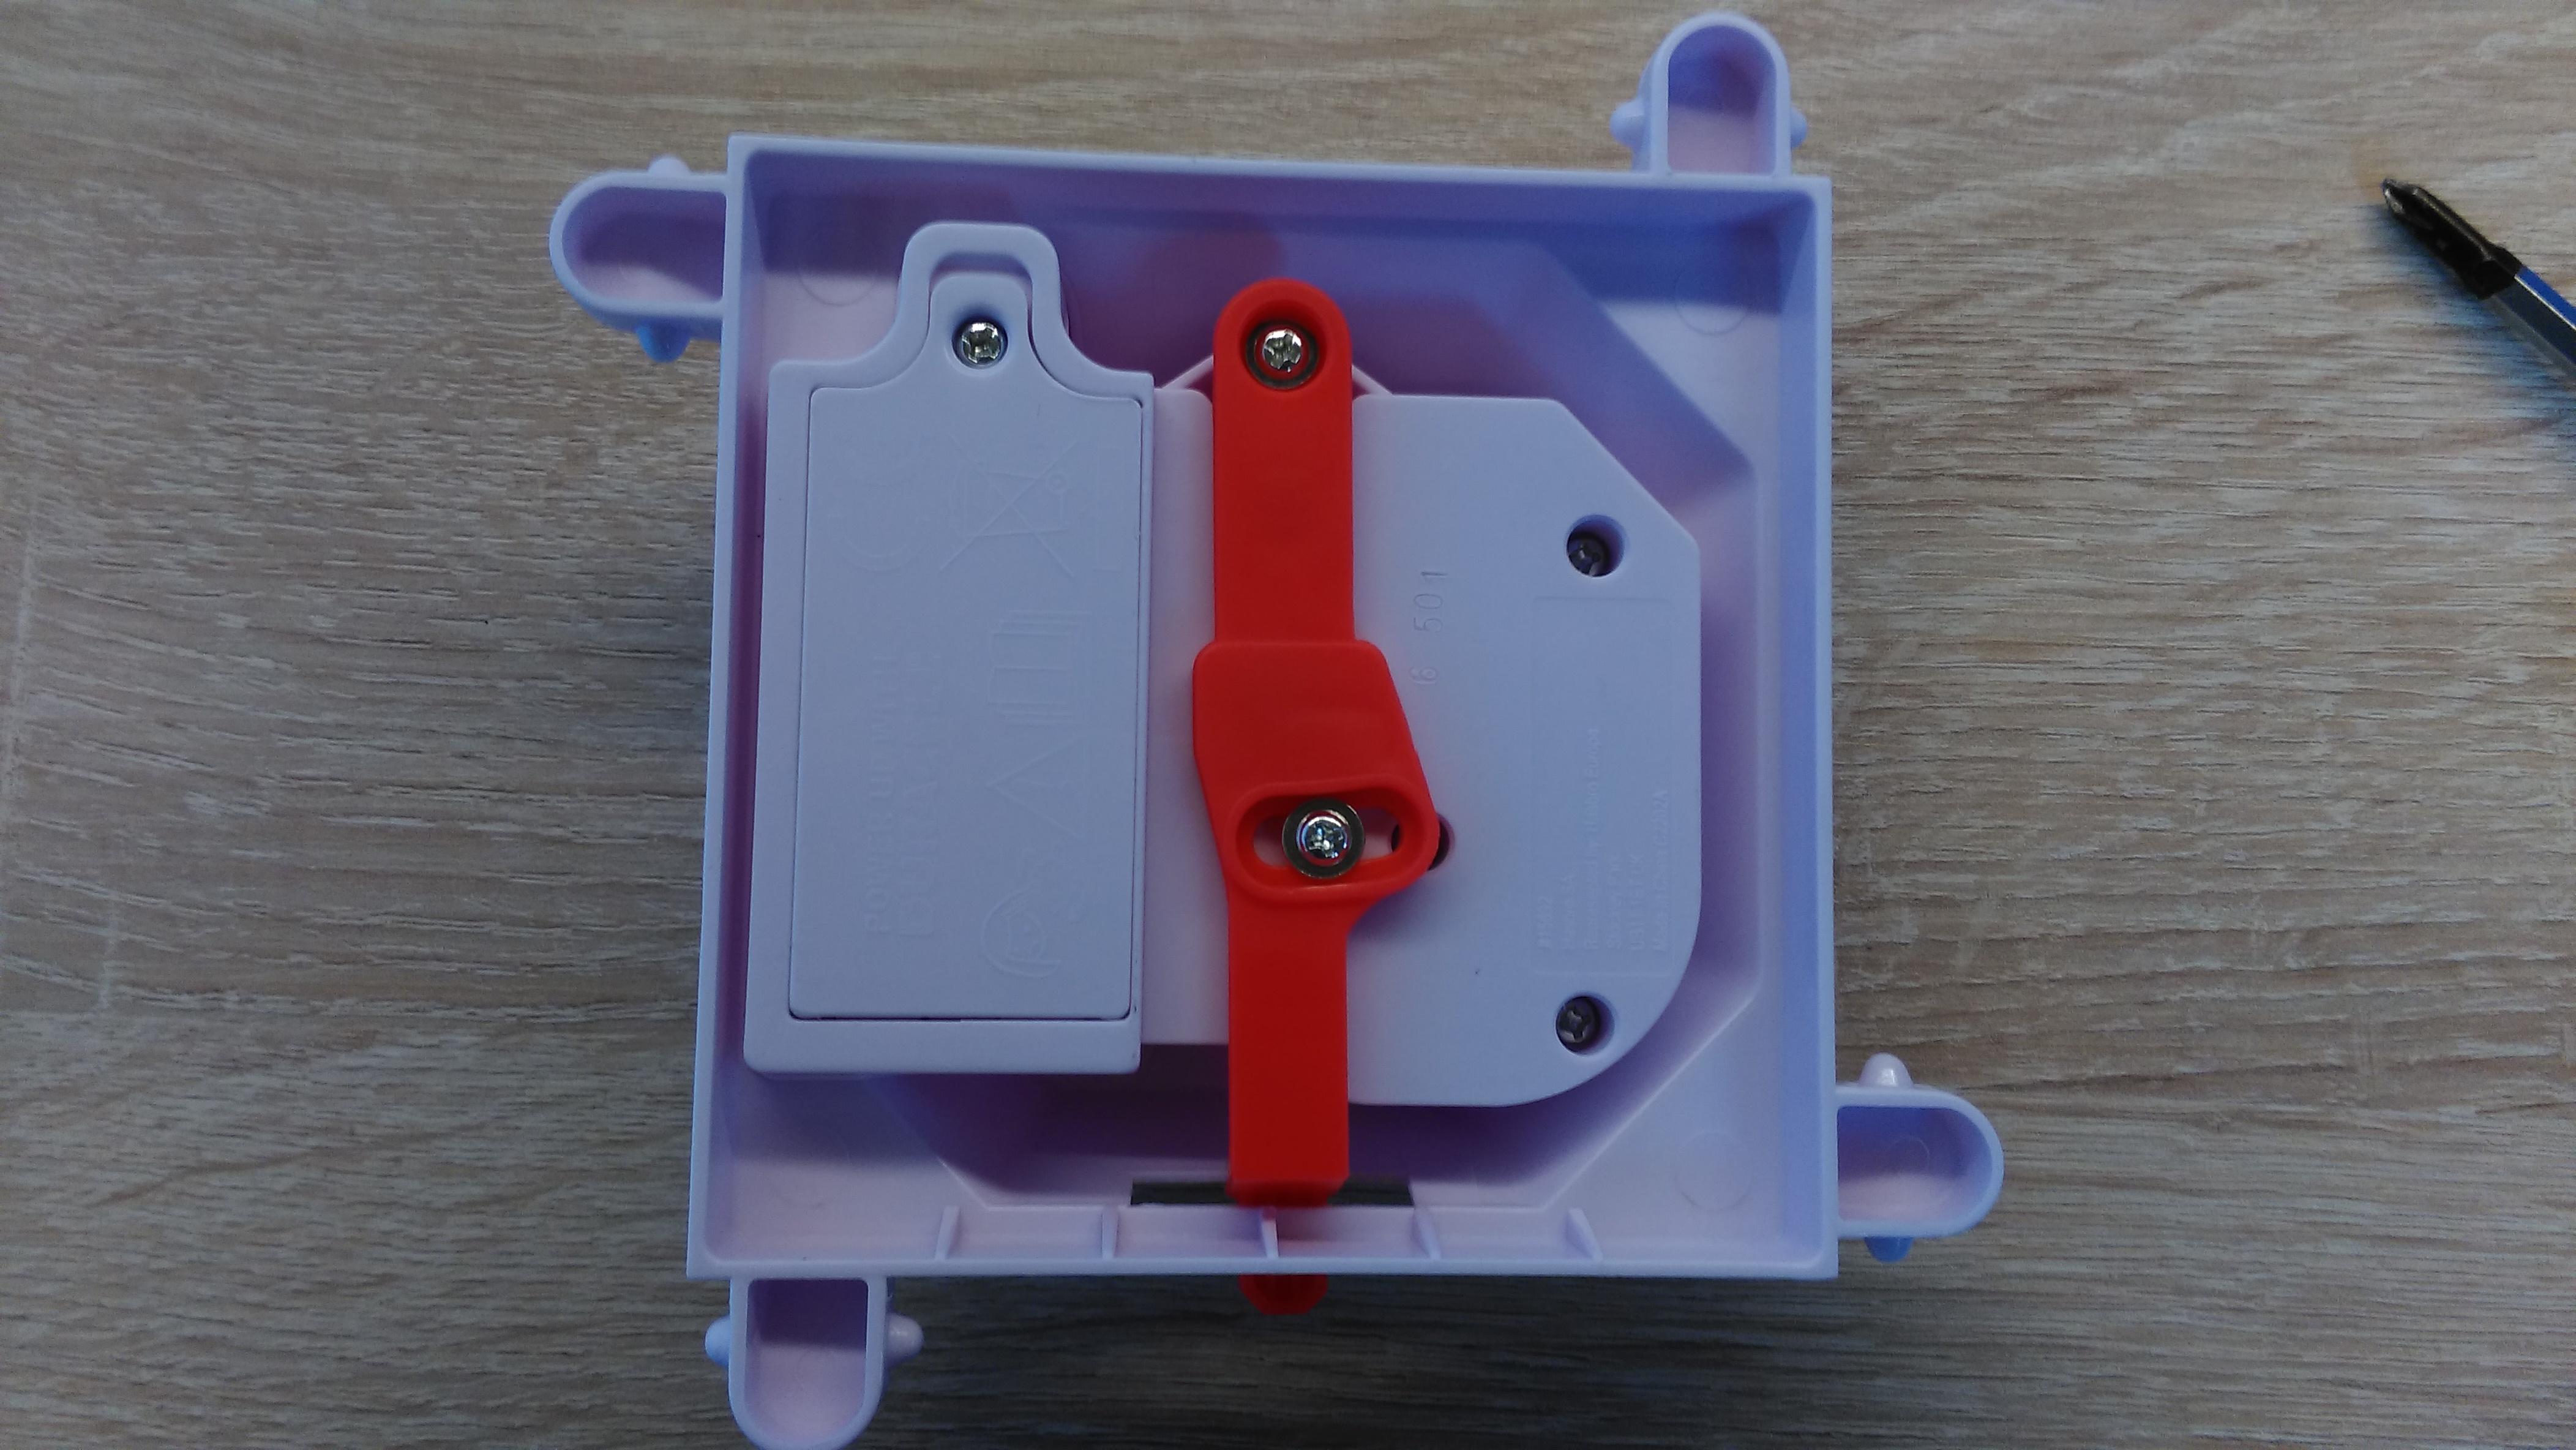
\includegraphics[width=0.7\textwidth]{pictures/loolou_001.jpg}
%	\caption{Spielbasis - Unterseite}
%	\label{fig1}
%\end{figure}

Als erstes widmen wir uns der Spielbasis, zu sehen in Abbildung ~\ref{fig2}. \\
Dazu entfernen wir als erstes die 7 Schrauben an der Unterseite. \\
Die ersten 5 Schrauben sind mit blo"sem Auge von aussen sichtbar. Die letzten zwei Schrauben sind nach dem "offnen des Batteriefaches zu sehen.  

\vspace{1cm}
\begin{figure}[!ht]
	\centering
  	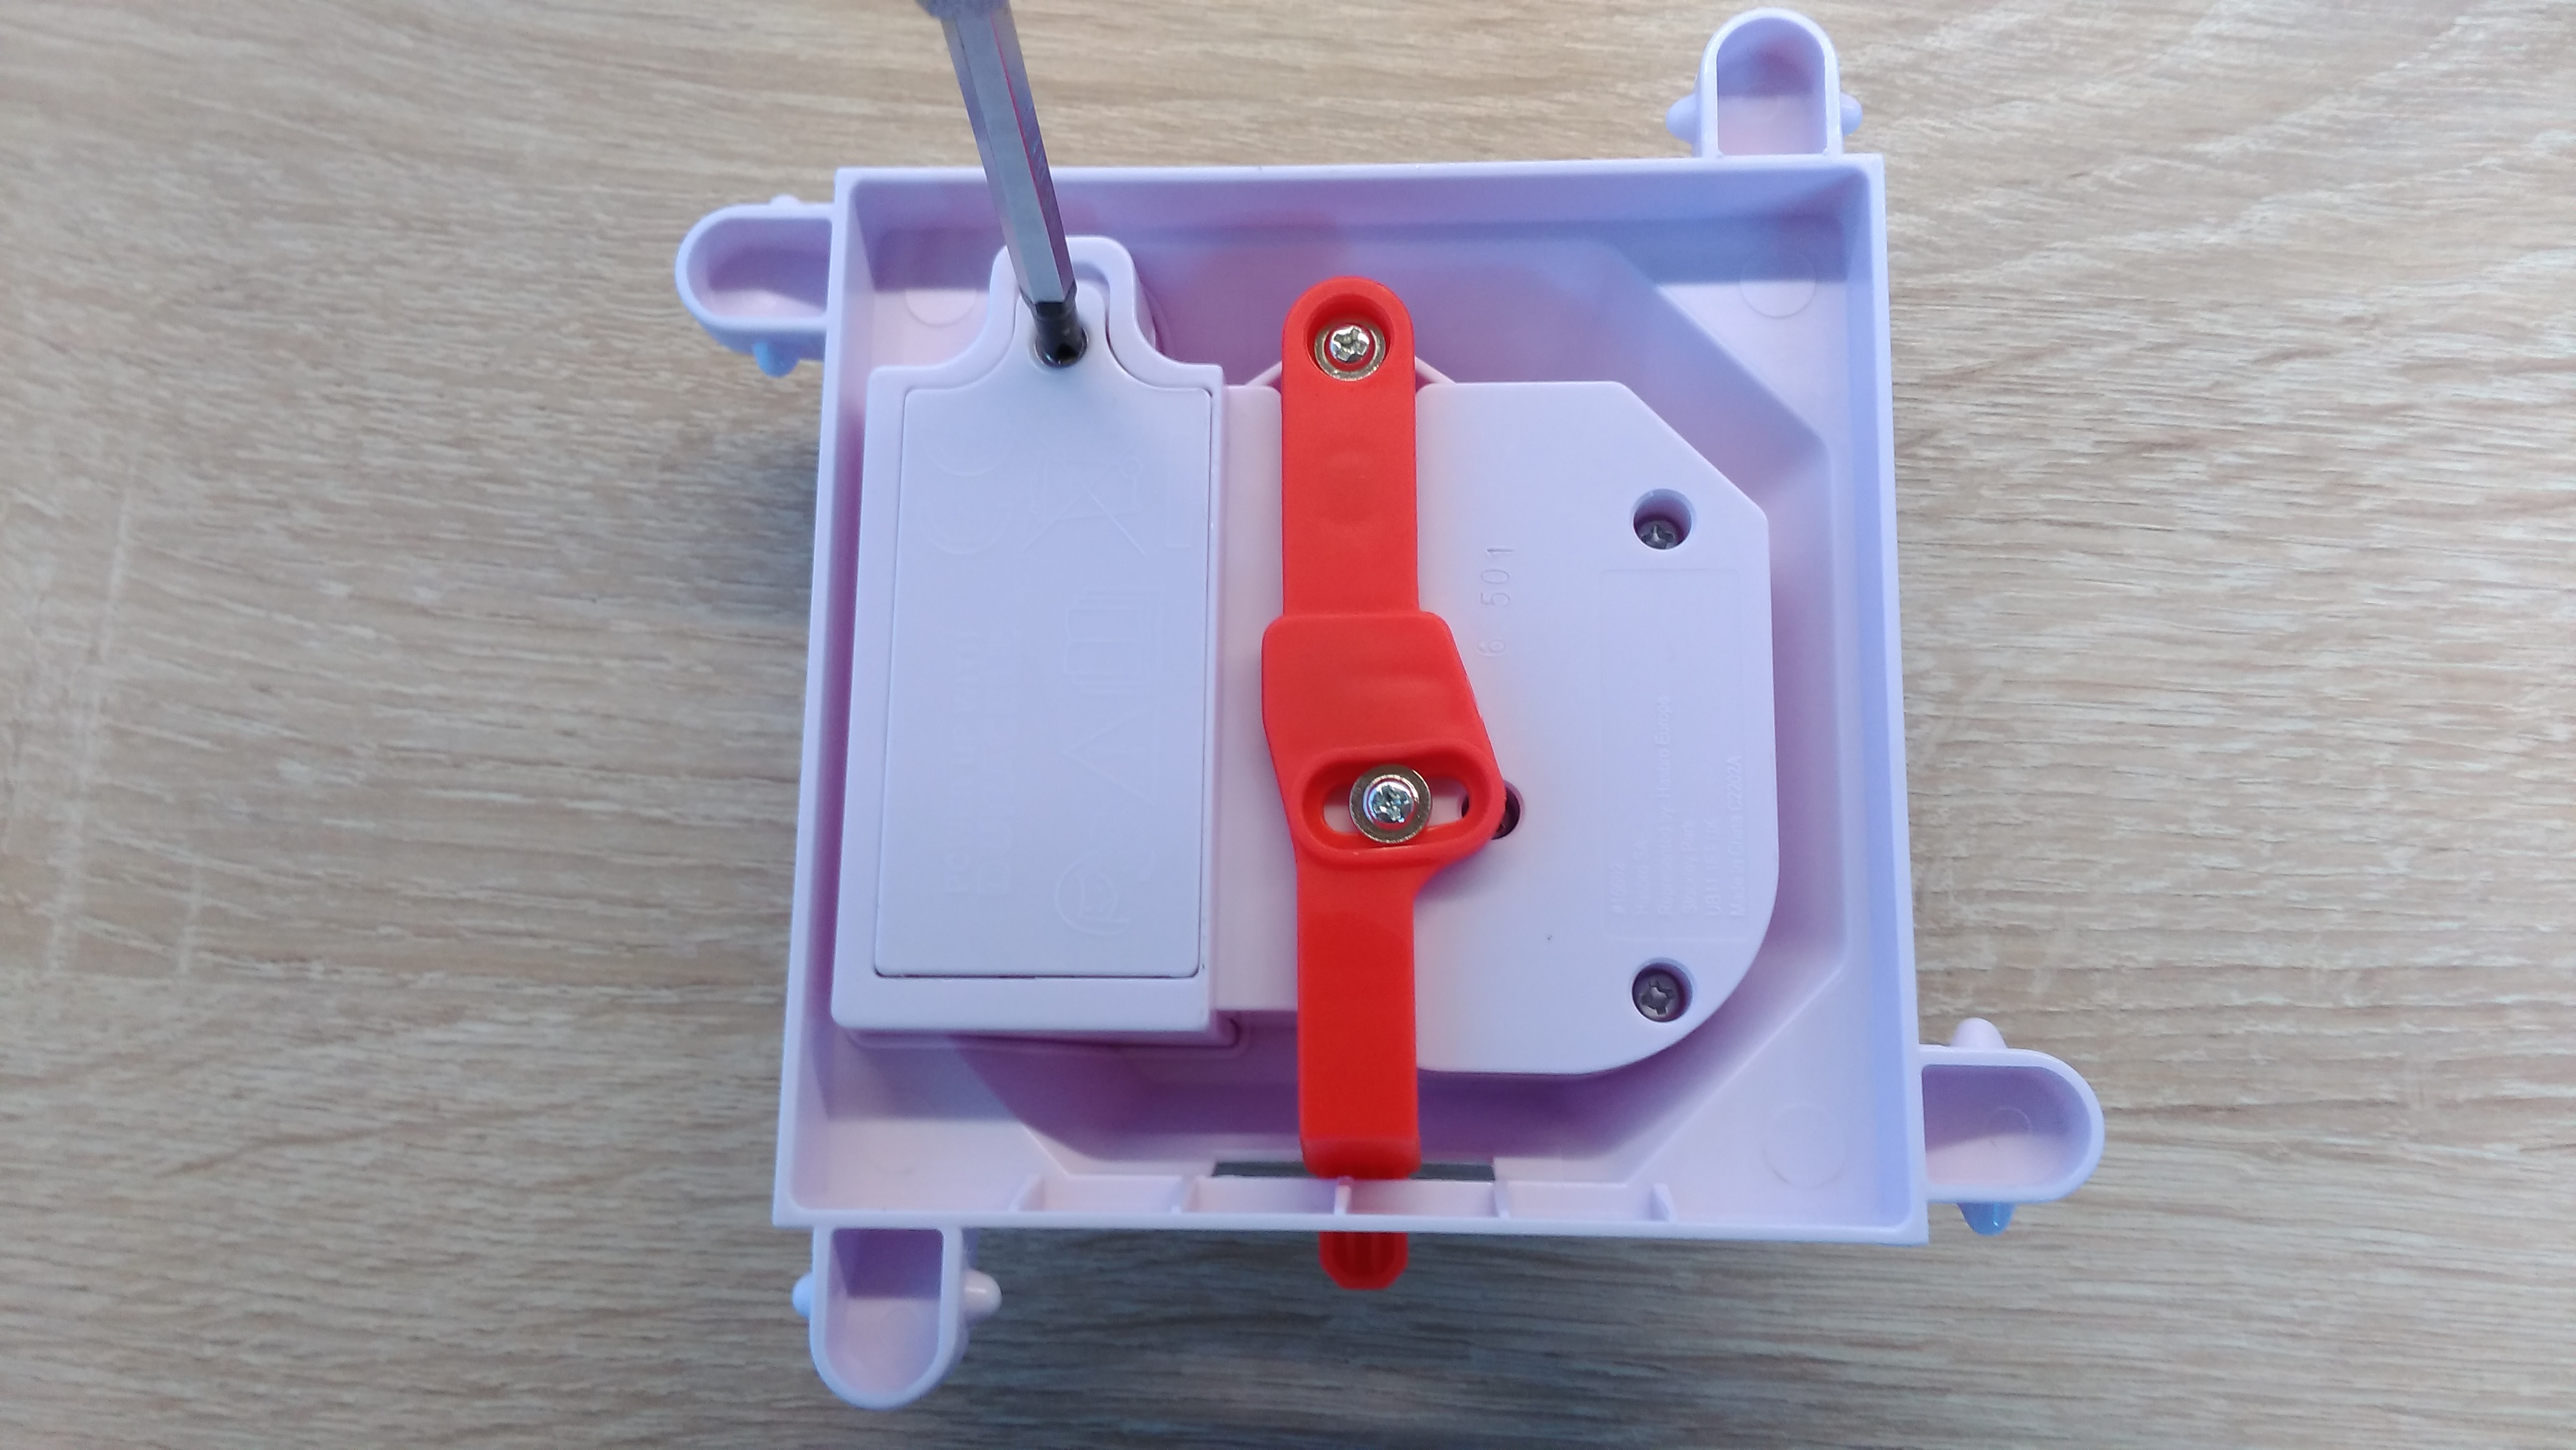
\includegraphics[width=0.7\textwidth]{pictures/loolou_002.jpg}
	\caption{Spielbasis - Unterseite aufschrauben}
	\label{fig2}
\end{figure}
\vspace{0.5cm}

Abbildung ~\ref{fig3} zeigt die Spielebasis nach dem entfernen der 7 Schrauben. 

\vspace{1cm}
\begin{figure}[!ht]
	\centering
  	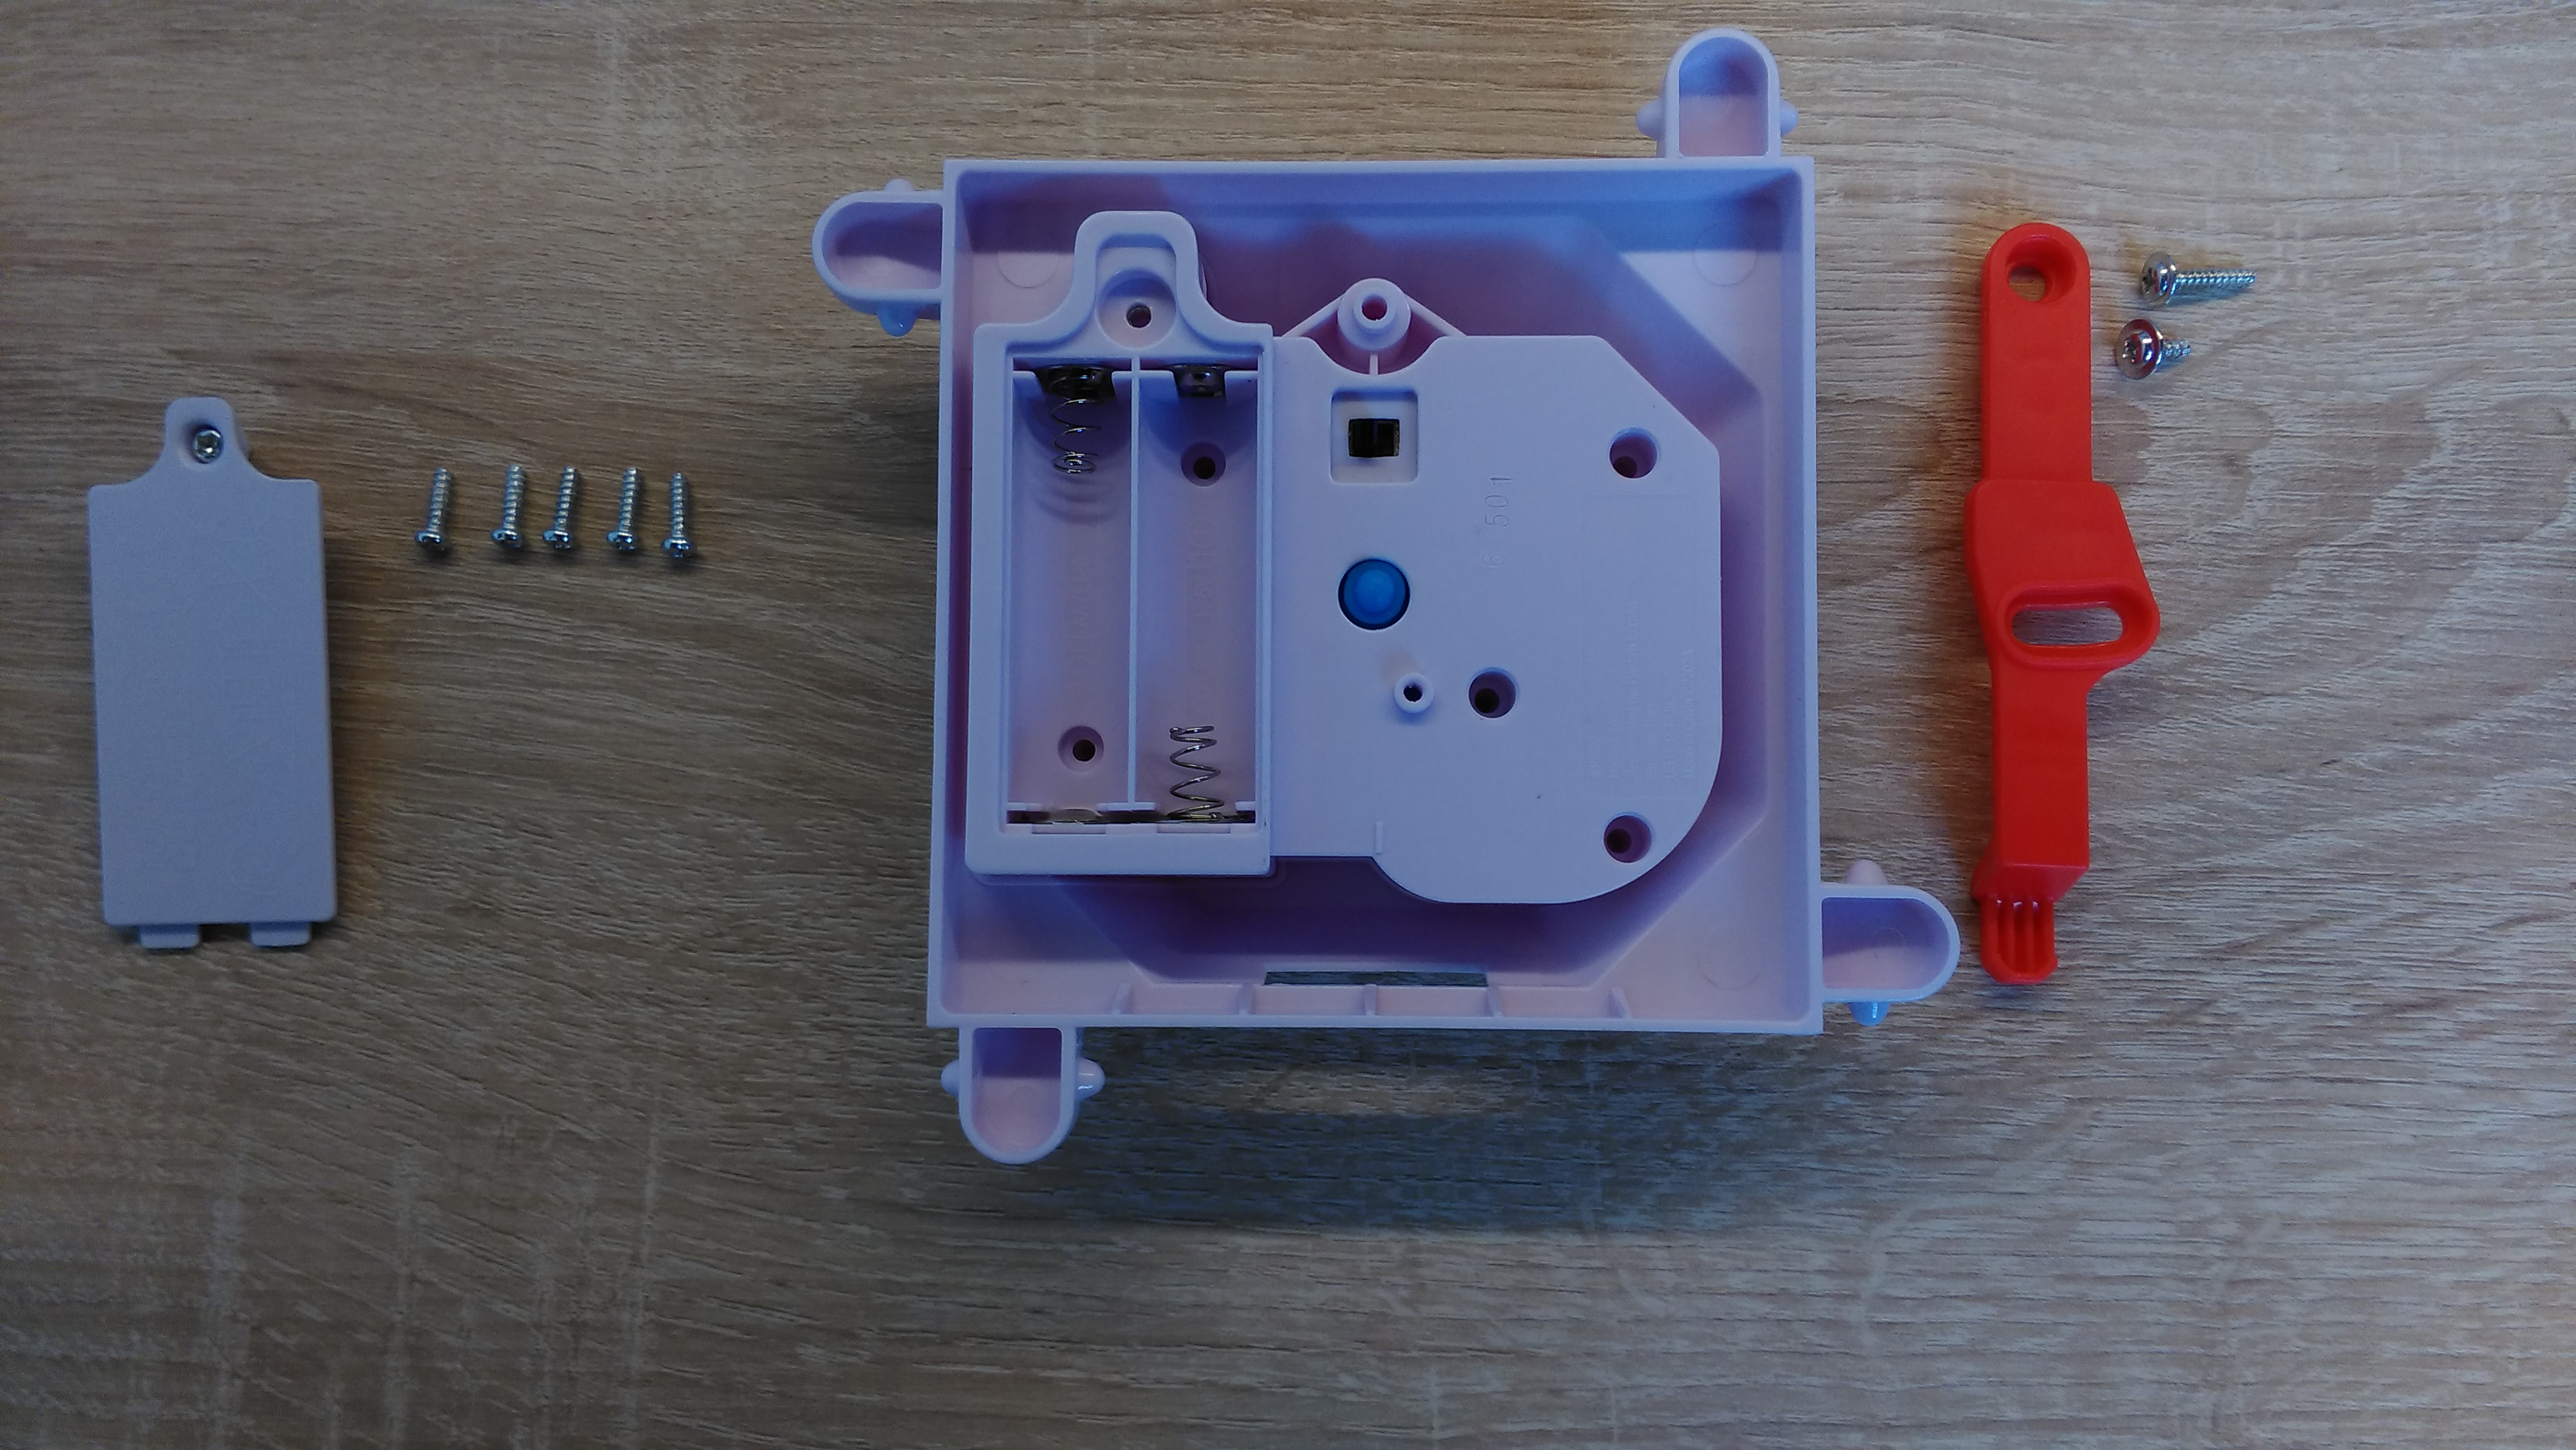
\includegraphics[width=0.7\textwidth]{pictures/loolou_003.jpg}
	\caption{Spielbasis - ge"offnet}
	\label{fig3}
\end{figure}
\vspace{0.5cm}

Anschlie"send muss die Spielbasis ge"offnet werden. Dazu zieht man das Innenteil der Spielbasis heraus.
Zu sehen ist nun das Getriebe, der Motor und der Stromschalter (siehe Abbildung ~\ref{fig4} und ~\ref{fig5}). 

\vspace{1cm}
\begin{figure}[!ht]
	\centering
  	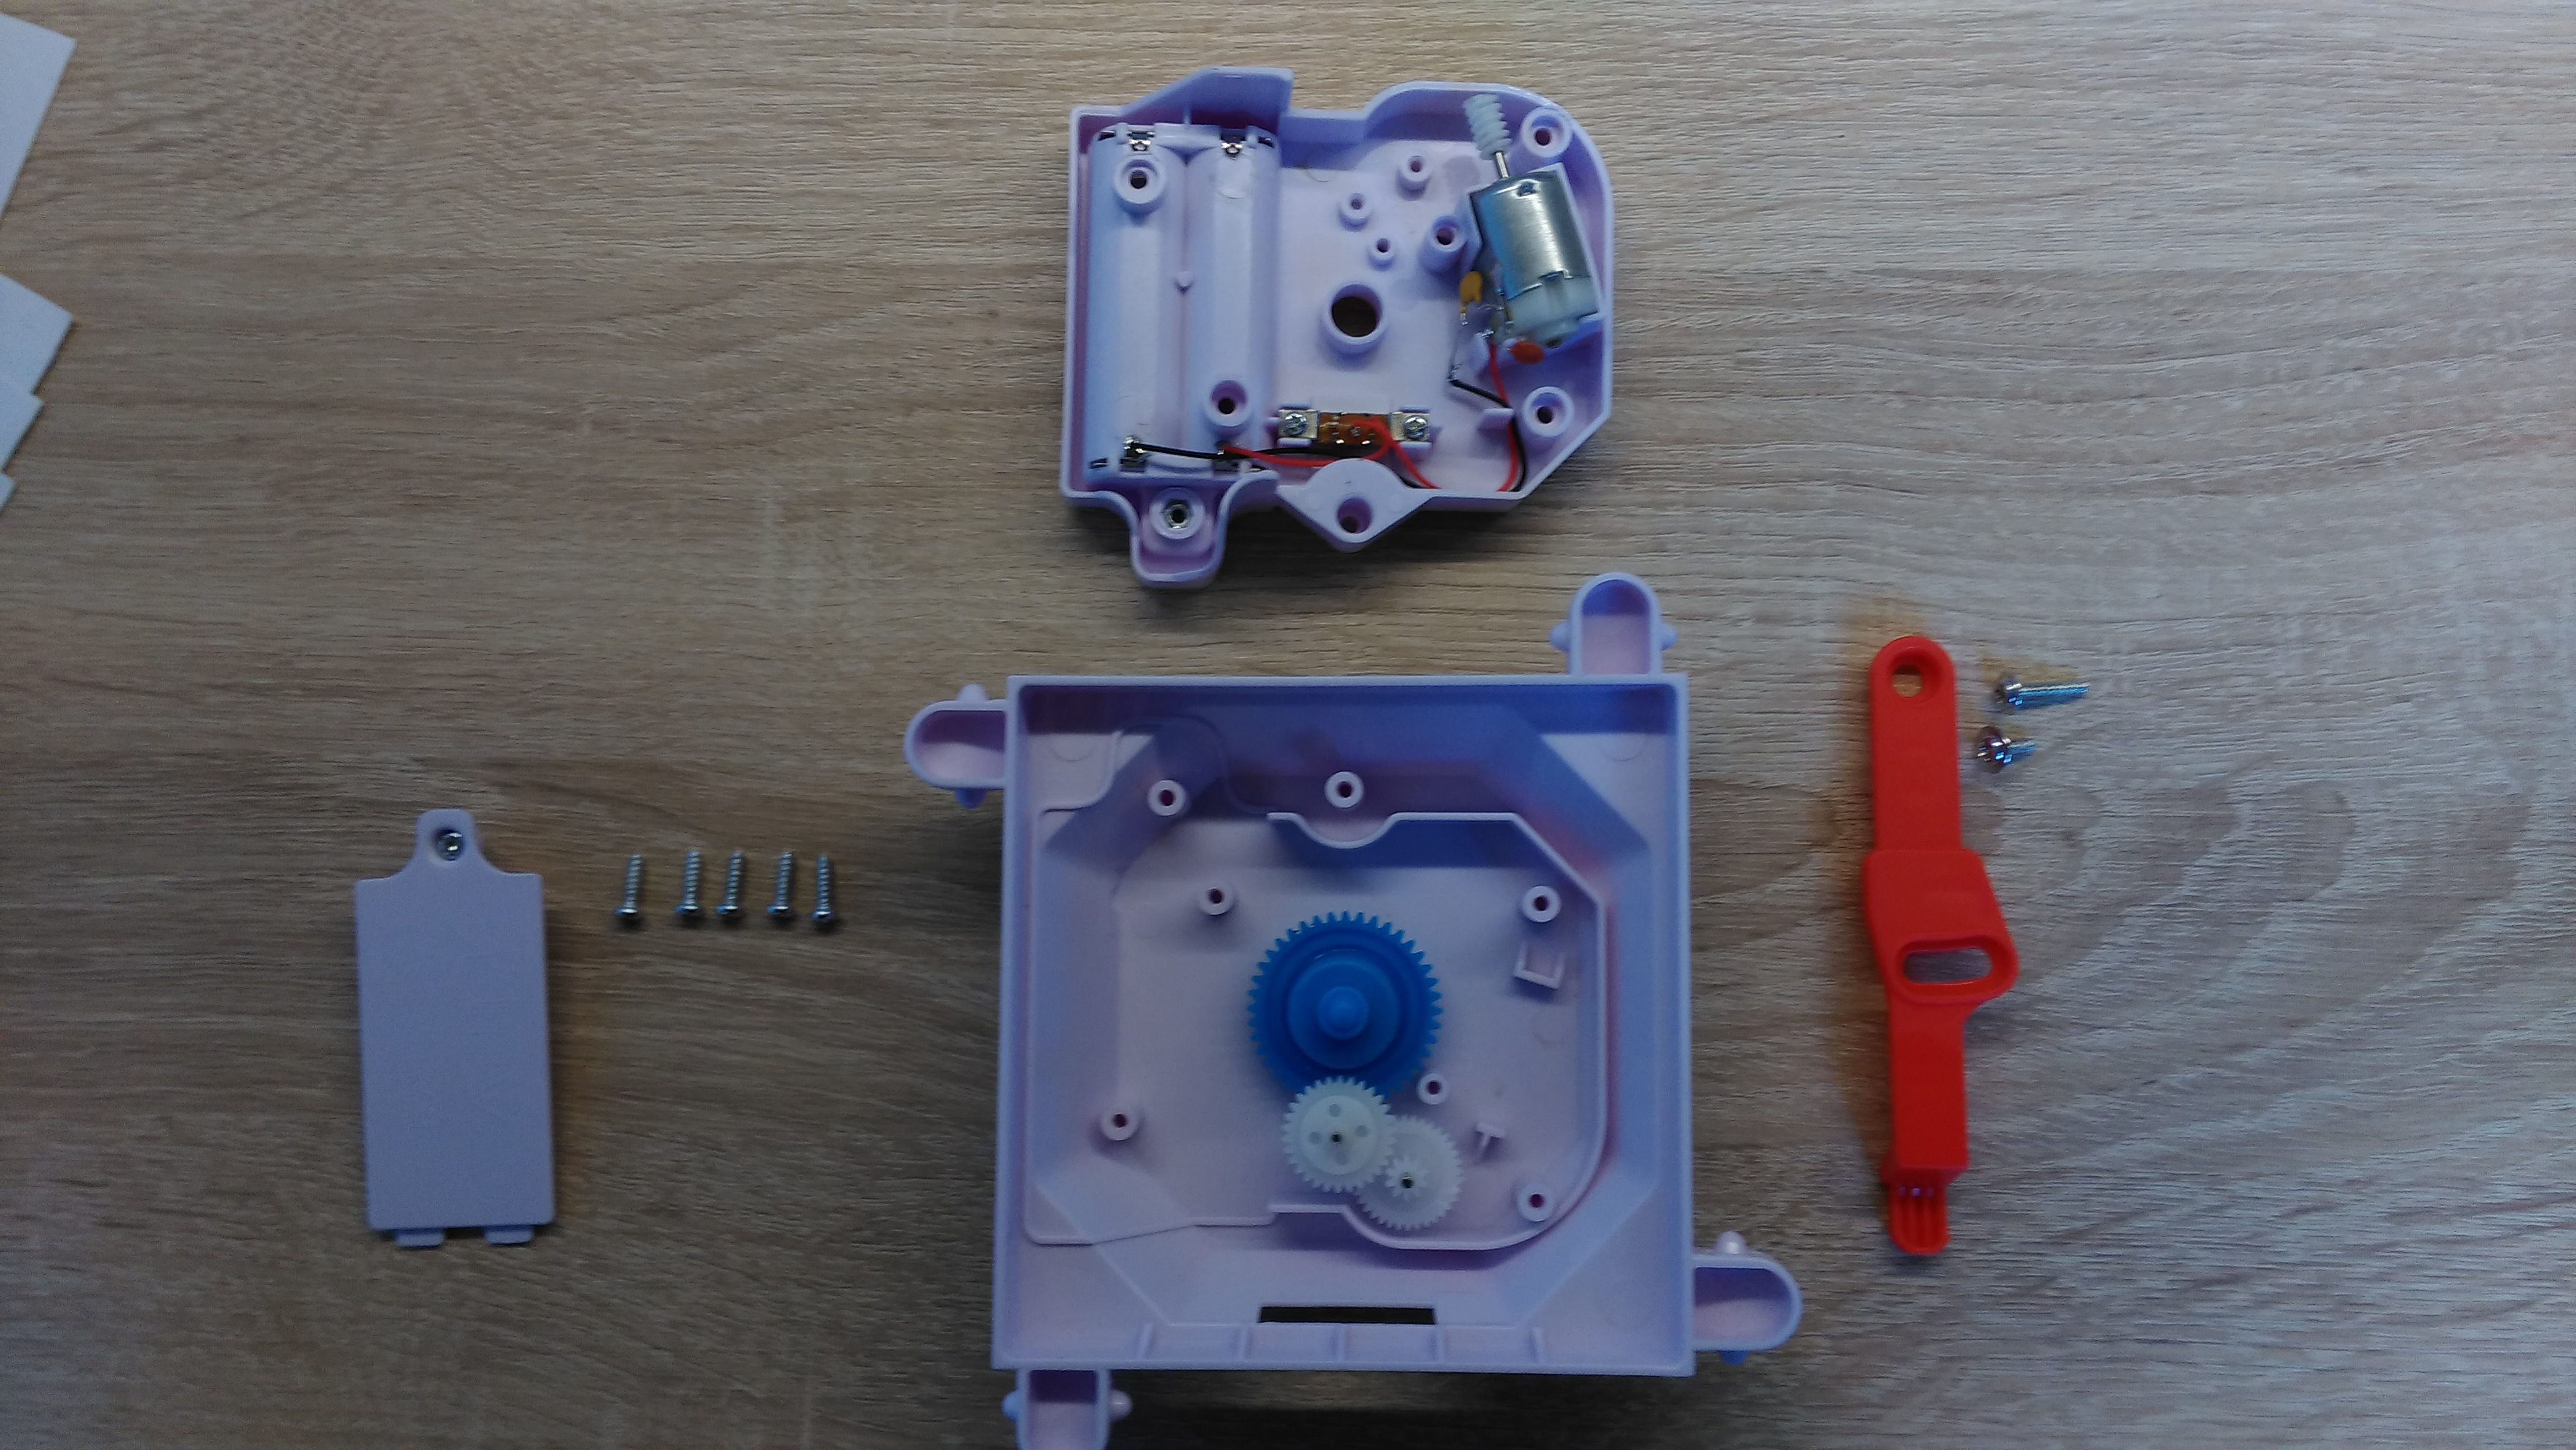
\includegraphics[width=0.7\textwidth]{pictures/loolou_004.jpg}
	\caption{Spielbasis - ge"offnet}
	\label{fig4}
\end{figure}
\vspace{1cm}
\begin{figure}[!ht]
	\centering
  	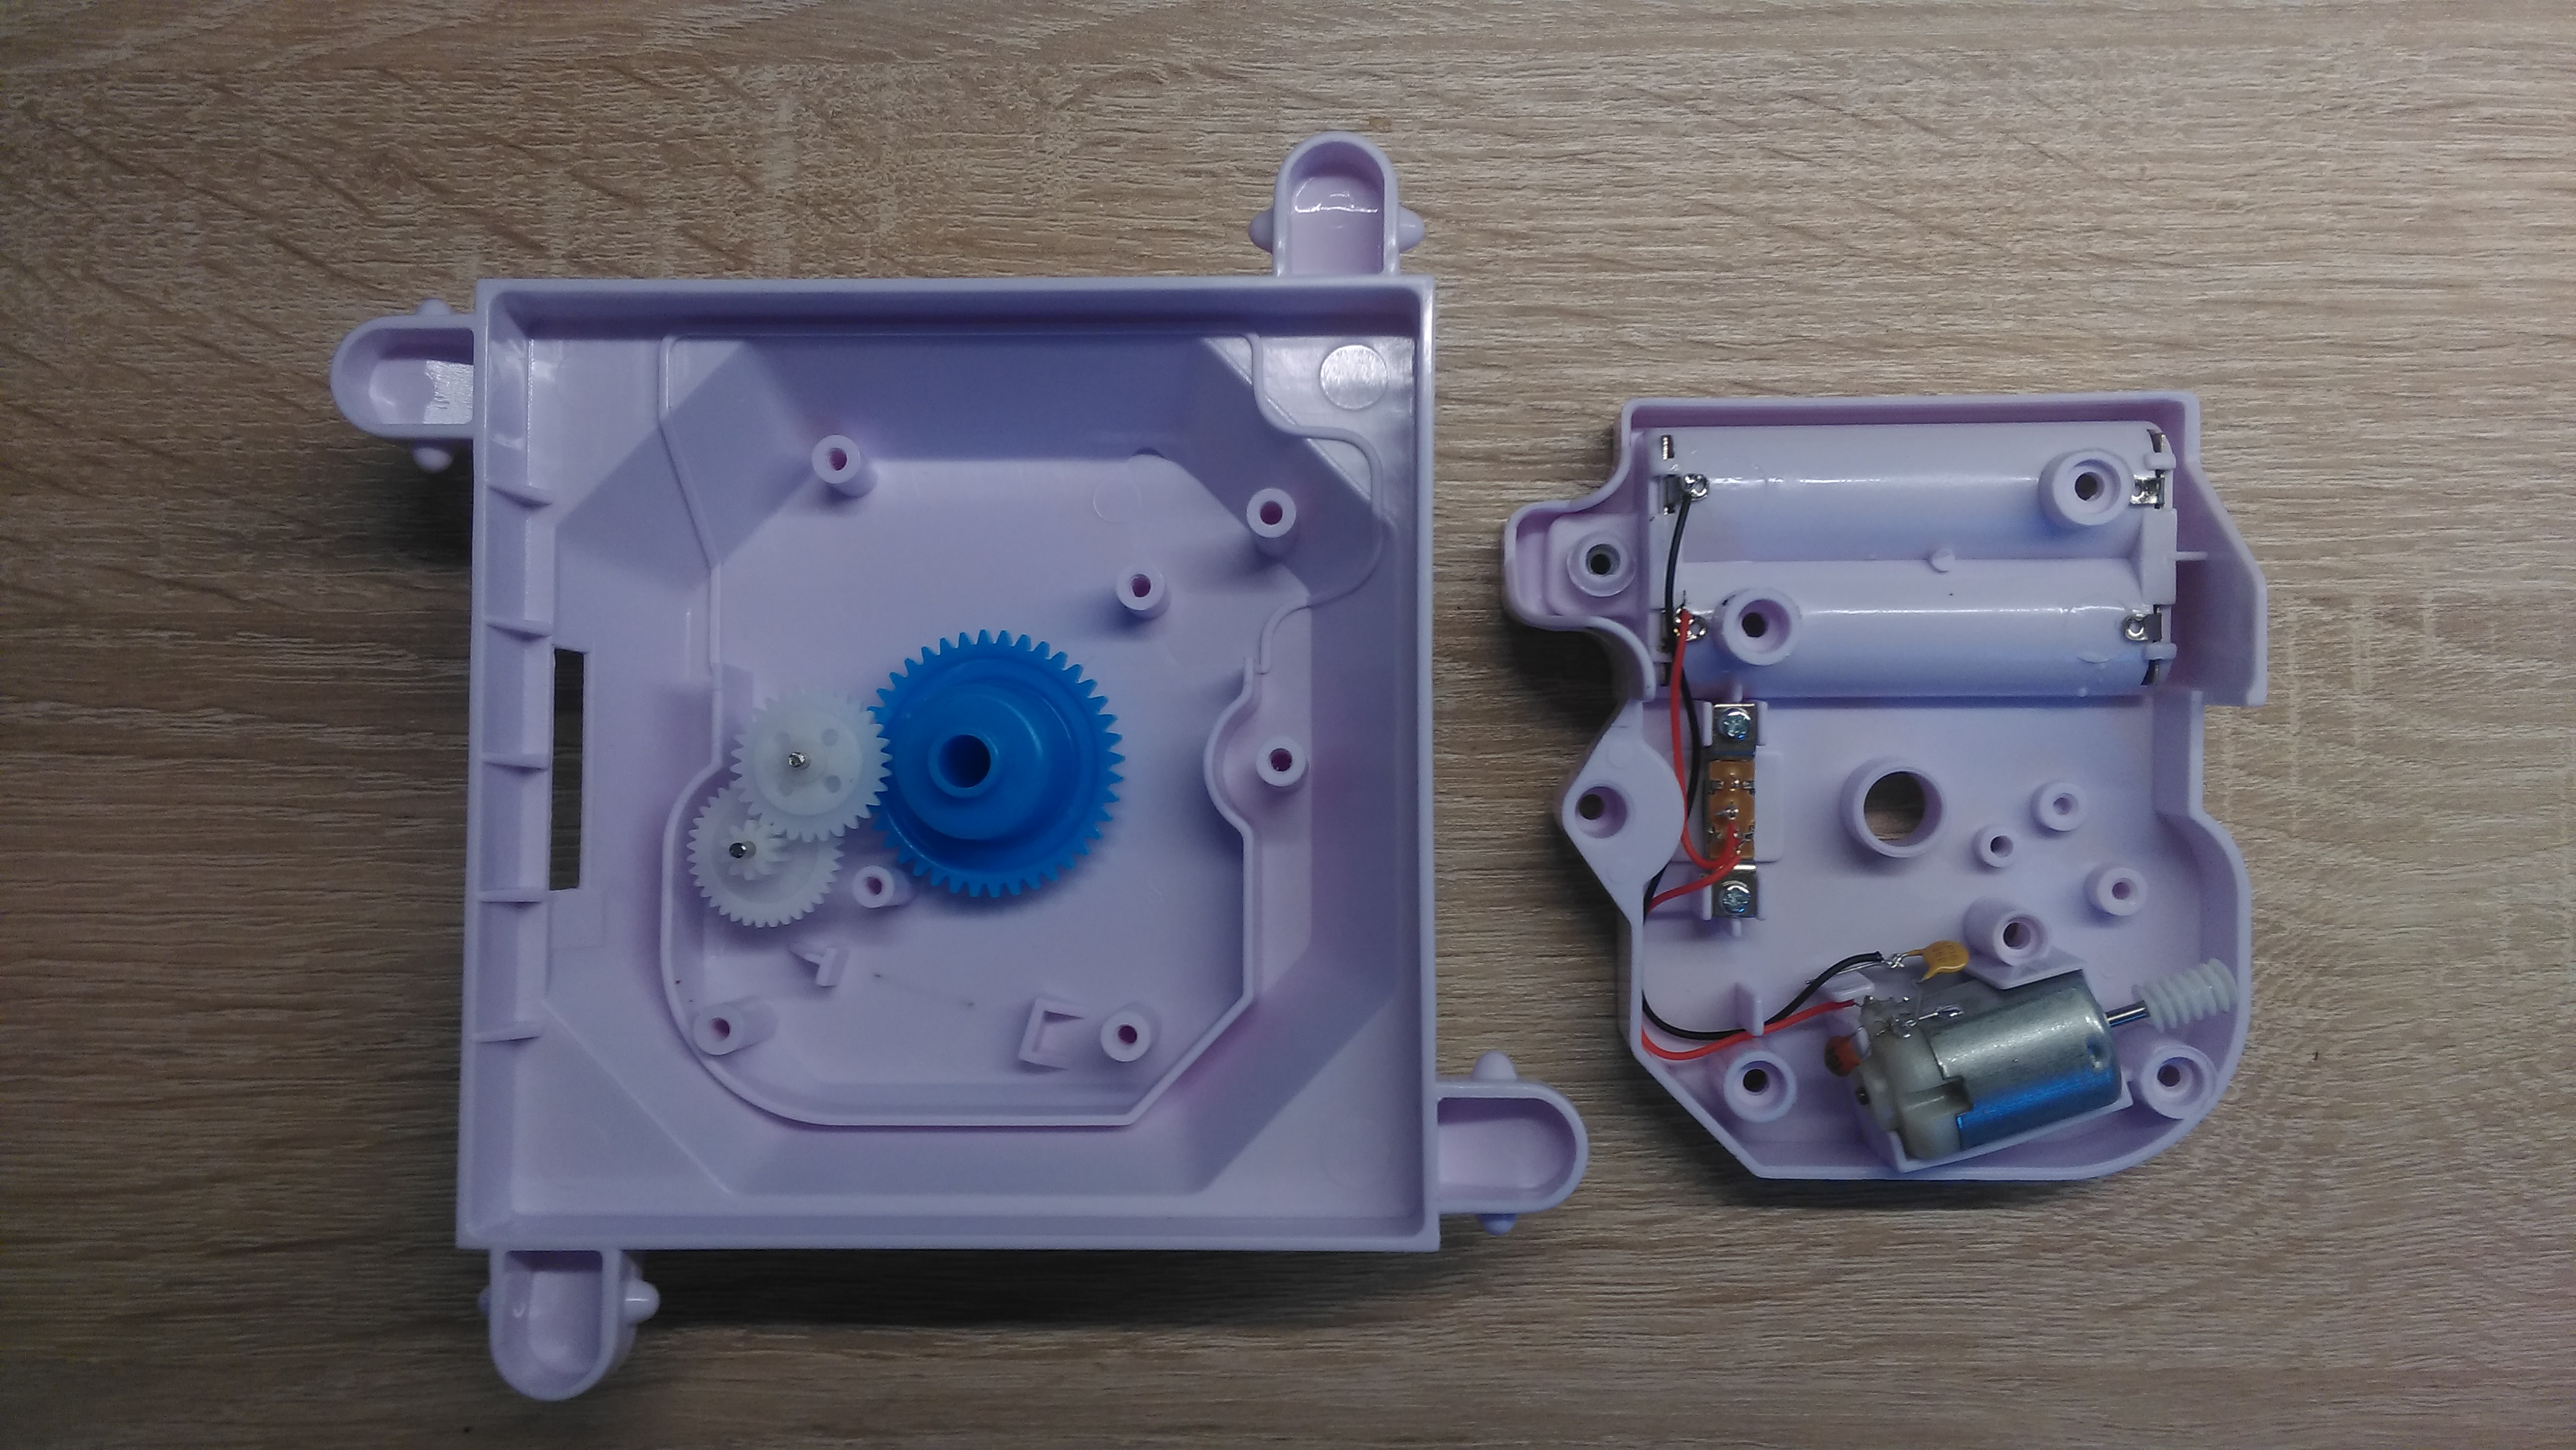
\includegraphics[width=0.7\textwidth]{pictures/loolou_005.jpg}
	\caption{Spielbasis - Abdeckung}
	\label{fig5}
\end{figure}
\vspace{0.5cm}

%\begin{figure}[!ht]
%	\centering
% 	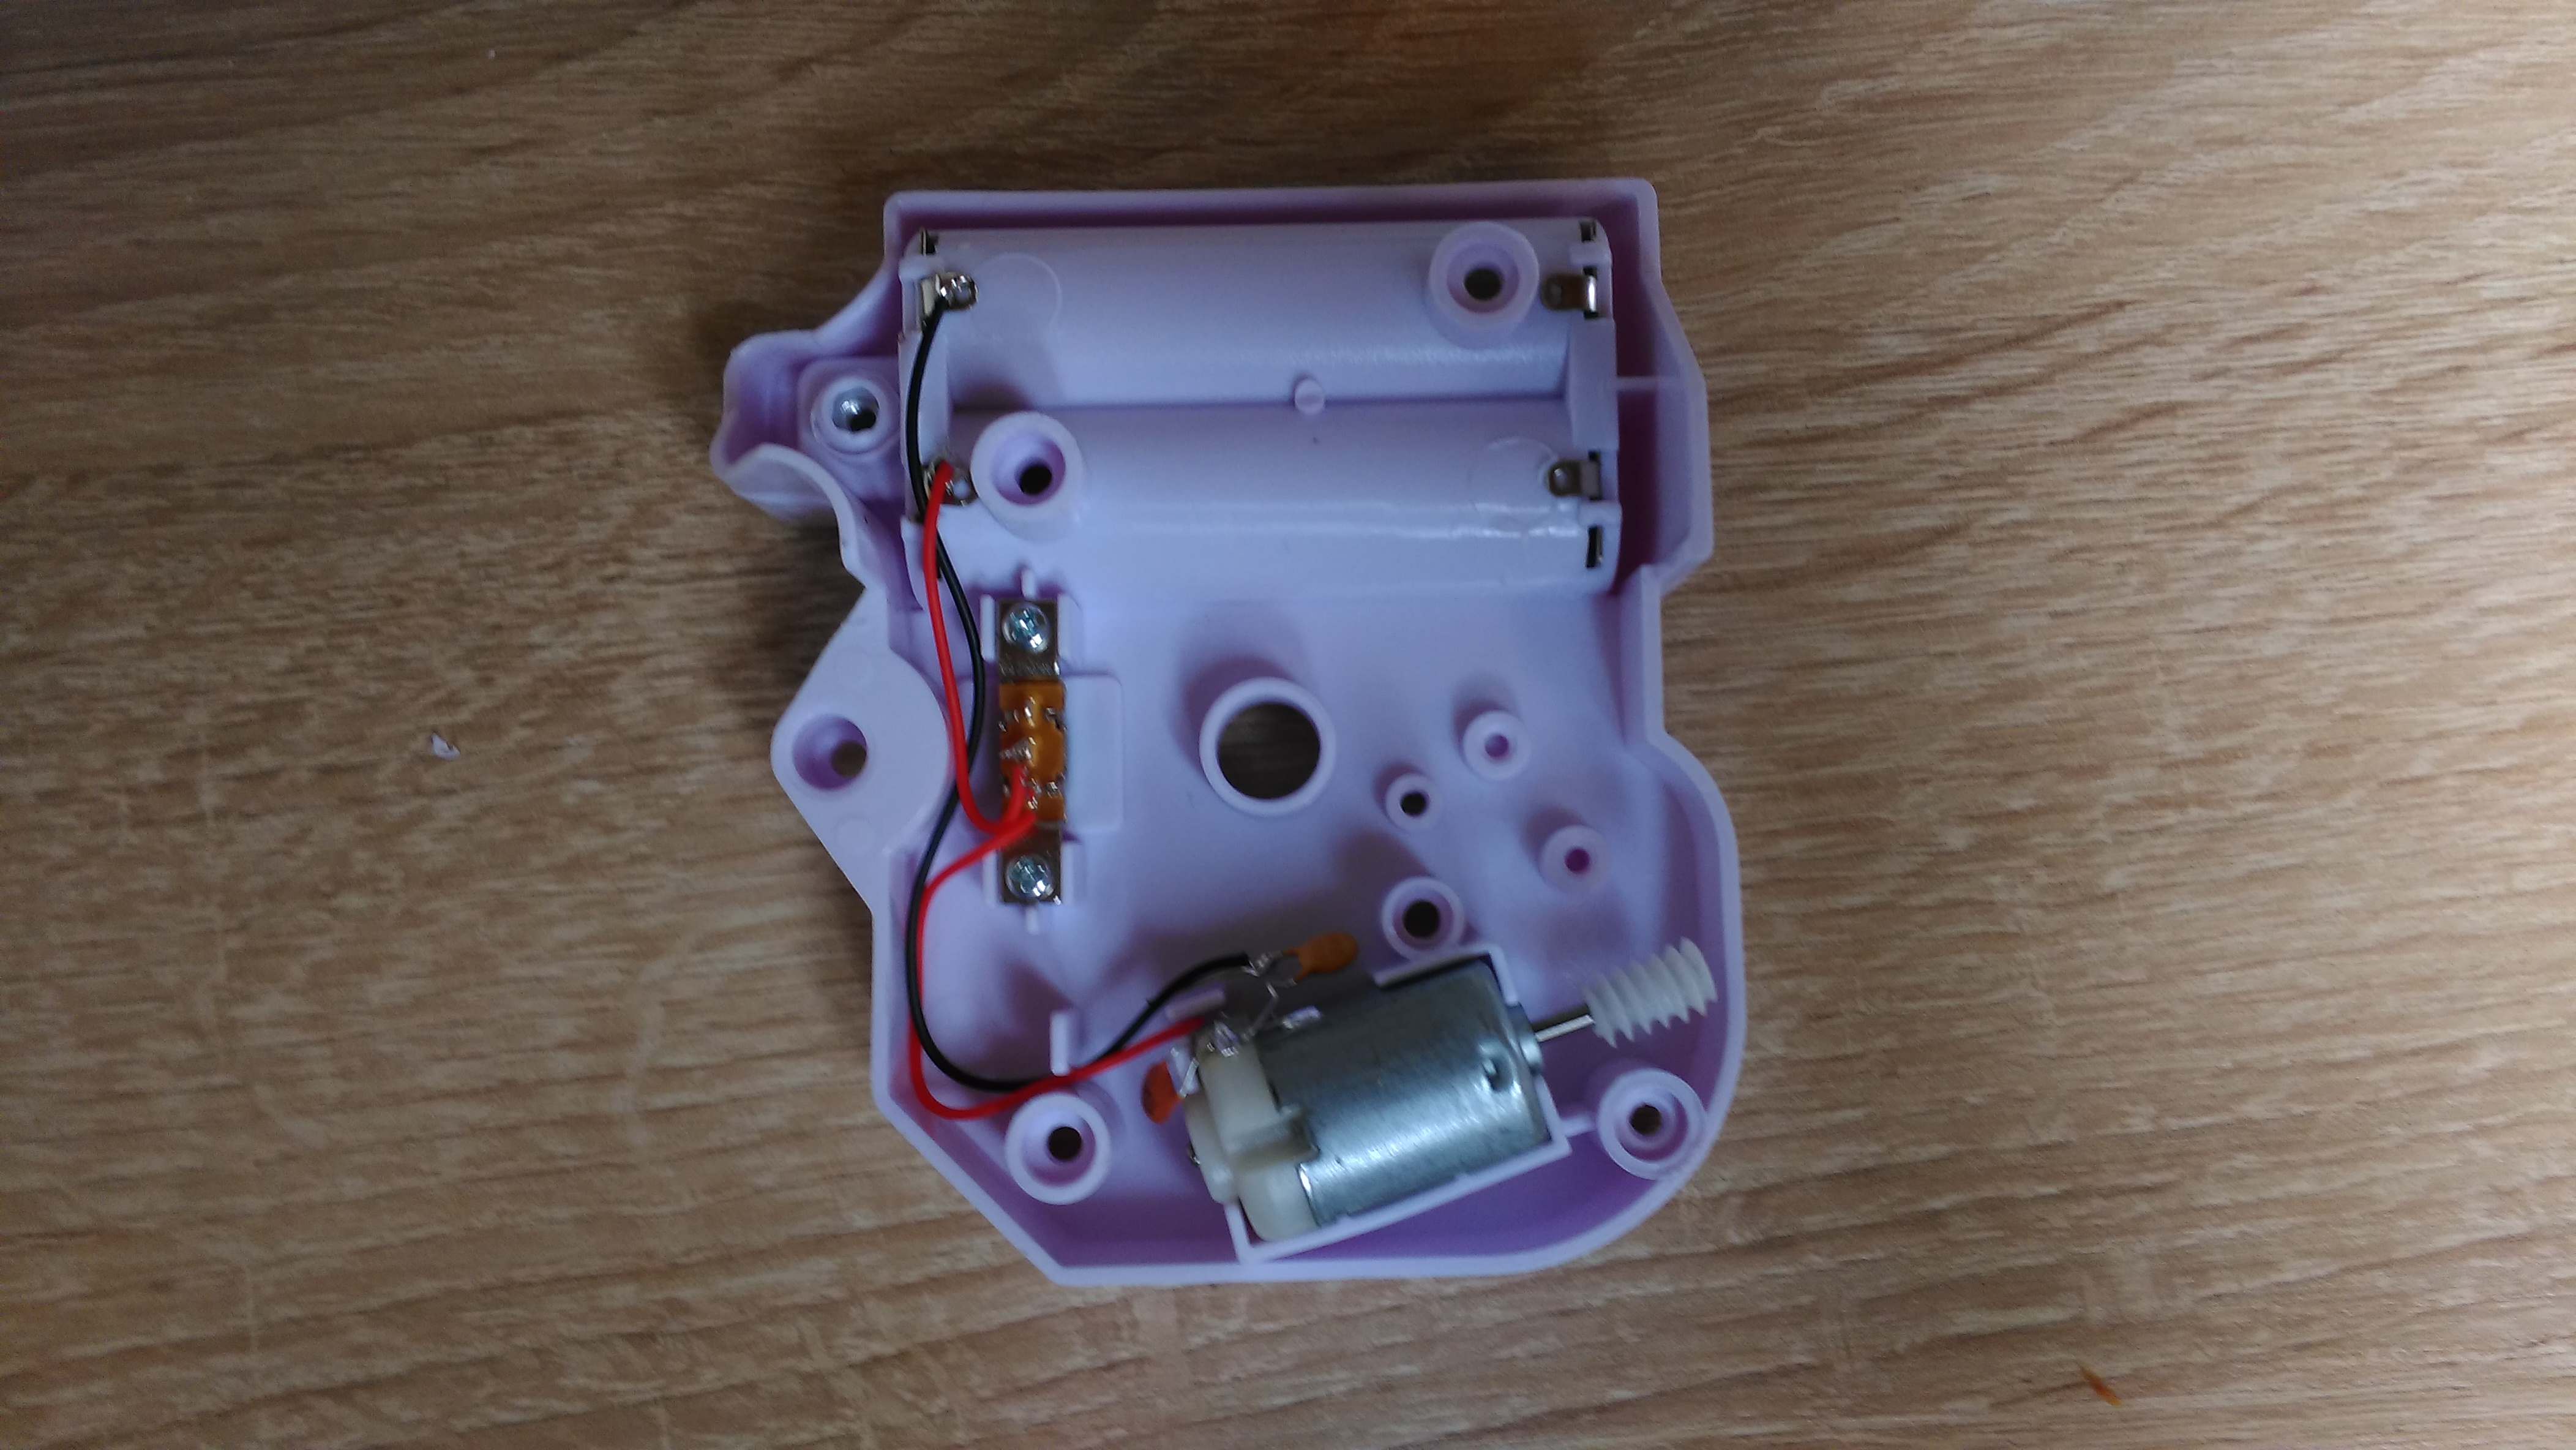
\includegraphics[width=0.7\textwidth]{pictures/loolou_006.jpg}
%	\caption{um 30 Grad gedreht}
%	\label{fig6}
%\end{figure}

Nun muss der Motor, der Stromschalter und die Batteriekontakte entfernt werden. \\
Am besten l"ost man hierf"ur zuerst die Stromkabel, mit einem L"otkolben, von den Batterie-Kontakten. \\
Anschlie"send kann der Motor ganz einfach herausgezogen und der Stromschalter mittels eines Schraubenziehers entfernt werden.
Danach k"onnen die Batteriekontakte mit einer Zange herausgezogen werden.
Abbildung ~\ref{fig7} zeigt die Abdeckung der Spielbasis ohne Motor, Stromschalter und Batteriekontakte.

\vspace{1cm}
\begin{figure}[!ht]
	\centering
  	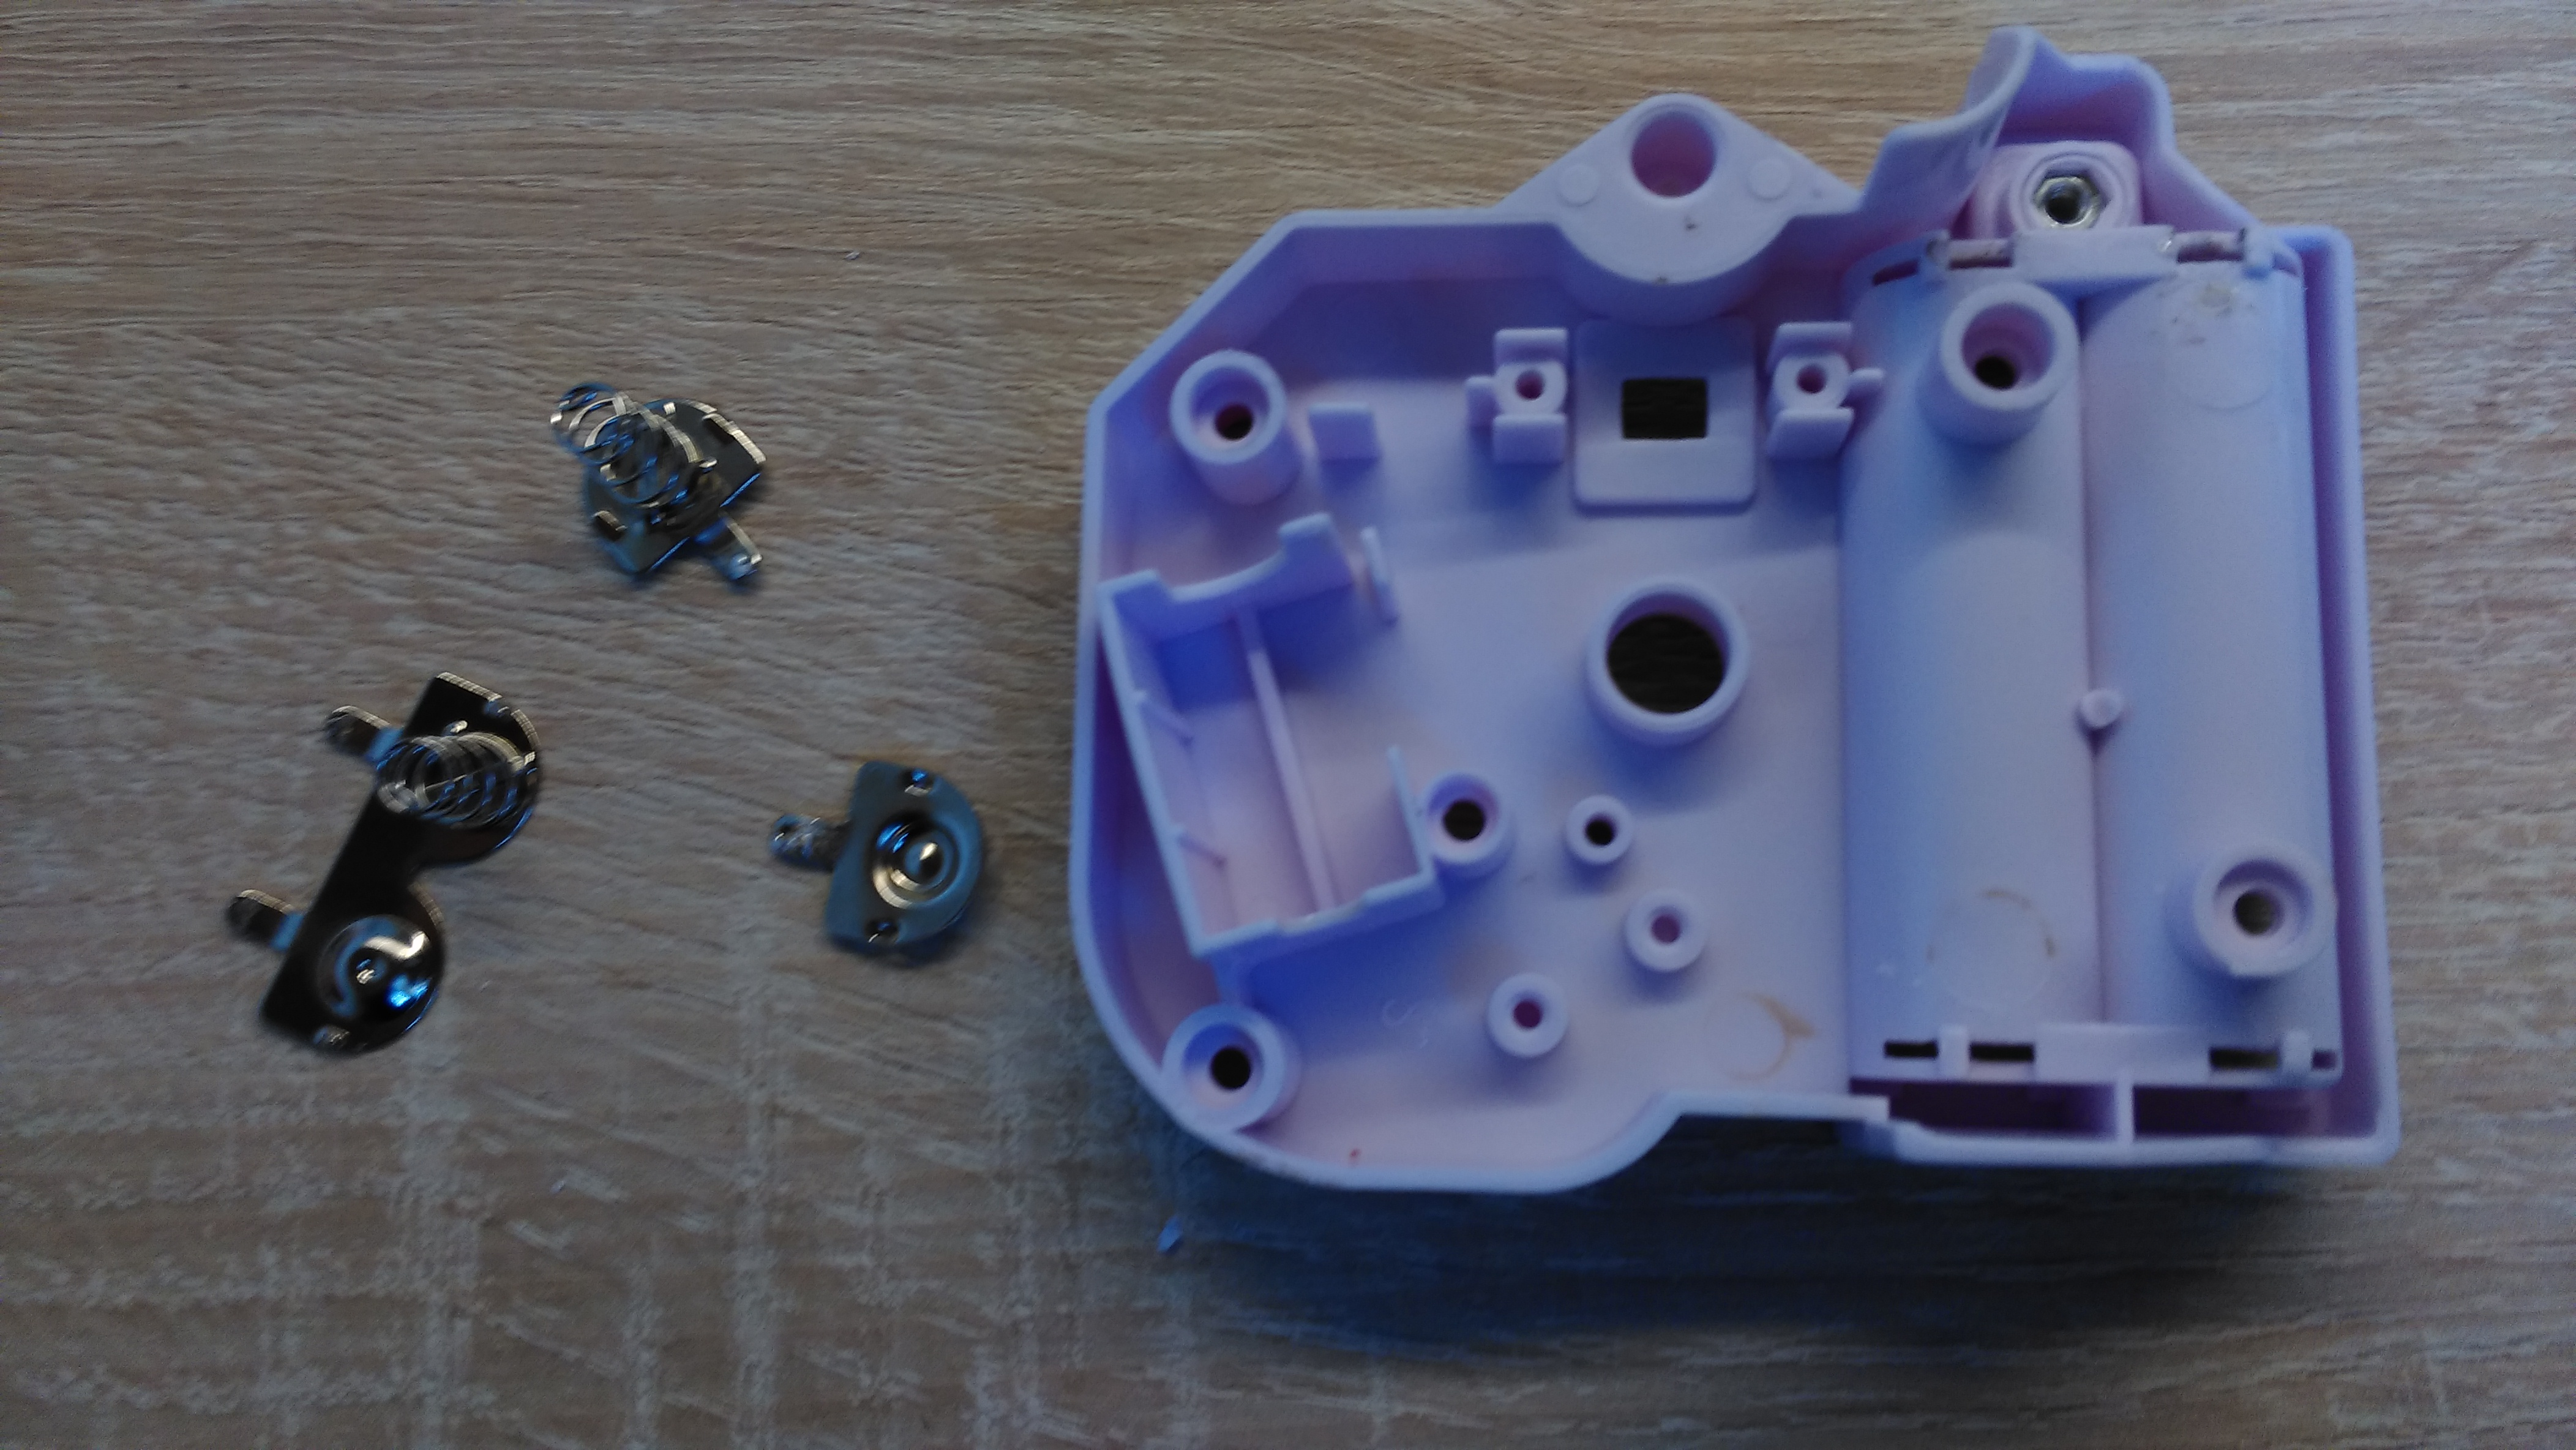
\includegraphics[width=0.7\textwidth]{pictures/loolou_007.jpg}
	\caption{Spielbasis - Unterseite Abdeckung ohne Motor und Batteriekontakten}
	\label{fig7}
\end{figure}
\vspace{0.5cm}

Als n"achstes muss Platz f"ur die Platine geschaffen werden. \\ 
Dazu bohrt man an den 4 Ecken des Batteriefaches jeweils ein Loch in die Abdeckung und s"agt mit einer S"age am Rand des Batteriefaches entlang (zu sehen in Abbildung ~\ref{fig8}). \\
Achte an dieser Stelle besonders auf das Geh"ause - Es sollte nicht brechen bzw. es sollte nicht weiter als die Umrandung das Batteriefach ges"agt werden. Ansonsten sieht man beim sp"ateren zusammen bauen, des Geh"auses, die Schnitte der S"age. Ebenso sollten keine Gewinde für die Schrauben, mit Ausnahme der Gewinde im Batteriefach, abges"agt werden. 
F"ur die feineren Arbeiten kann eine Feile benutzt werden. 
Anschließend muss in den herausstehenden Seiten der Unterseite jeweils eine Ecker herausgefeilt werden (Gut zu sehen in der Abbildung ~\ref{fig9}). Diese werden sp"ater ben"otigt um die Stromkabel für die LEDs und des Netzger"ates aus der Spielbasis herauszuf"uhren.  

\vspace{1cm}
\begin{figure}[!ht]
	\centering
  	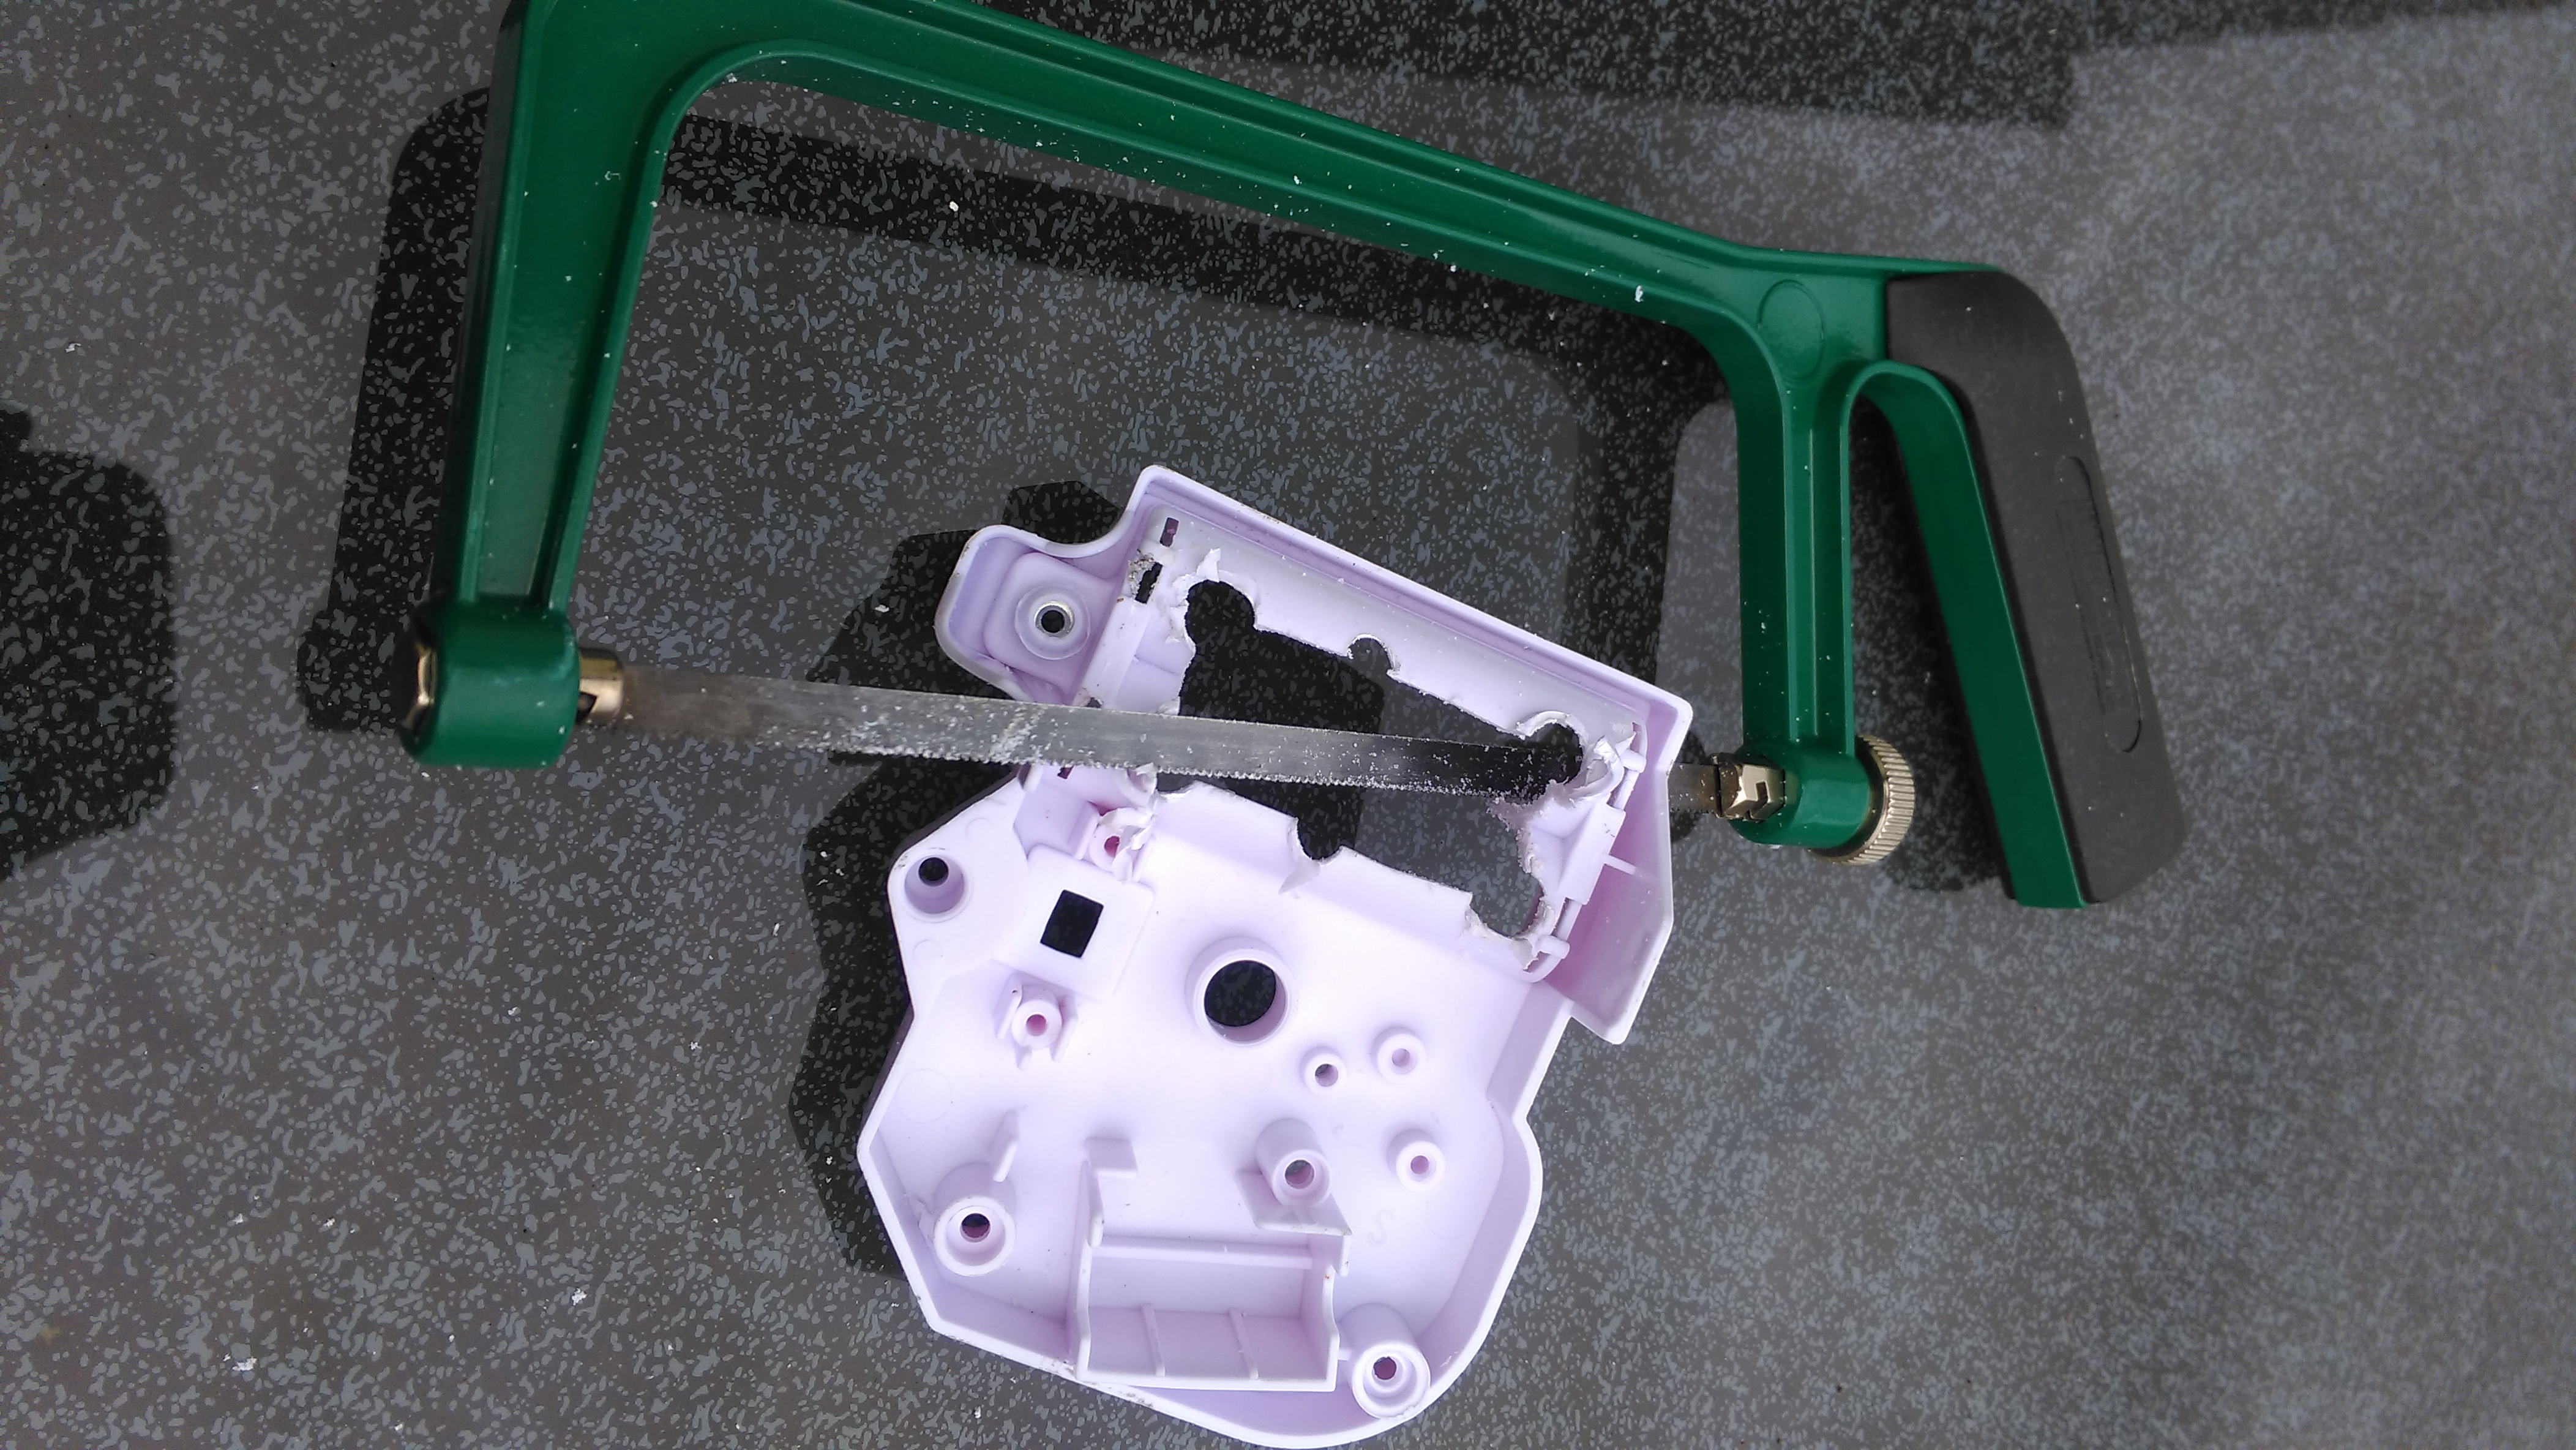
\includegraphics[width=0.7\textwidth]{pictures/loolou_008.jpg}
	\caption{Spielbasis - Unterseite beim auss"agen}
	\label{fig8}
\end{figure}
\vspace{0.5cm}

Abbildung ~\ref{fig9} zeigt die fertig vorbereitete Unterseite der Spielbasis. Gut zu sehen sind hier die abgefeilten Ecken f"ur die Stromkabel und das ausges"agte Batteriefach.
Wichtig an dieser Stelle ist auch, dass das Batteriefach vollst"antig entfernt und bis auf den letzten Millimeter abgefeilt wurde. Ansonsten kann es vorkommen, dass das Geh"ause beim sp"ateren Zusammenbau nicht richtig schlie"st.

\vspace{1cm}
\begin{figure}[!ht]
	\centering
  	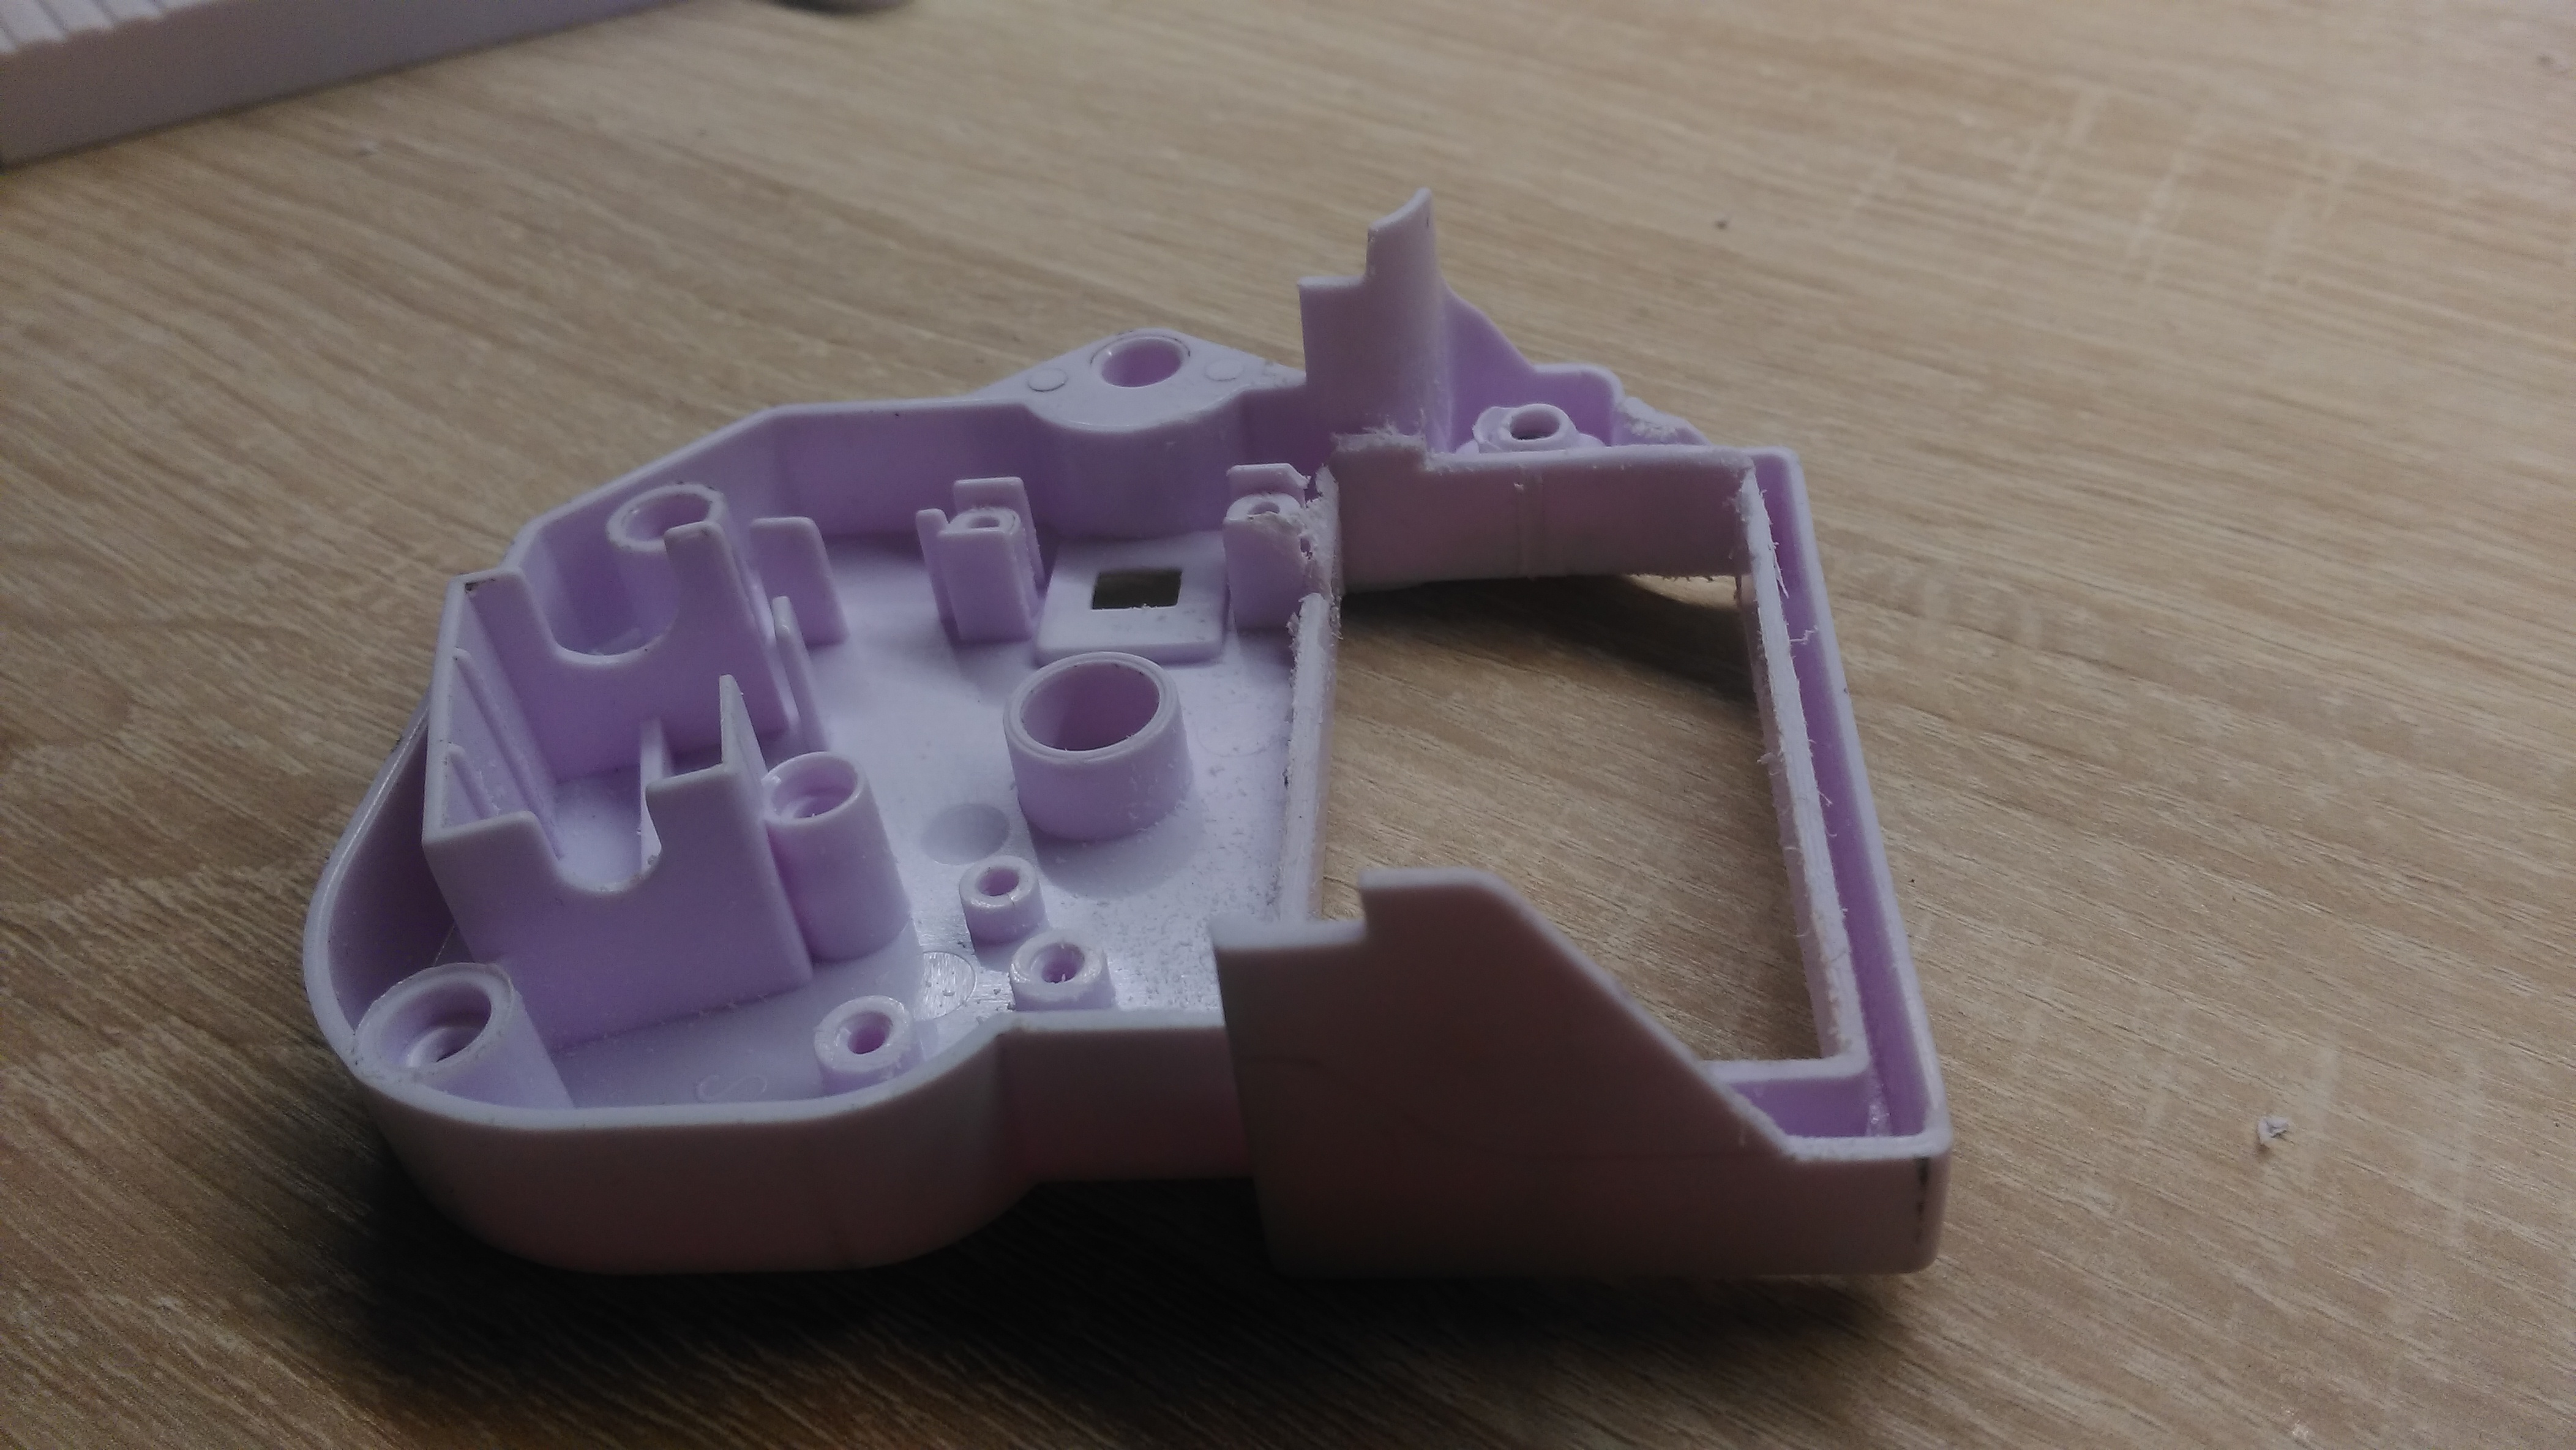
\includegraphics[width=0.7\textwidth]{pictures/loolou_009.jpg}
	\caption{Spielbasis - Unterseite ausges"agt und geschliffen}
	\label{fig9}
\end{figure}
\vspace{0.5cm}

Nun kann die Unterseite der Spielbasis zur Seite gelegt werden. Es folgt die Vorbereitung der Oberseite. \\
Als erstes sollte hier das Gewinde im linken oberen Eck (siehe Abbildung ~\ref{fig10}) mit einem Bohrer entfernt werden. Dieses Gewinde ist der Platine im Weg und muss daher entfernt werden.
Achte hierbei darauf das nicht durch das Oberteil gebohrt wird, lasse lieber ein bis zwei Millimeter "uberstehen.
 
\vspace{1cm}
\begin{figure}[!ht]
	\centering
  	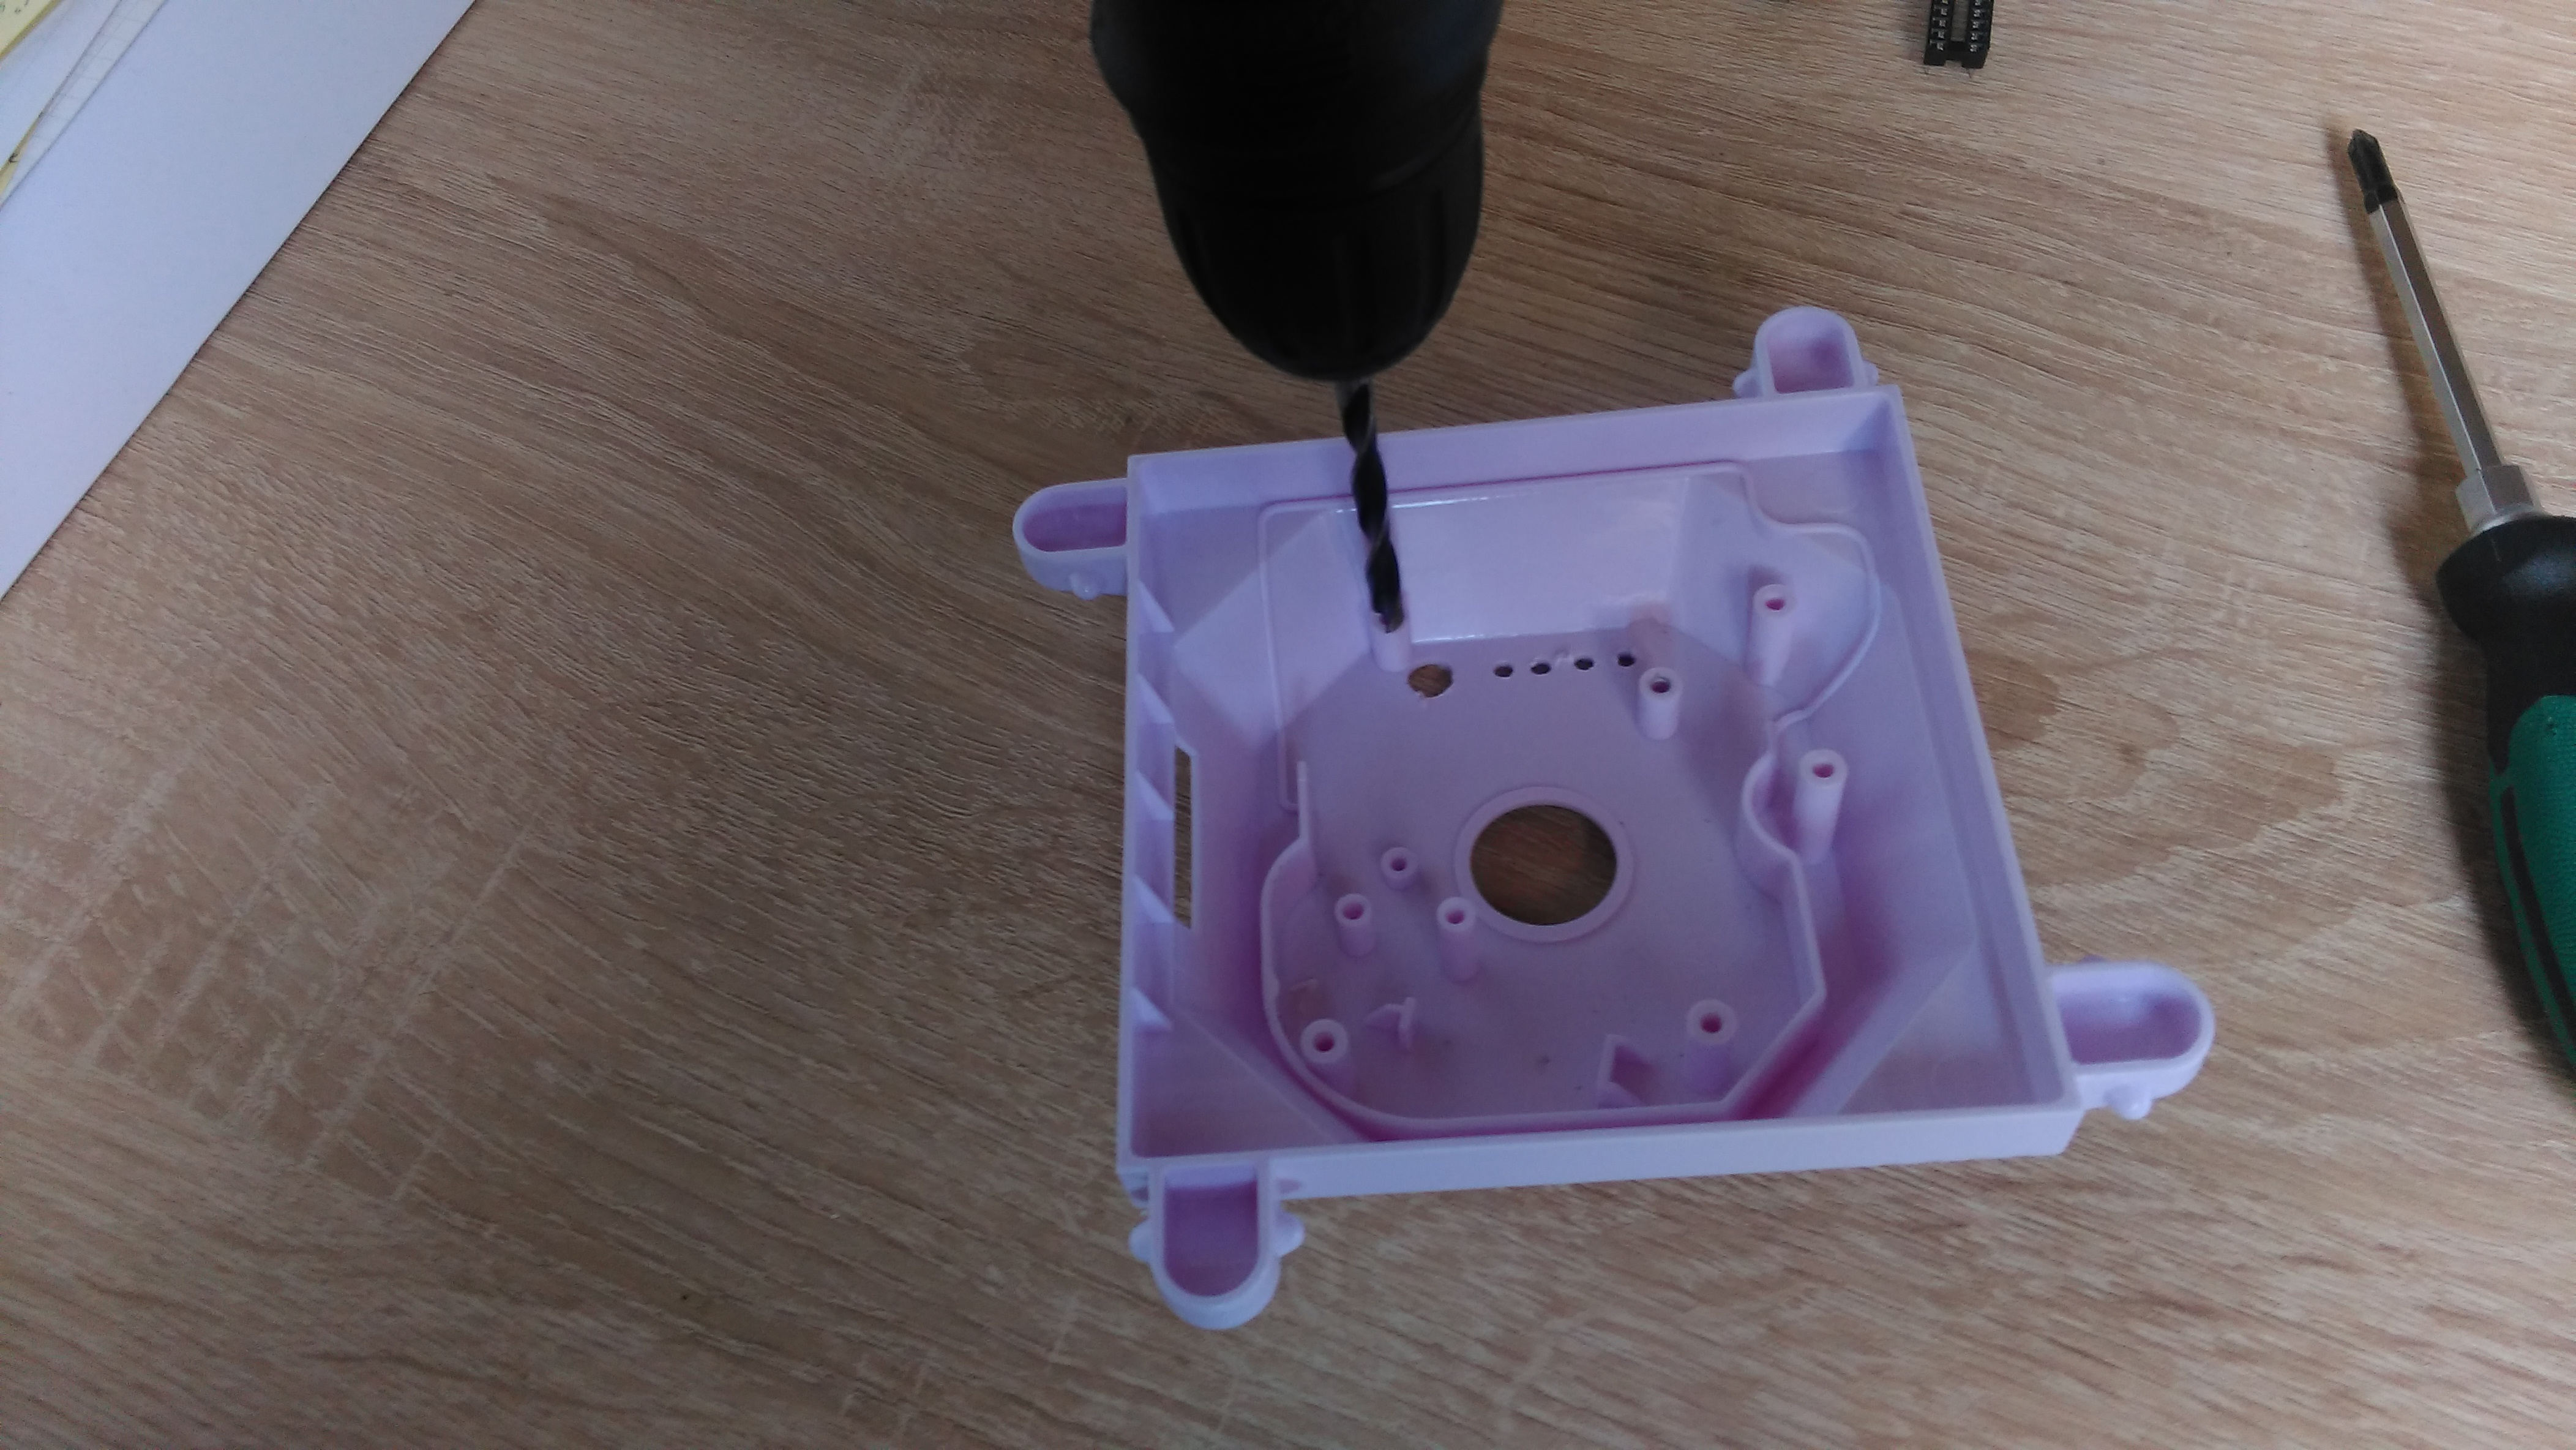
\includegraphics[width=0.7\textwidth]{pictures/loolou_010.jpg}
	\caption{Spielbasis - Oberseite mit Gewinde das entfertn werden muss}
	\label{fig10}
\end{figure}
\vspace{0.5cm}

%\begin{figure}[!ht]
%	\centering
% 	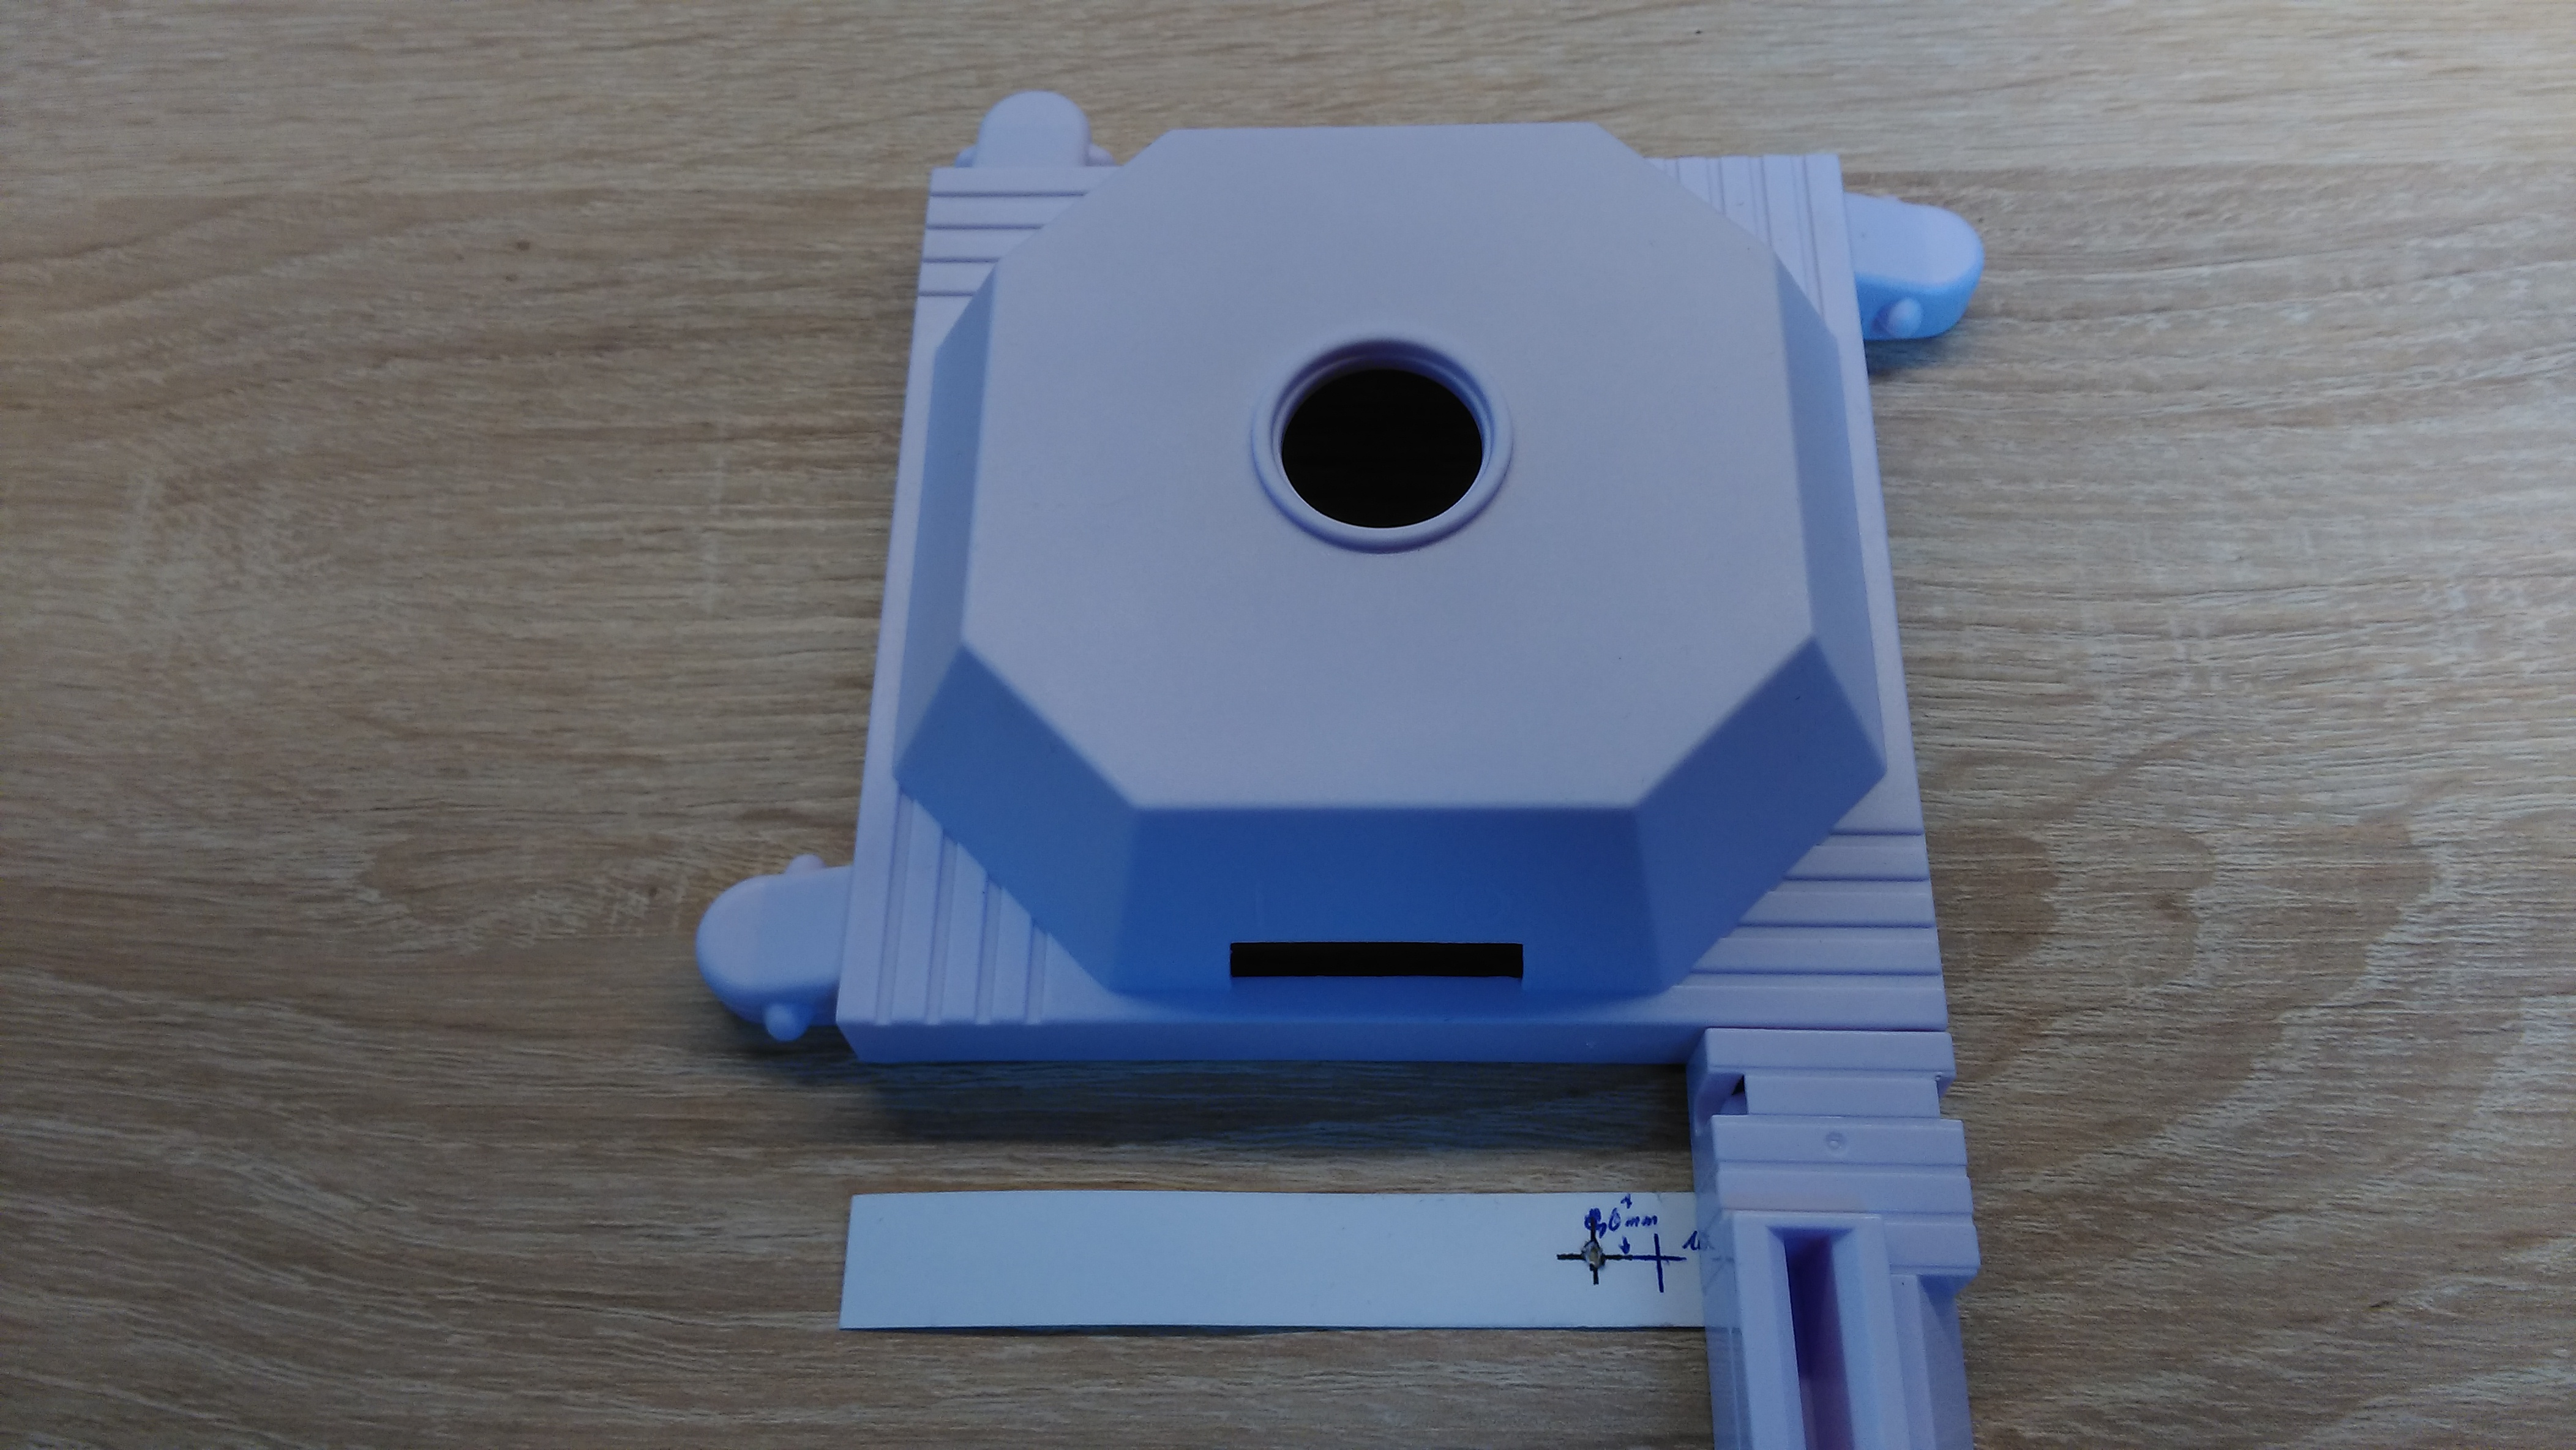
\includegraphics[width=0.7\textwidth]{pictures/loolou_011.jpg}
%	\caption{um 30 Grad gedreht}
%	\label{fig11}
%\end{figure}

Als n"achstes schneidet man zuerst die Schablonen (siehe Anhang ~\ref{appendix1}) aus. Diese werden ben"otigt um die L"ocher f"ur die LEDs, den Taster und den Stromanschlu"s richtig zu positionieren.
Abbildung ~\ref{fig12} zeigt die Schablonen und das fertig Vorbereitete Geh"ause.

\vspace{1cm}
\begin{figure}[!ht]
	\centering
  	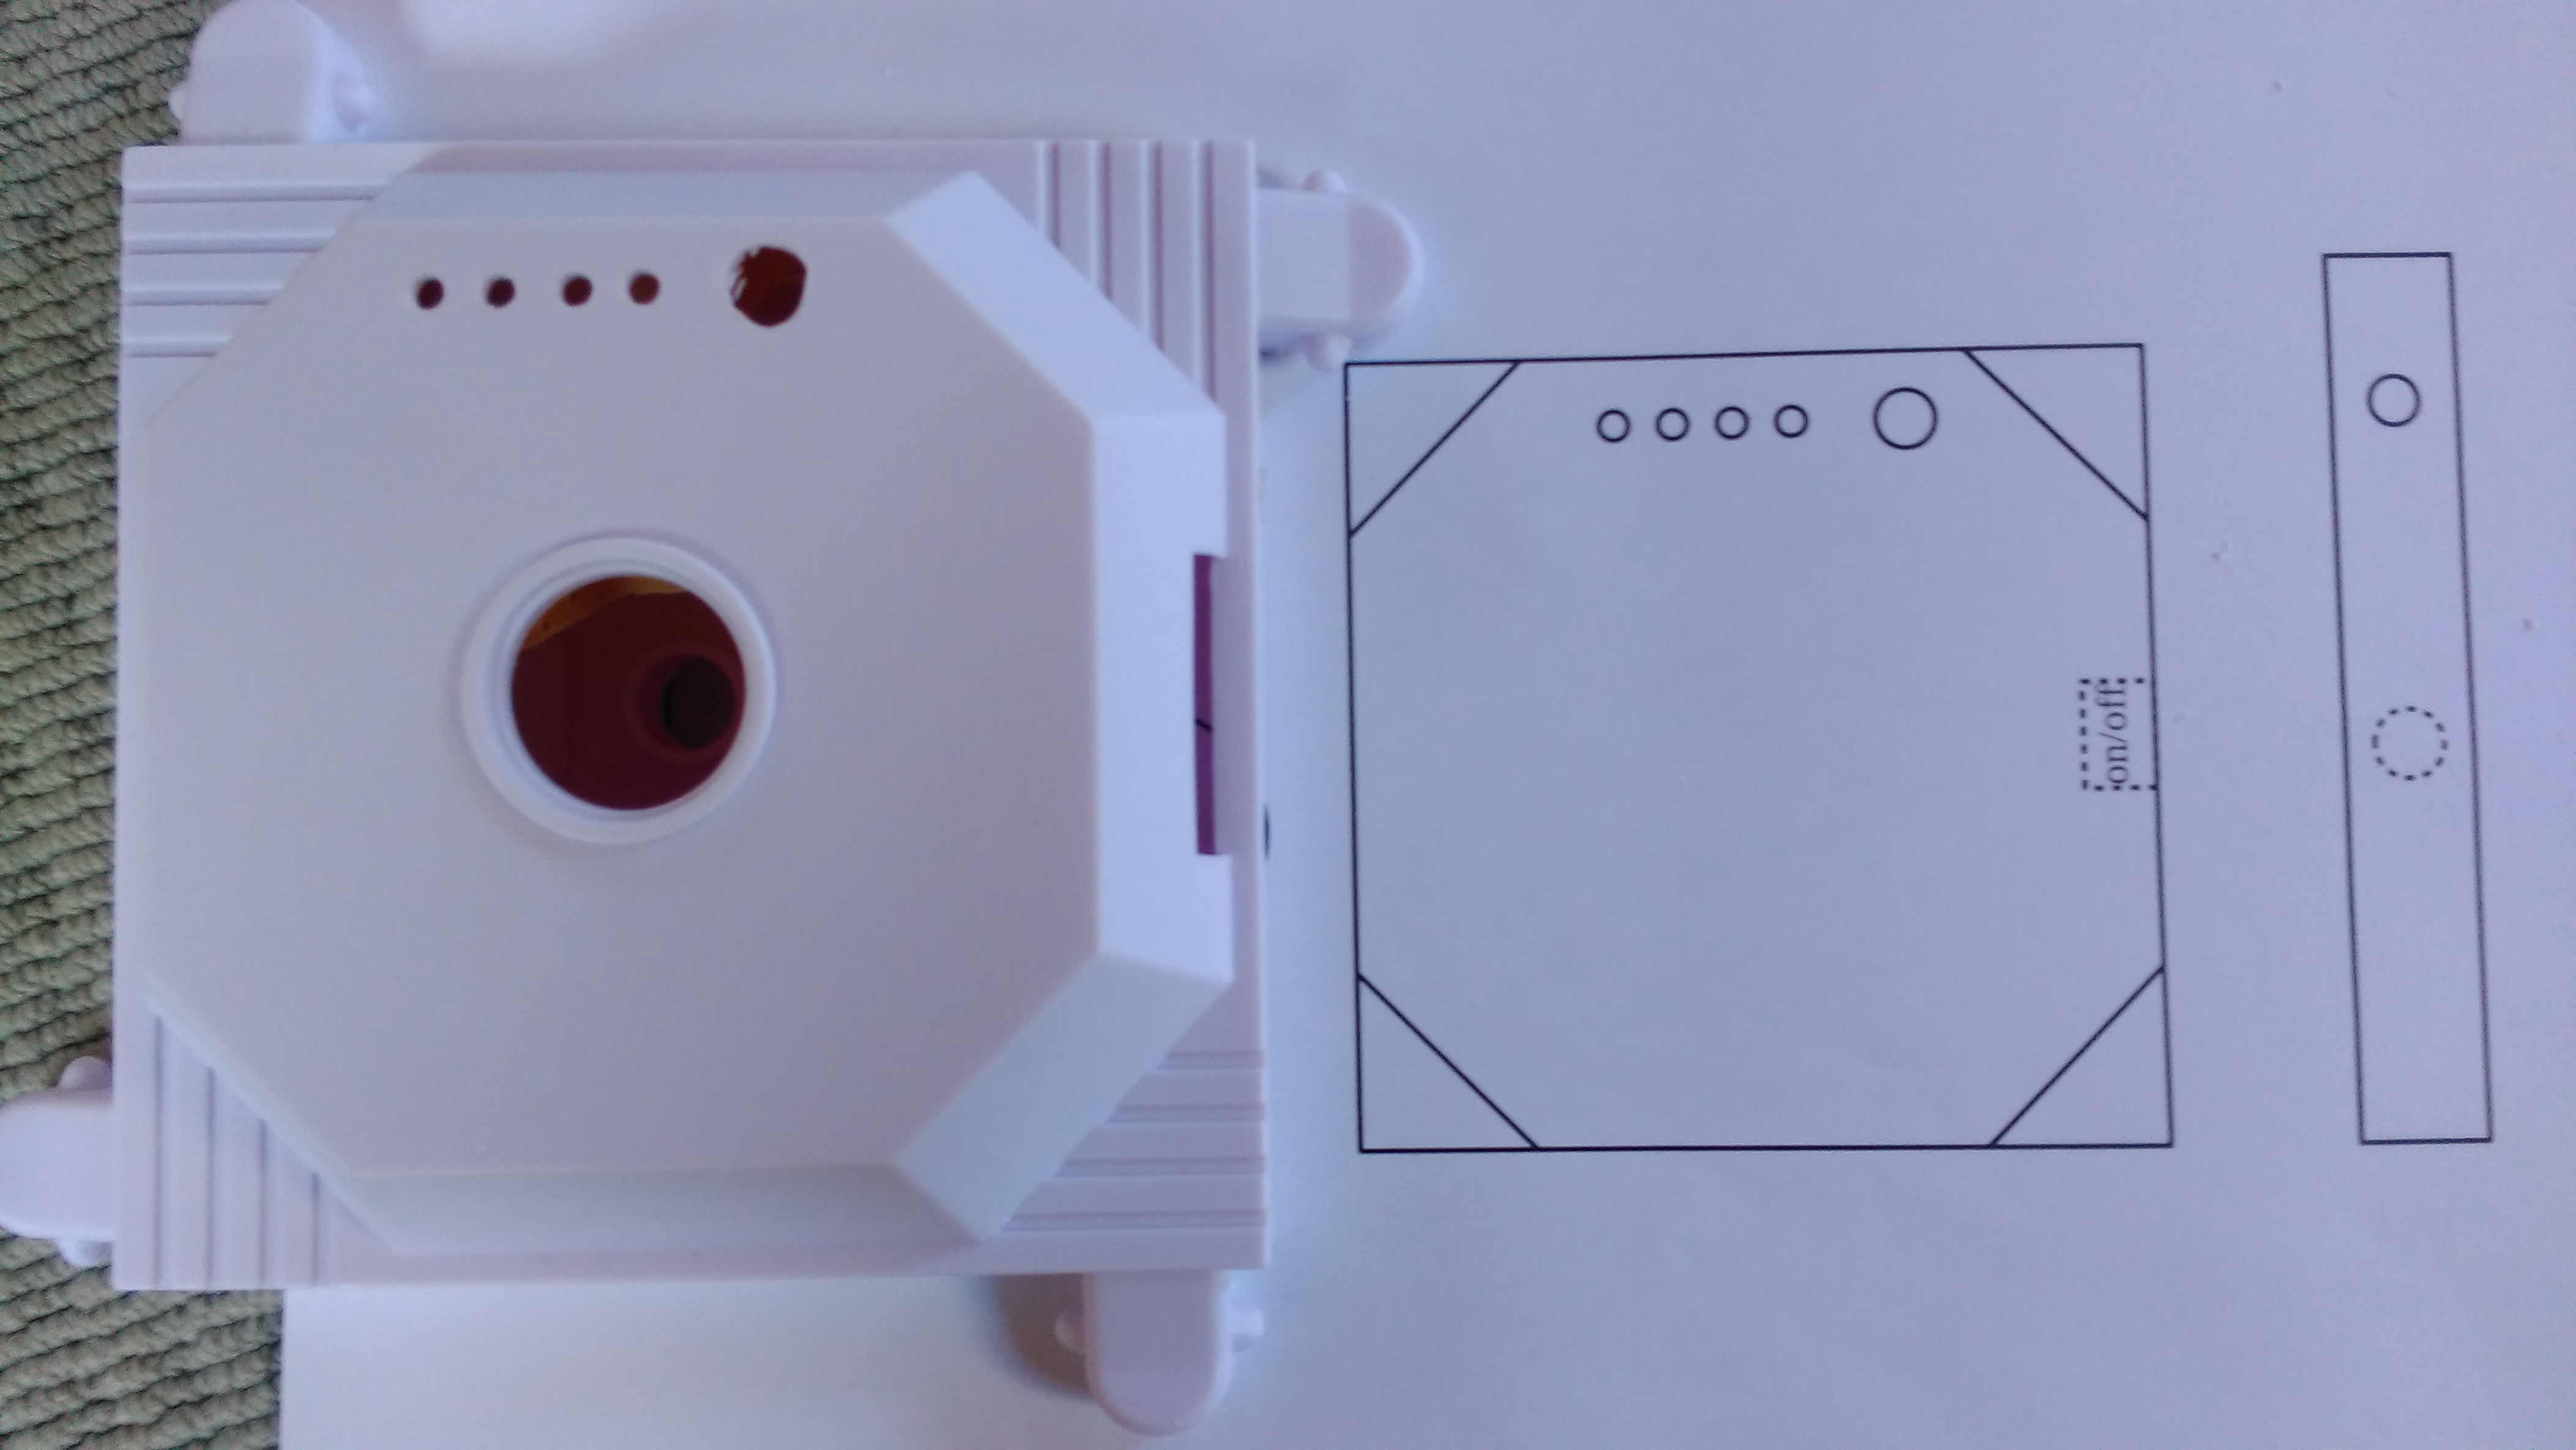
\includegraphics[width=0.7\textwidth]{pictures/loolou_012.jpg}
	\caption{Schablonen und Oberteil der Spielbasis}
	\label{fig12}
\end{figure}
\vspace{0.5cm}

Im n"achsten Schritt nimmt man das gro"se Teil der Schablone und legt dieses Auf die Oberseite der Spielbasis. Man sollte hier darauf achten das die Schrift \grqq on/off\grqq  "uber dem AN/AUS-Schalter der Spielbasis liegt. Anschließend kann zuerst mit einem spitzen Gegenstand (zum Beispiel einem Bohrer) die L"ocher auf dem Oberteil der Spielbasis angek"ornt werden.
Die kleinen L"ocher, f"ur die LEDs, werden nun mit einem 3mm durchbohrt. Im Anschluss wird das Loch f"ur den Drucktaster mit einem 7mm Bohrer in das Oberteil gebohrt. 
Abbildung ~\ref{fig13} zeigt die gebohrten L"ocher in dem Oberteil der Spielbasis. Zu sehen ist hier auch das die L"ocher auf der rechten Seiten, vom AN/AUS-Schalter aus gesehen, liegen.  

\vspace{1cm}
\begin{figure}[!ht]
  	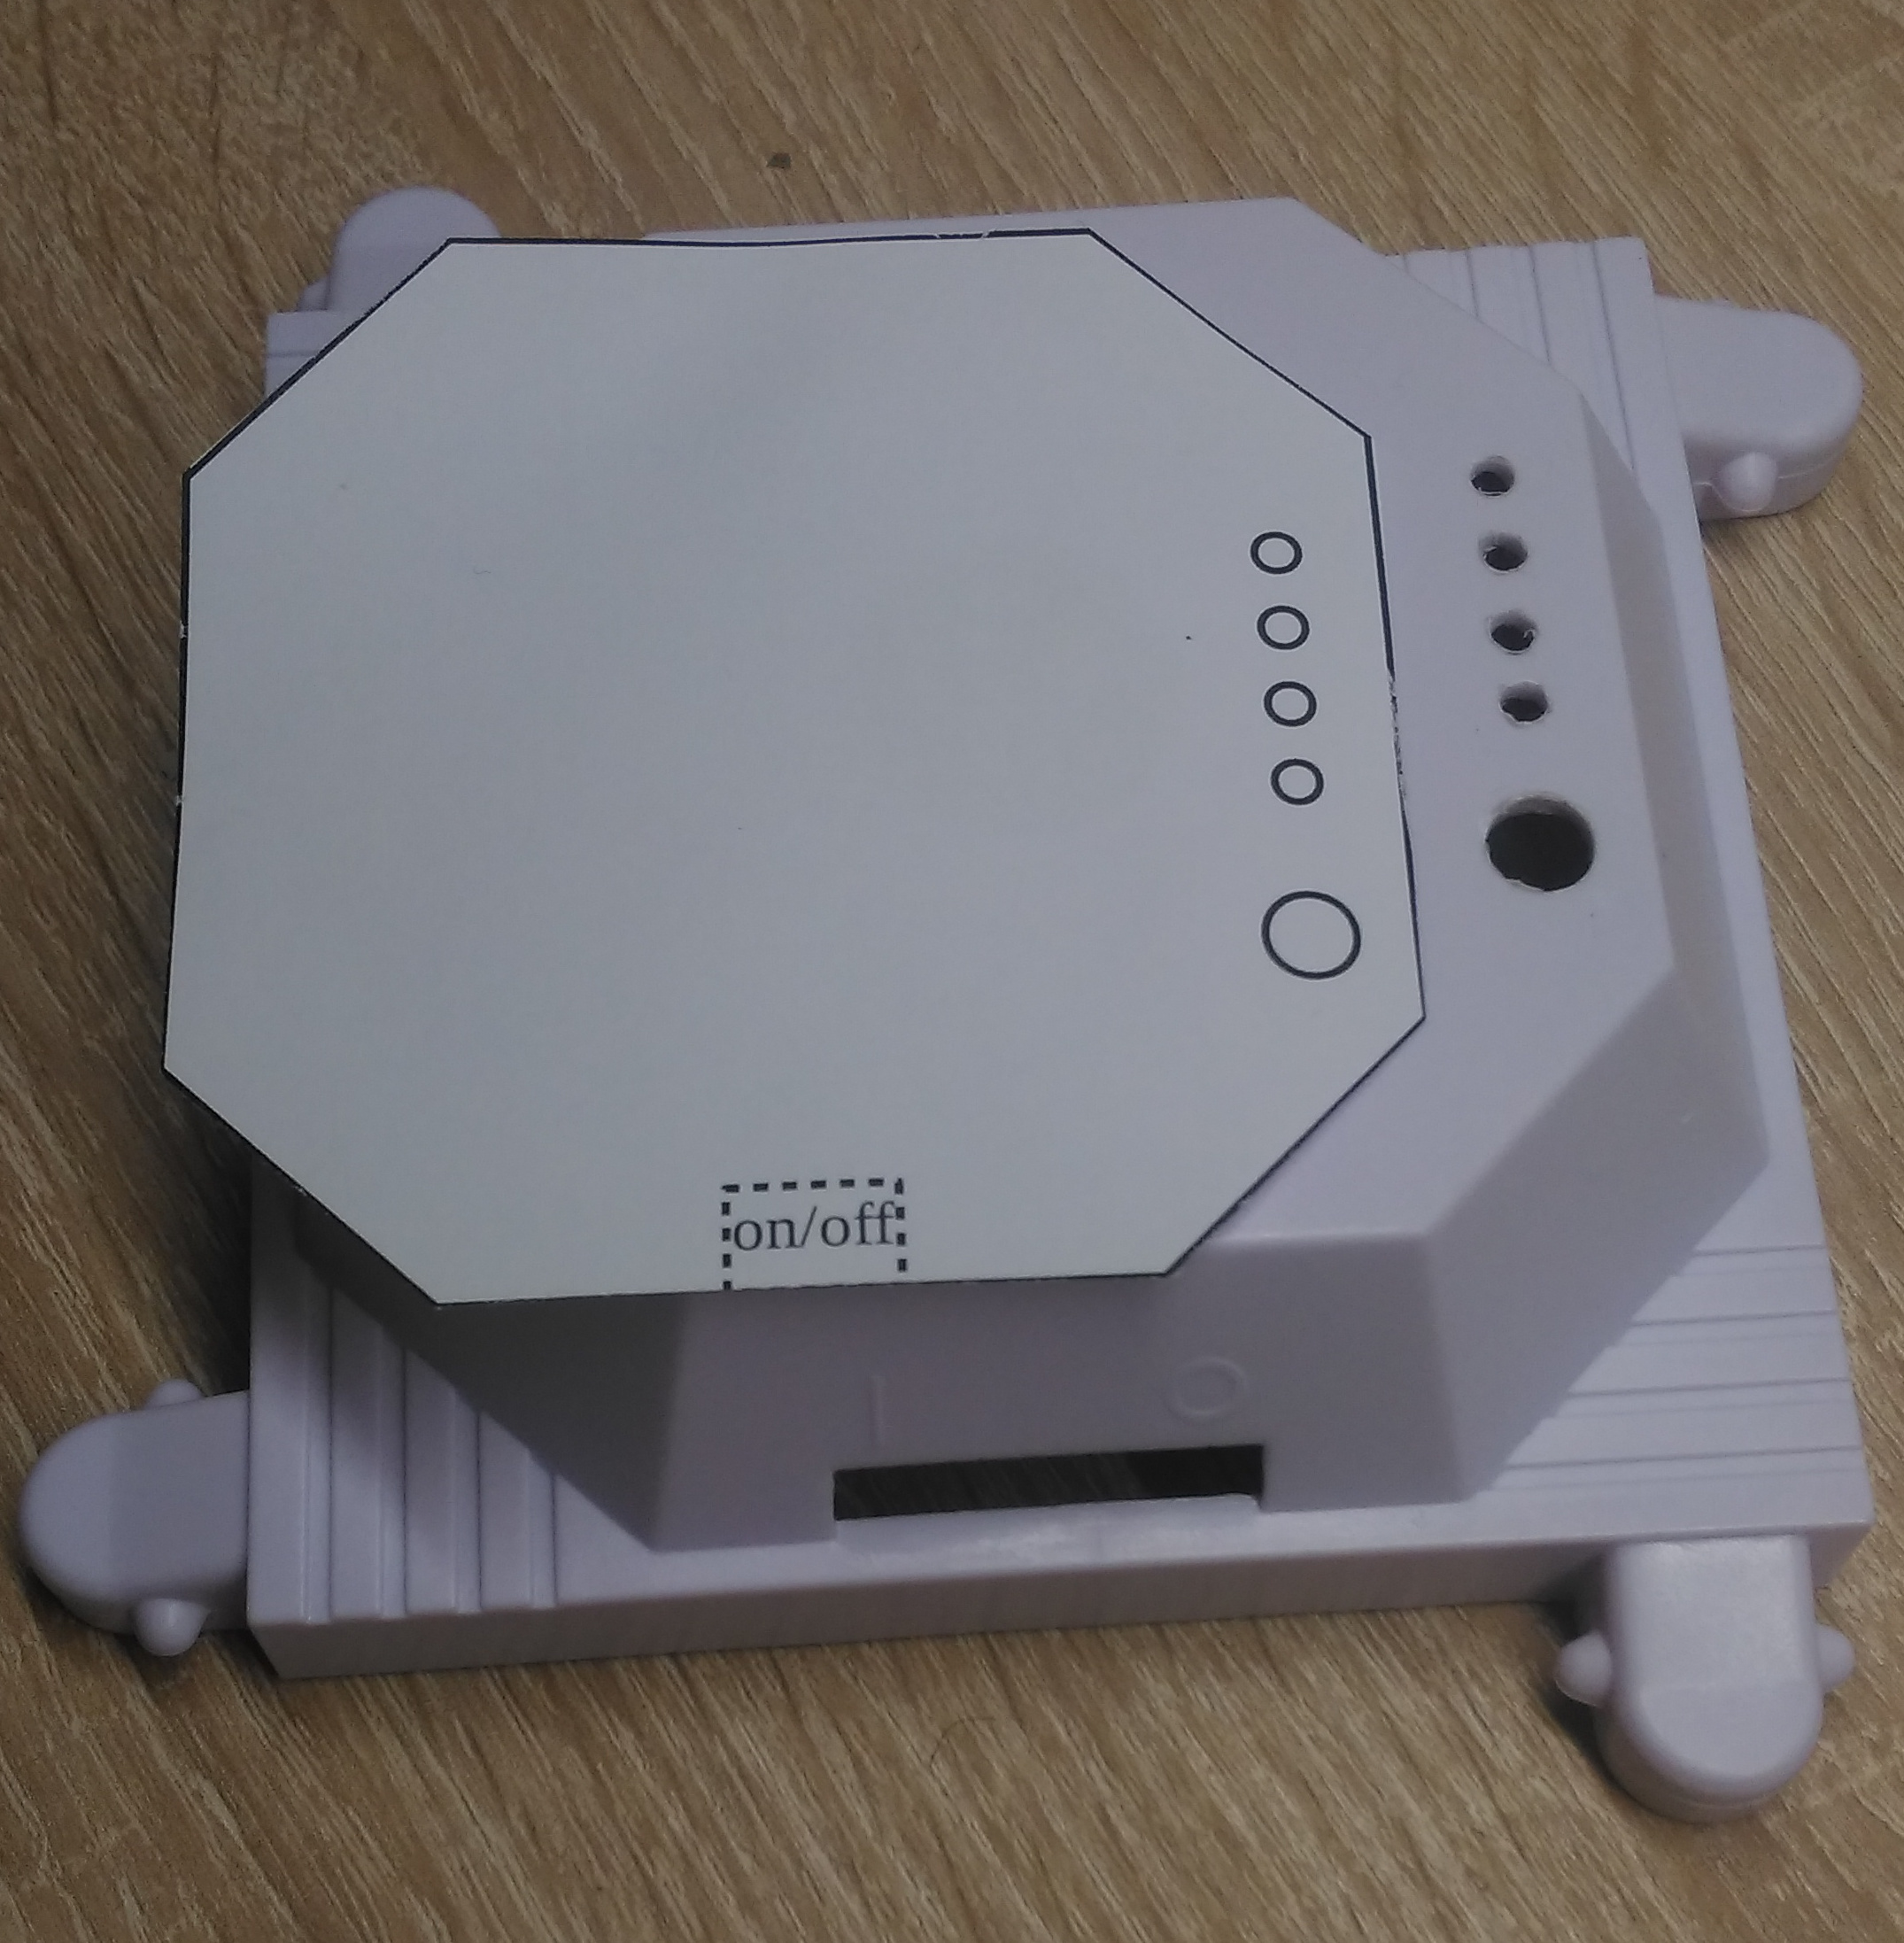
\includegraphics[width=0.5\textwidth]{pictures/loolou_013.jpg}
	\centering
	\caption{Spielbasis - Gebohrte L"ocher f"ur die LEDs und den Taster im Oberteil}
	\label{fig13}
\end{figure}
\vspace{0.5cm}
\newpage

Nun nimmt man das kleine Rechteckige Teil der Schablone und k"ornt damit an jeder der 4 Seiten das Loch f"ur die 5mm gro"sen LEDs an (Kreis mit durchgezogener Linie). Dabei muss der Kreis mit der durchgezogenen Linie zu dem Verbindungsstück, für die Arme des Looping Louie, zeigen (zu sehen in Abbildung ~\ref{fig14}). Der gestrichelte Kreis ist f"ur den Stromanschluss. Dieser wird auf der gegeb"uberliegenden Seite des AN/AUS-Schalters gebohrt (zu sehen in Abbildung ~\ref{fig14}). Die L"ocher f"ur die LEDs werden mit einem Bohrer der St"arke von 5mm und das Loch f"ur den Stromanschluss mit einen 7mm gro"sen Bohrer gebohrt.  

\vspace{1cm}
\begin{figure}[!ht]
	\centering
  	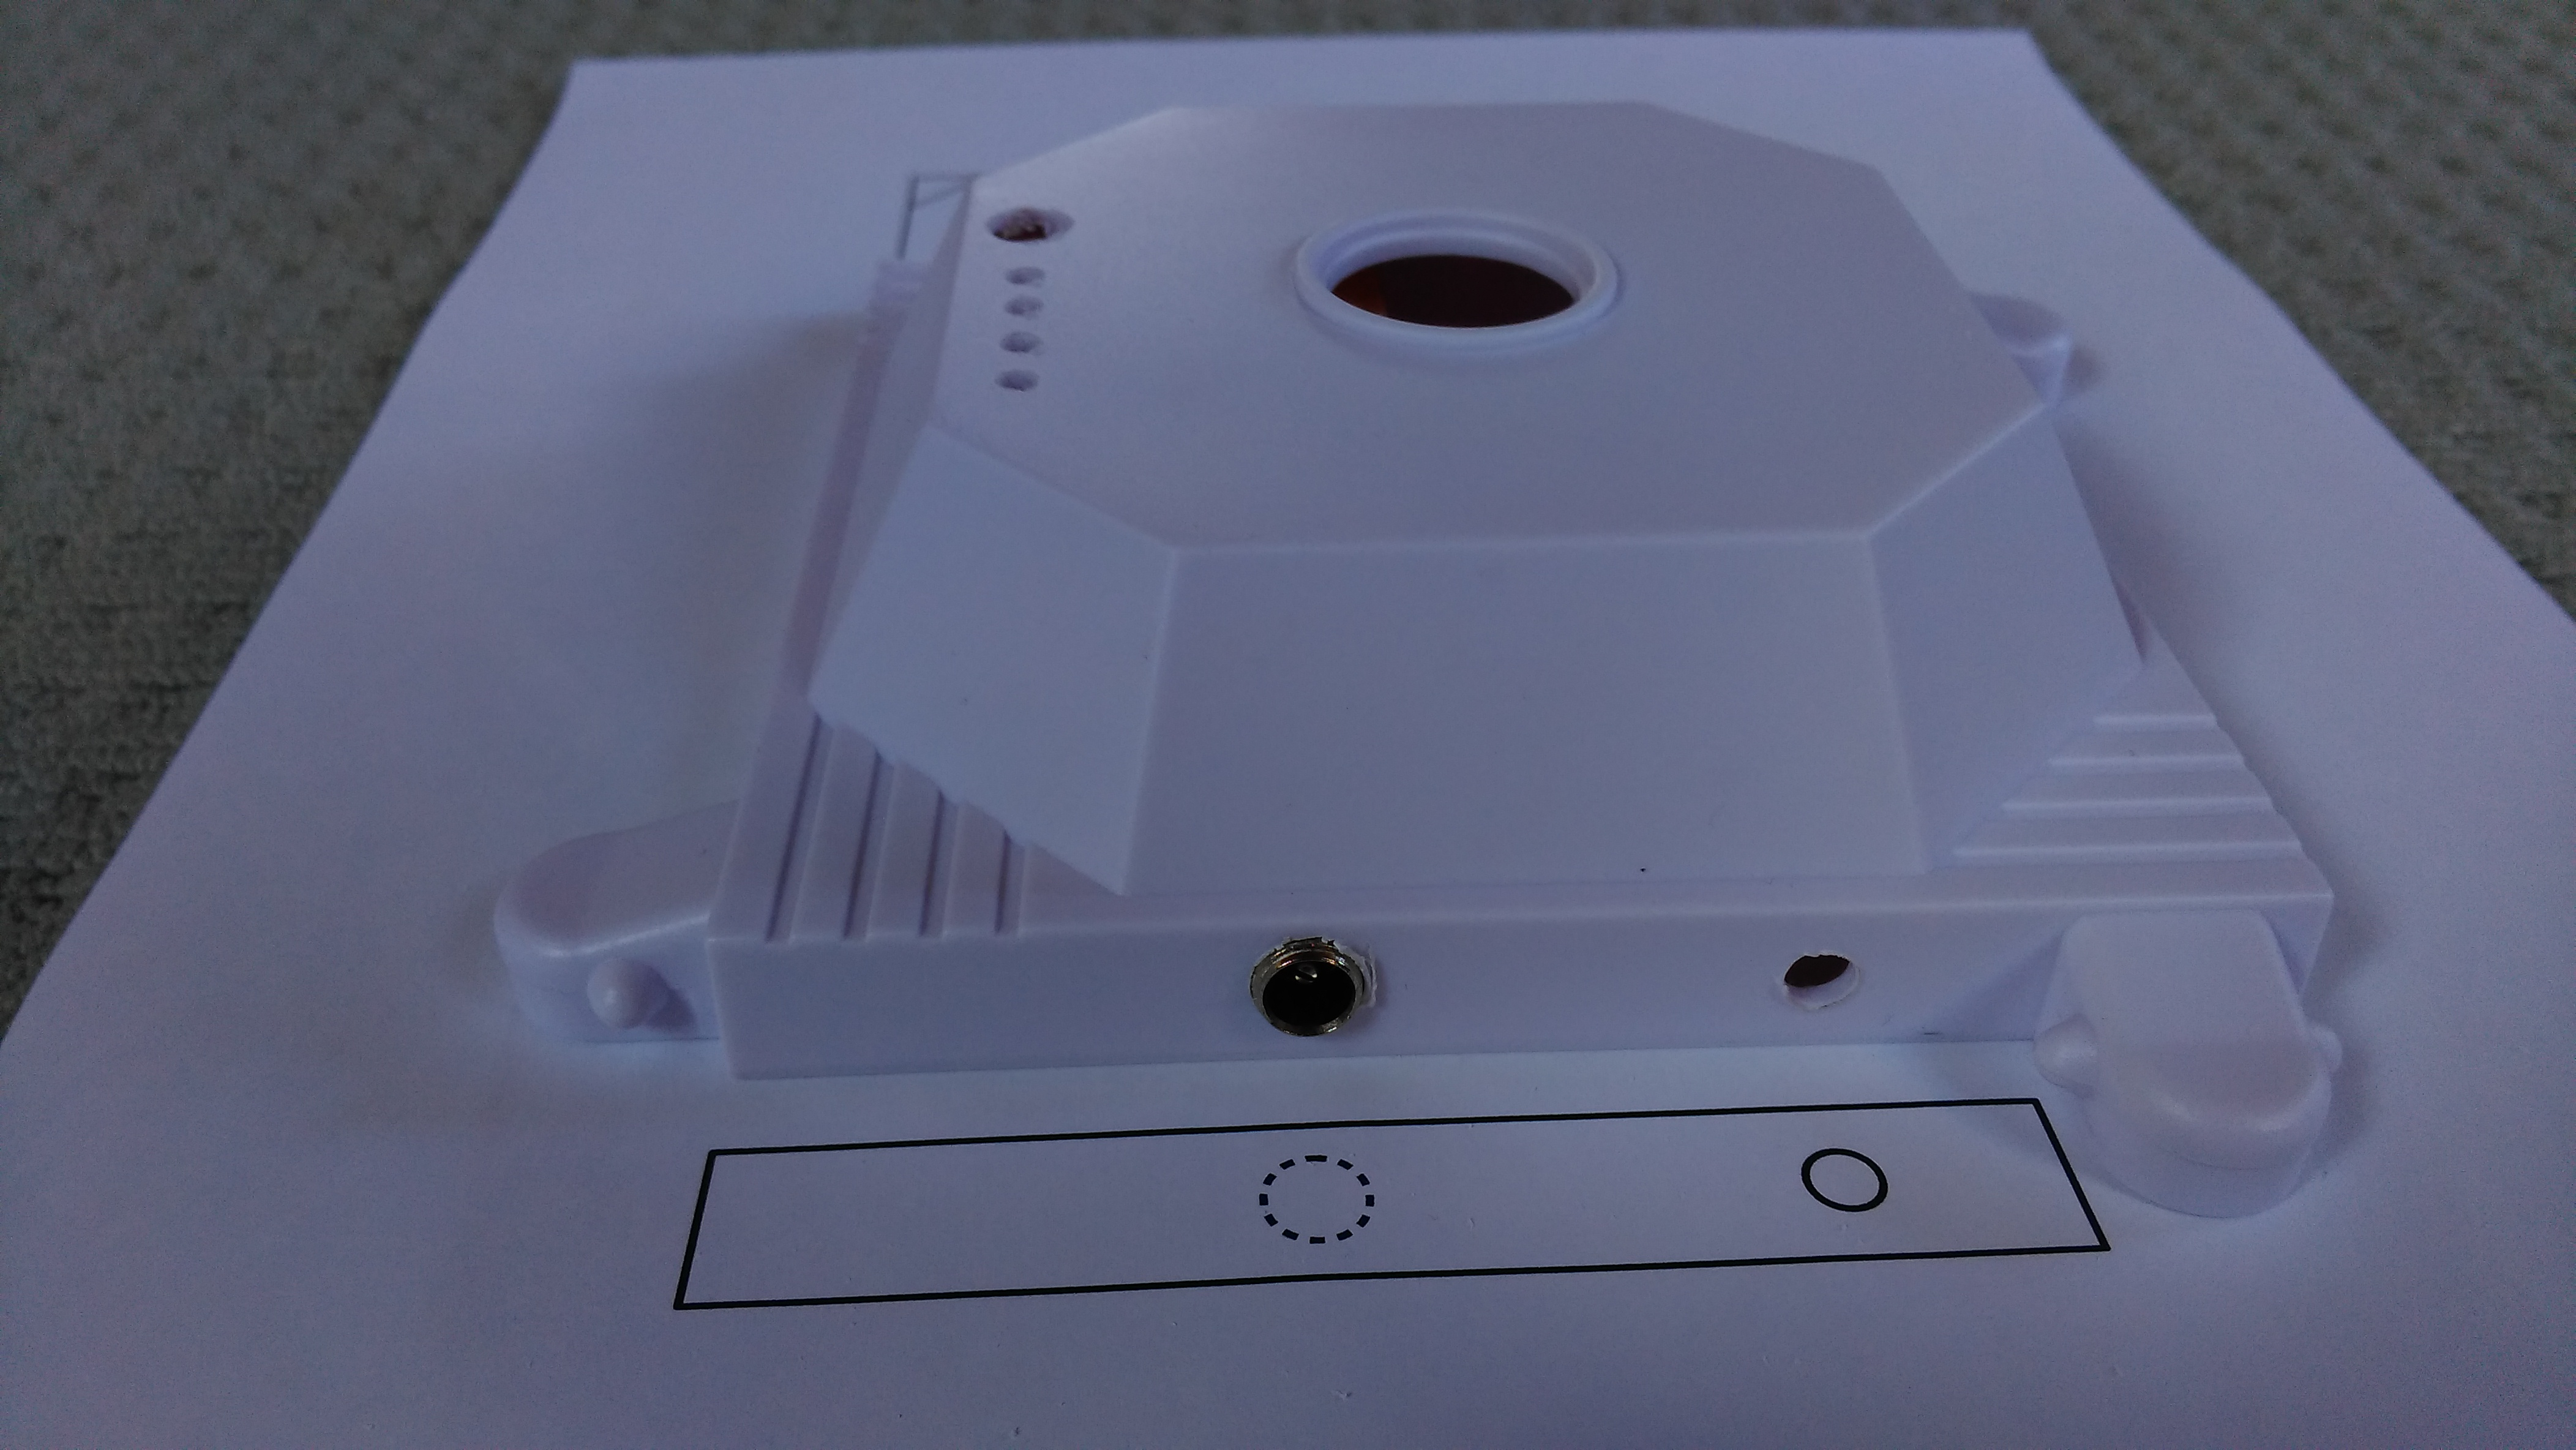
\includegraphics[width=0.7\textwidth]{pictures/loolou_014.jpg}
	\caption{Spielbasis - Mit gebohrte L"ocher in der Seite des Oberteils}
	\label{fig14}
\end{figure}
\vspace{0.5cm}

Zum Abschluss k"onnen nun noch alle LEDs, der Drucktaster und der Stromanschluss in die Spielbasis gesteckt werden. Sollte hier noch etwas klemmen kann an dieser Stelle noch leicht nachgearbeitet werden.

\vspace{1cm}
\begin{figure}[!ht]
	\centering
  	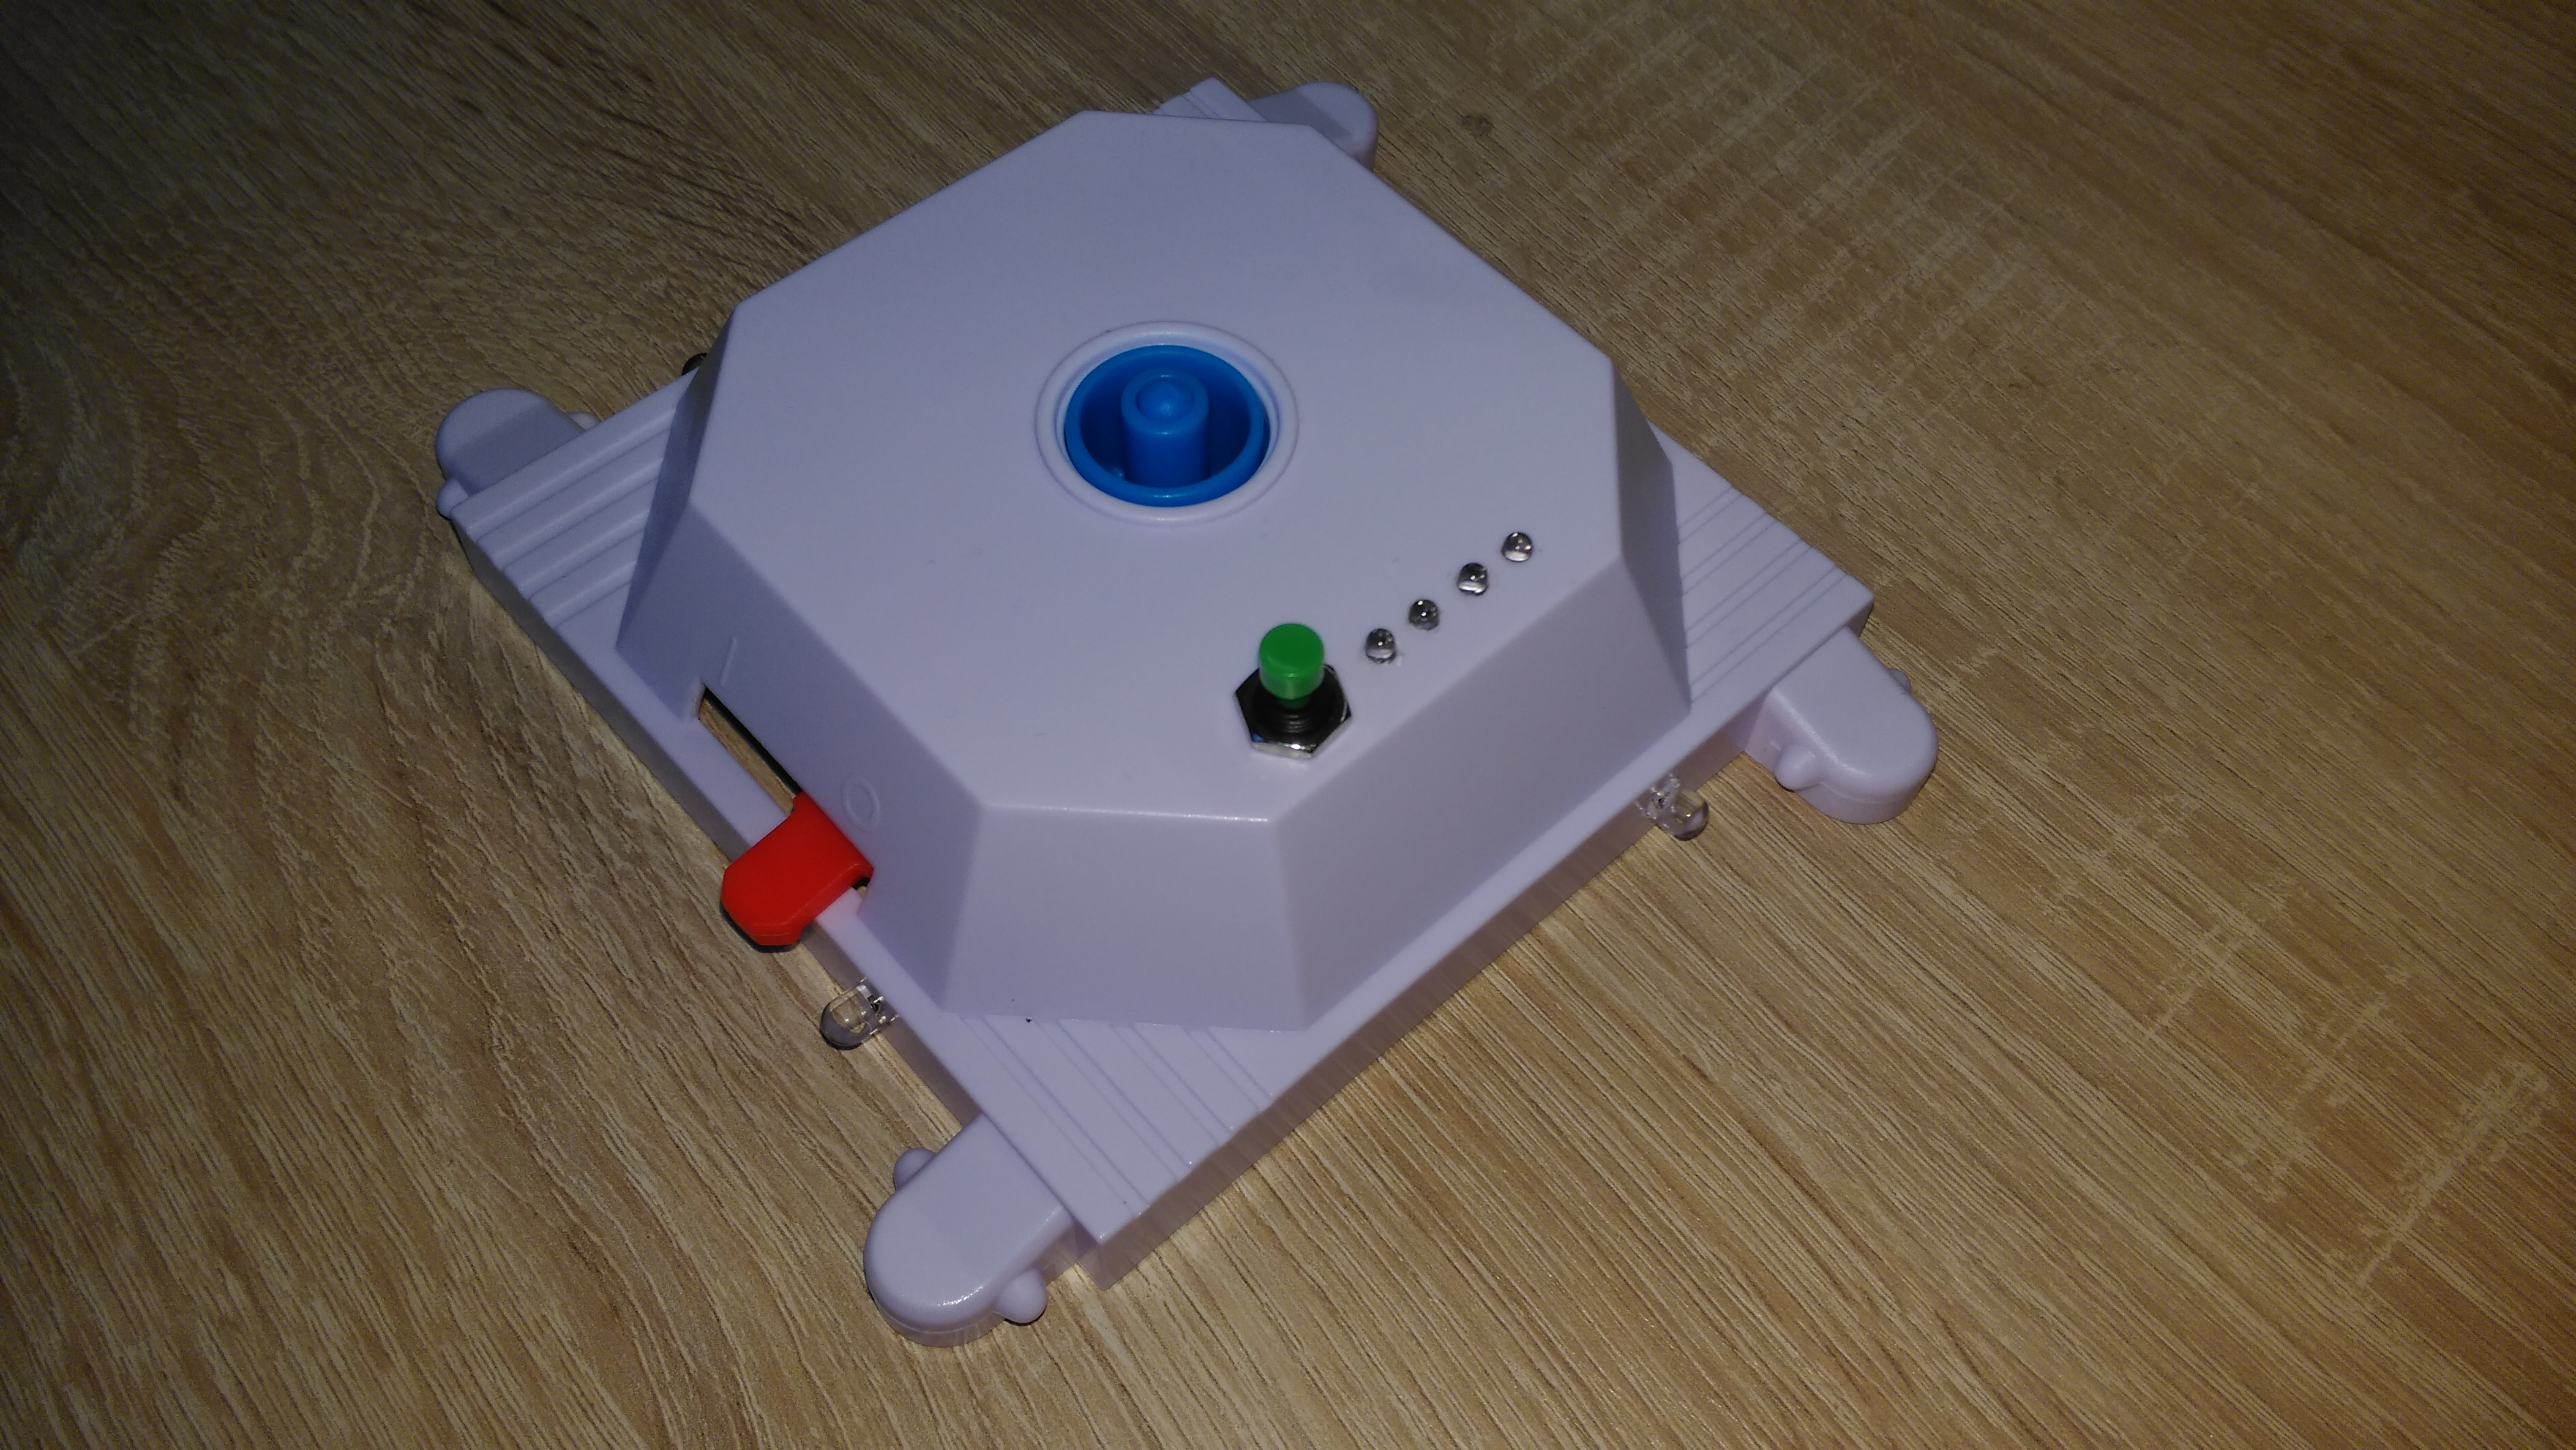
\includegraphics[width=0.7\textwidth]{pictures/loolou_015.jpg}
	\caption{Spielbasis - Mit gesteckten LEDs, dem Drucktaster und dem Stromanschluss}
	\label{fig15}
\end{figure}
\vspace{0.5cm}

Die Abbildung ~\ref{fig15} zeigt die Spielbasis mit den gesteckten LEDs, dem Drucktaster und dem Stromanschluss. 


\newpage
\subsection{Platine}

Nun widmen wir uns der Platine - dem Herzst"uck der Erweiterung von Looping Louie. Zu sehen ist diese in den Abbildungen ~\ref{fig16} (a) und (b).

\vspace{1cm}
\begin{figure}[!ht]
	\centering
  	\subfigure[Oberseite]{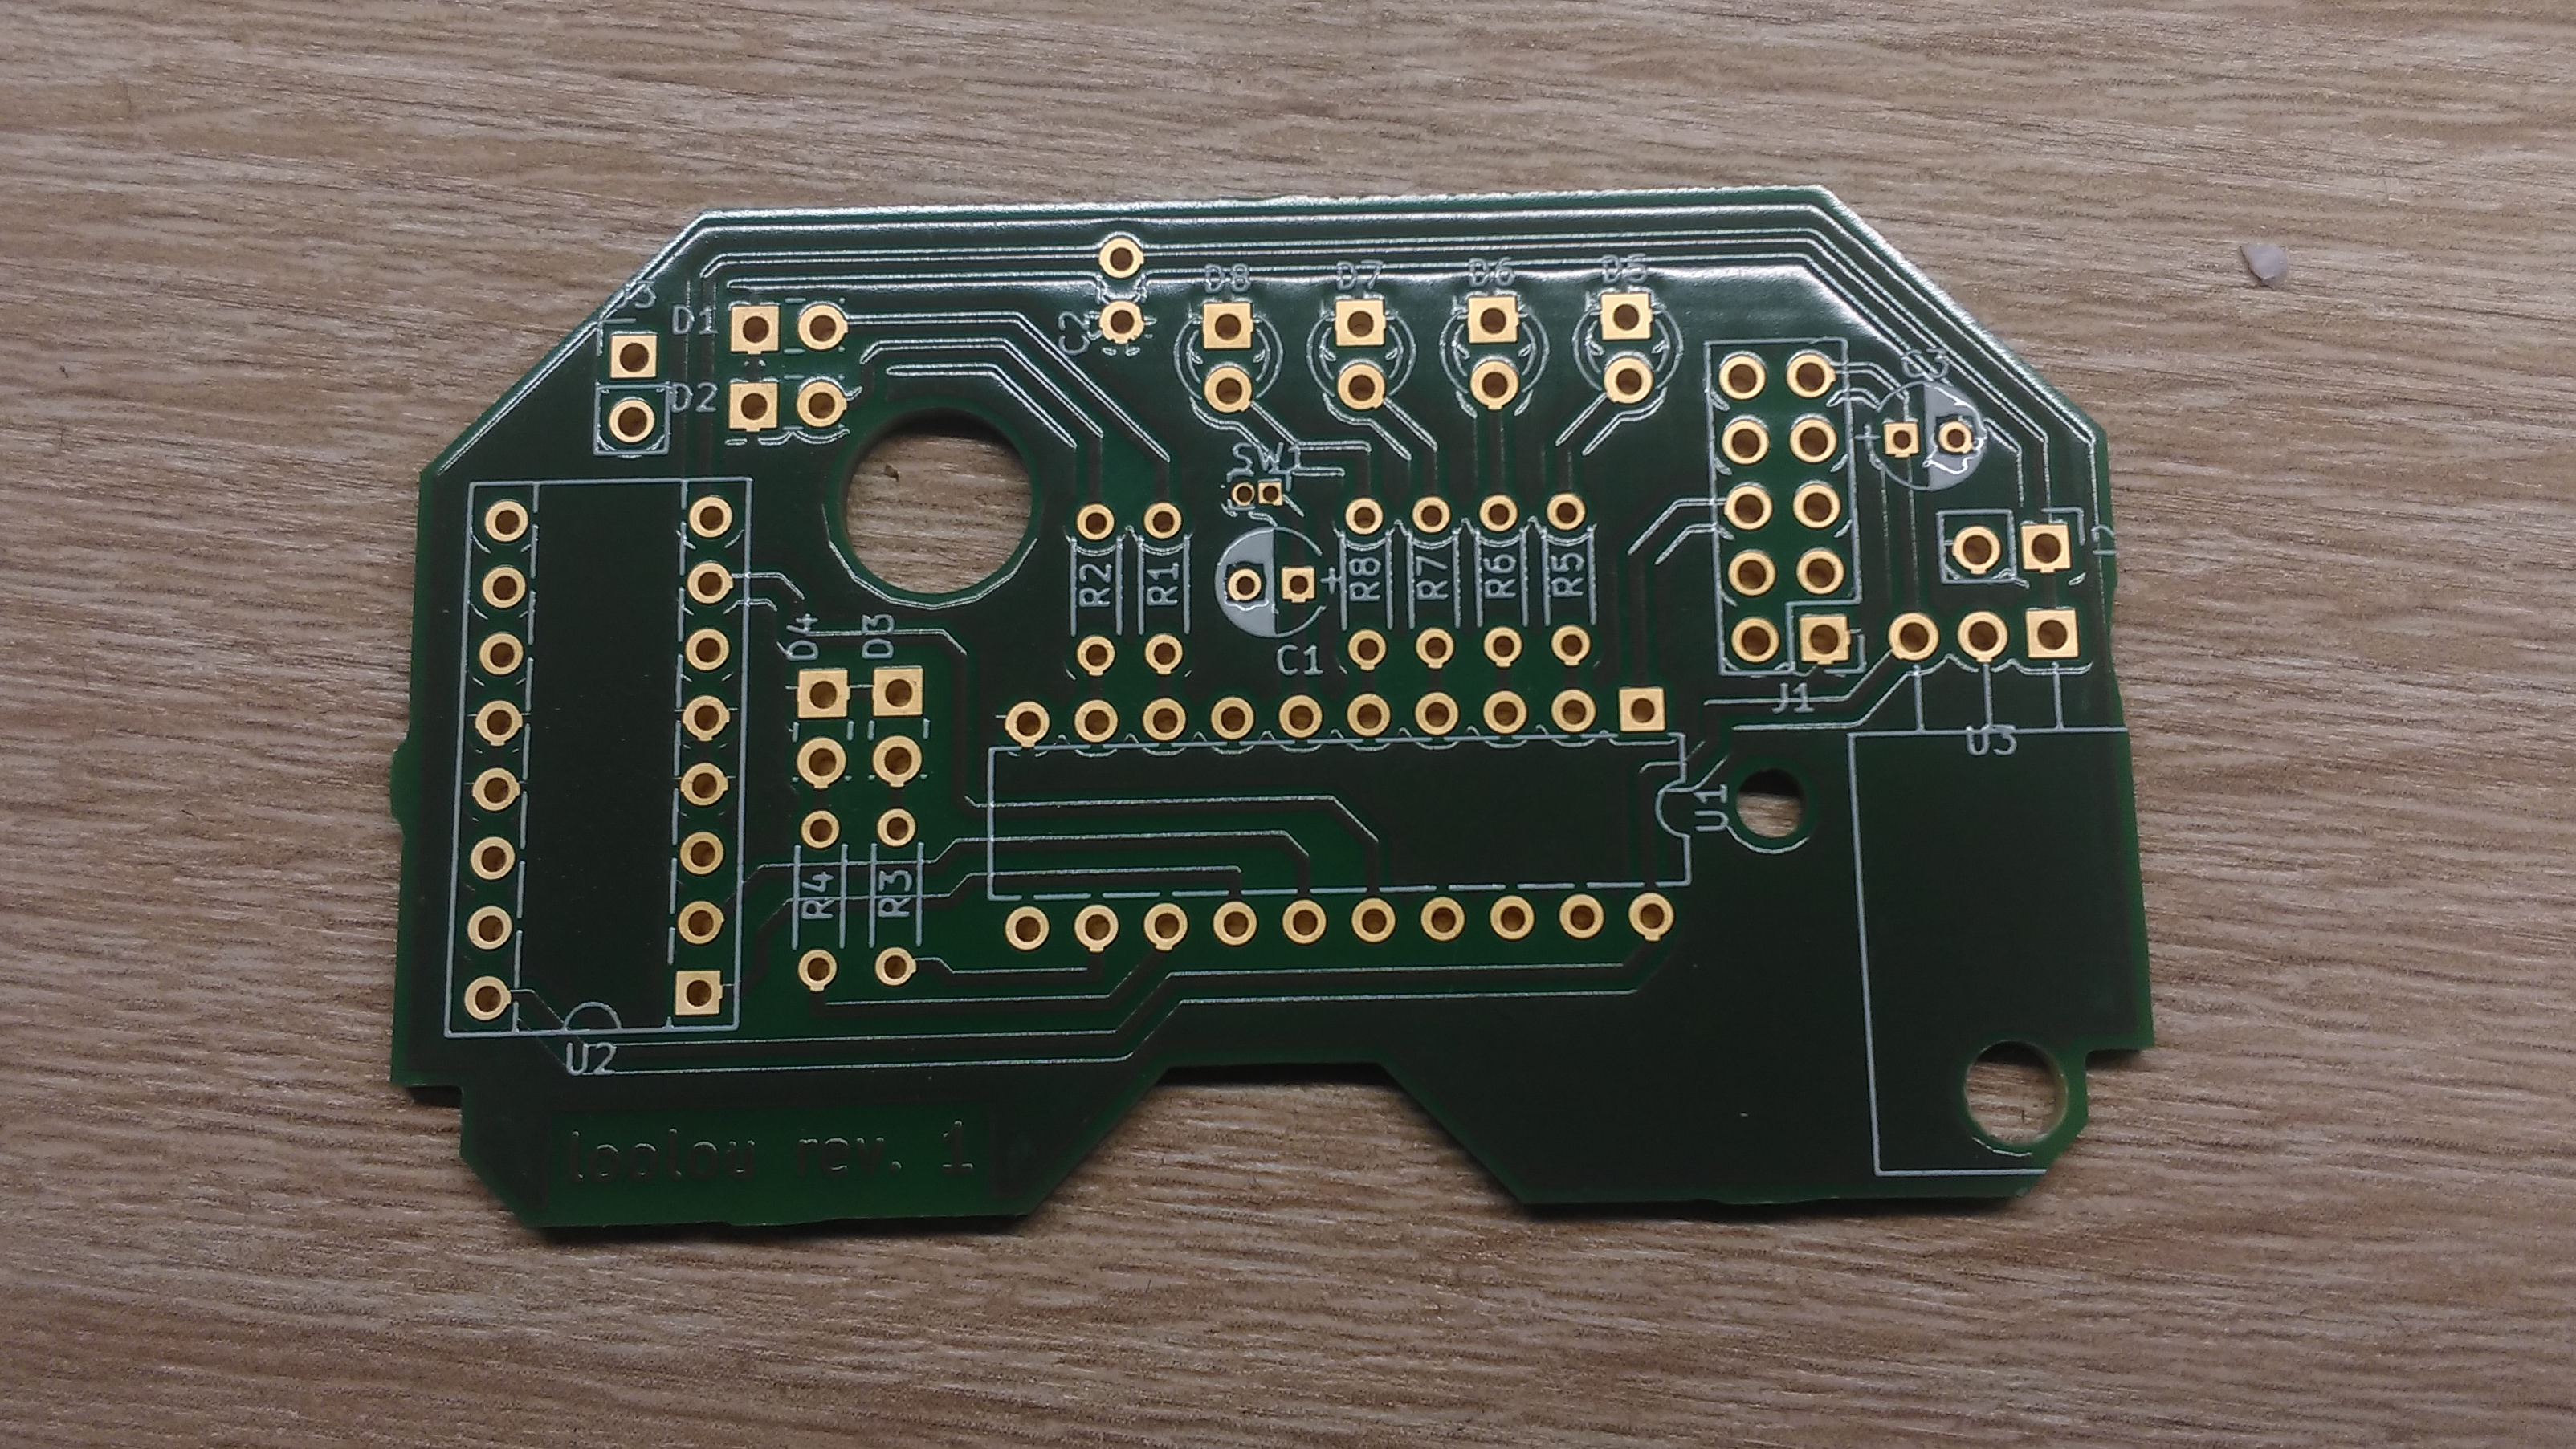
\includegraphics[width=0.49\textwidth]{pictures/loolou_016.jpg}}
	\subfigure[Unterseite]{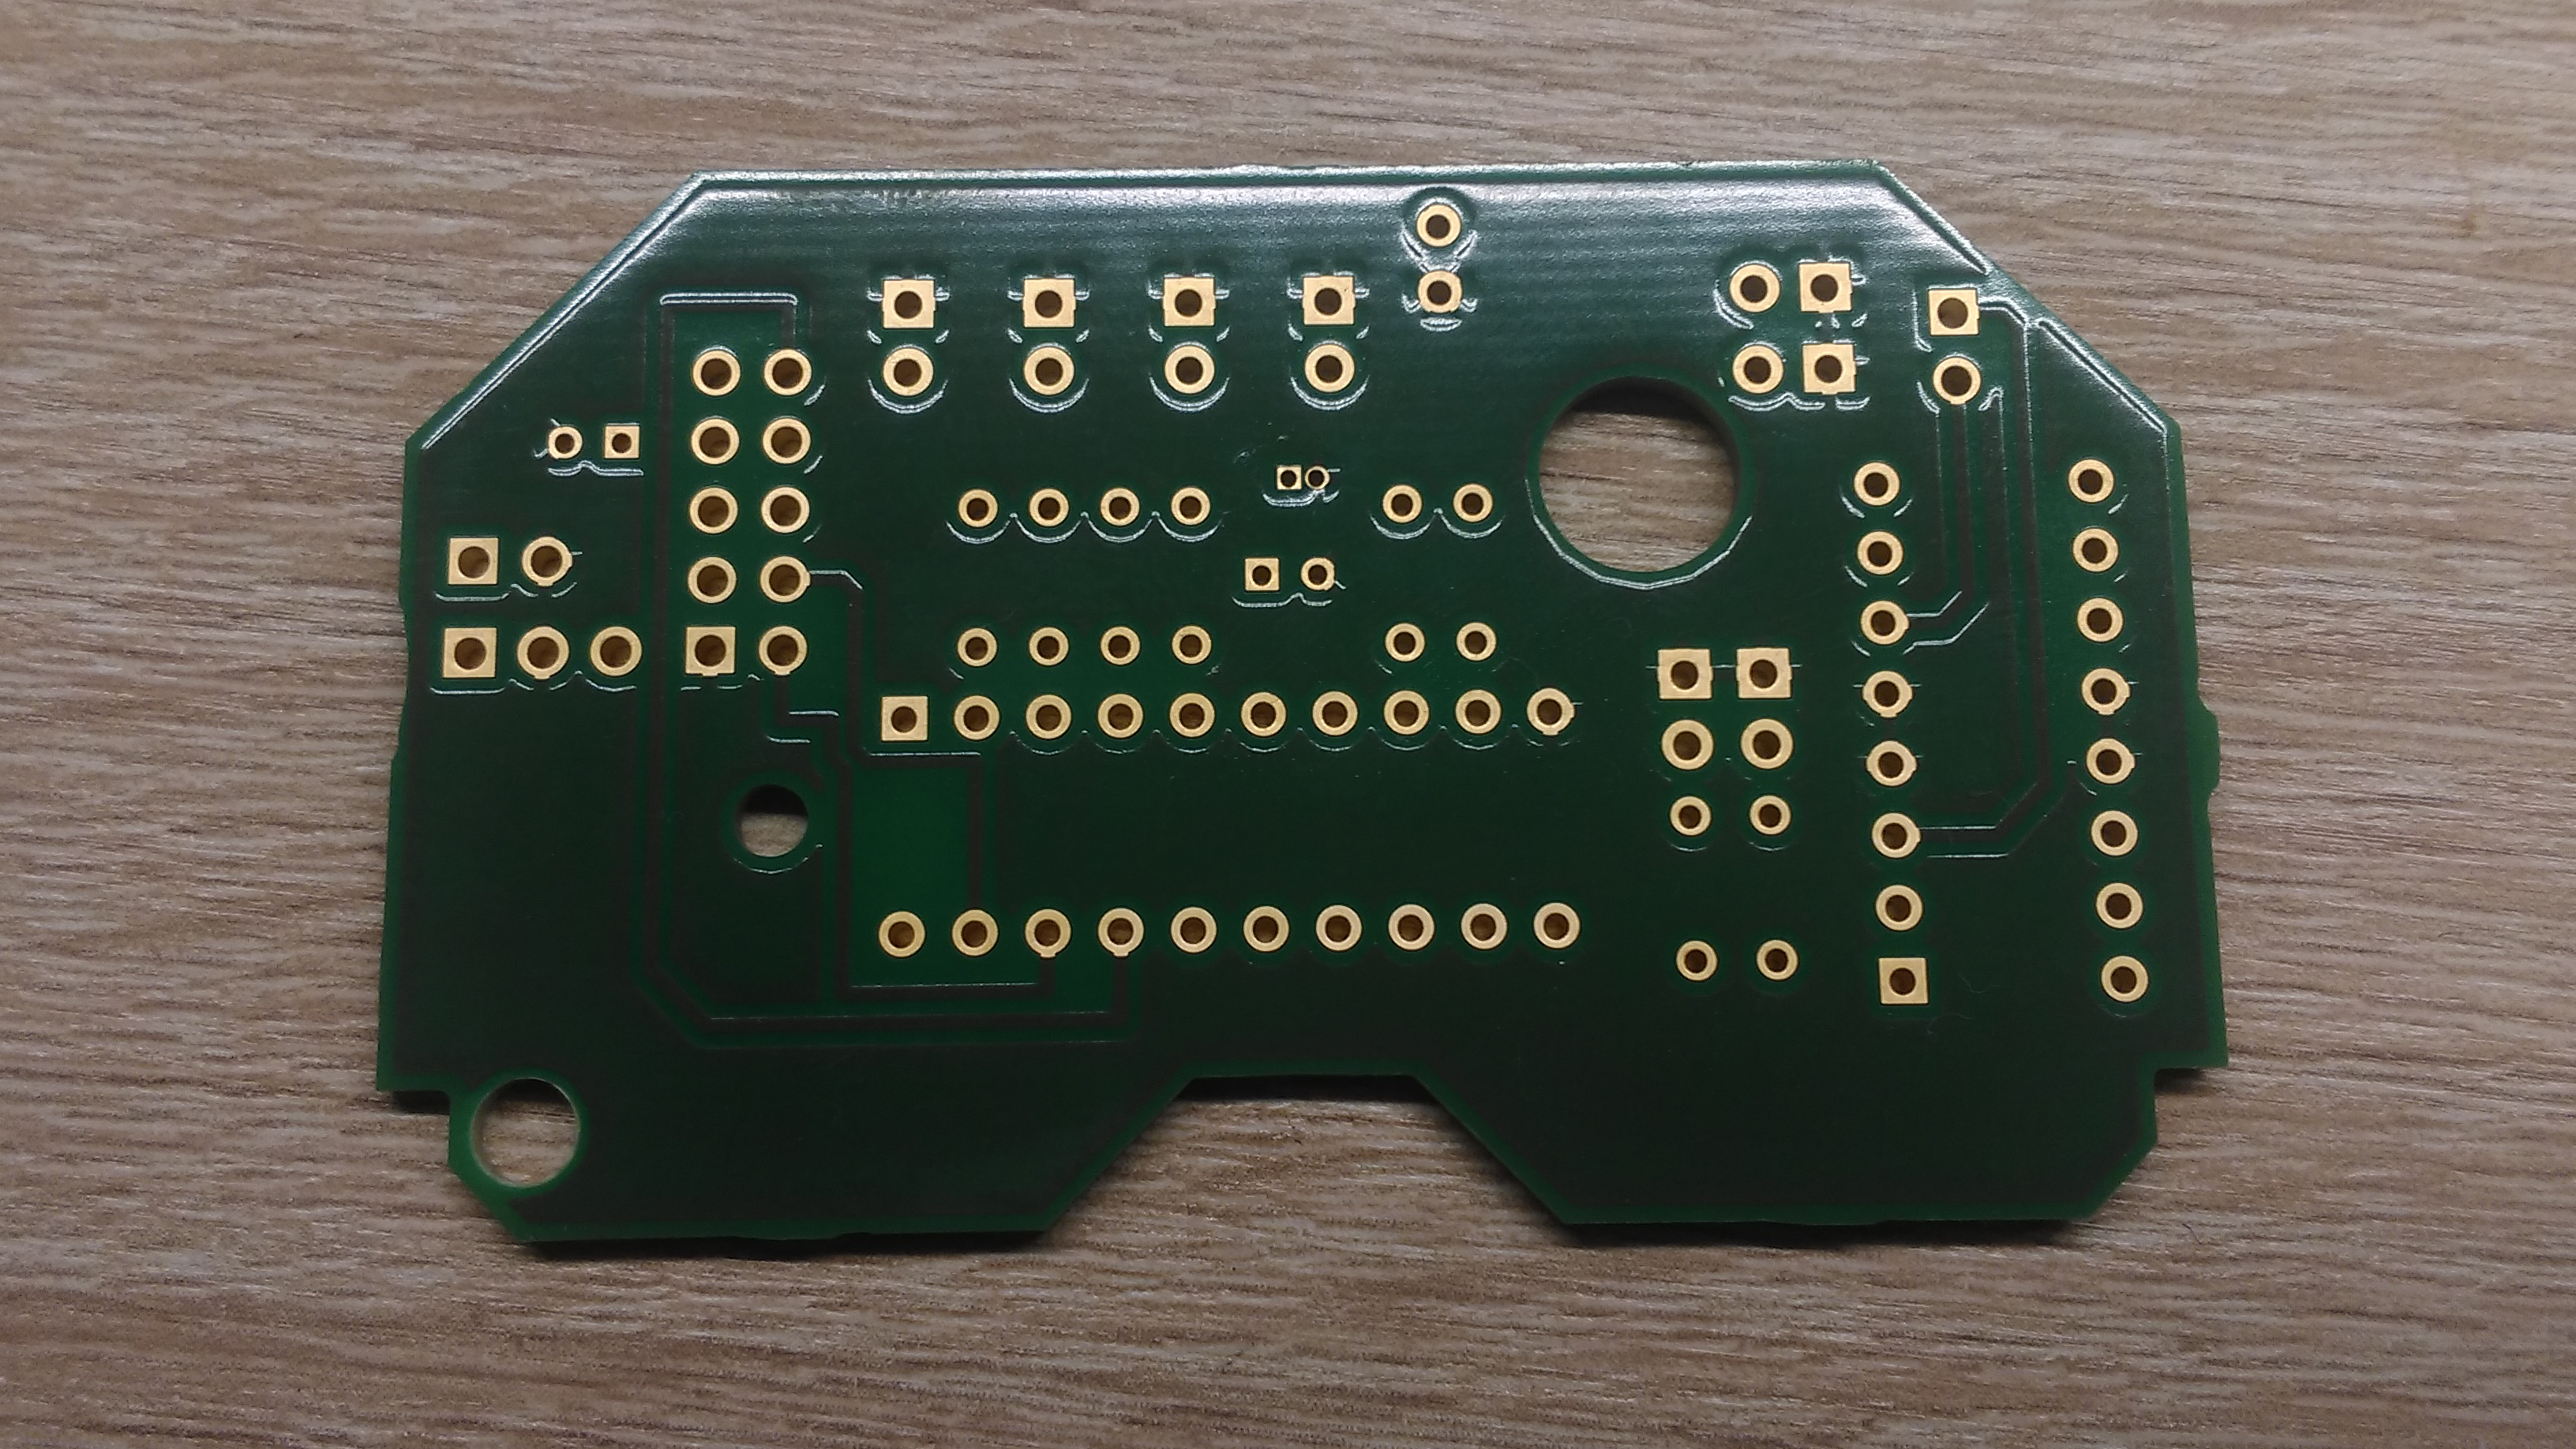
\includegraphics[width=0.49\textwidth]{pictures/loolou_017.jpg}}
	\caption{Originale Platine - Revision 1}
	\label{fig16}
	%\label{fig17}
\end{figure}
\vspace{0.5cm}

Auf der Platine sind unteranderem ein kleiner Microcontroller (ATTINY2313), ein Treiberbaustein, ein Festspannungsregler sowie diverse LEDs und Widerst"ande verbaut. Der Schaltplan ~\ref{appendix2} und das Platinen-Layout ~\ref{appendix3} kann im Anhang gefunden werden. Die Referenzen der Bauteile k"onnen der Tabelle ~\ref{table:components} entnommen werden.  \\
\\
Am einfachsten beginnt man an dieser Stelle mit den IC-Sockeln (U1 und U2), sowie dem Festspannungsregler (U3). Im Anschluss kann der 10polige Wannenstecker (J1), f"ur den Programmer, aufgel"otet werden, dieser ist Optional und wird nur ben"otigt wenn man den Attiny zum programmieren nicht herausnehmen m"ochte.
Nachdem die IC-Sockel und der Festspannungsregler aufgel"otet wurden, k"onnen die Widerst"ande (R1-R8) und die Kondensatoren (C1-C3) aufgel"otet werden.
Die Abbildung ~\ref{fig18} zeigt die Platinen nach dem aufl"oten der Widerst"ande, der Kondensatoren, dem Festspannungsregler und den IC-Sockeln.

\vspace{1cm}
\begin{figure}[!ht]
	\centering
  	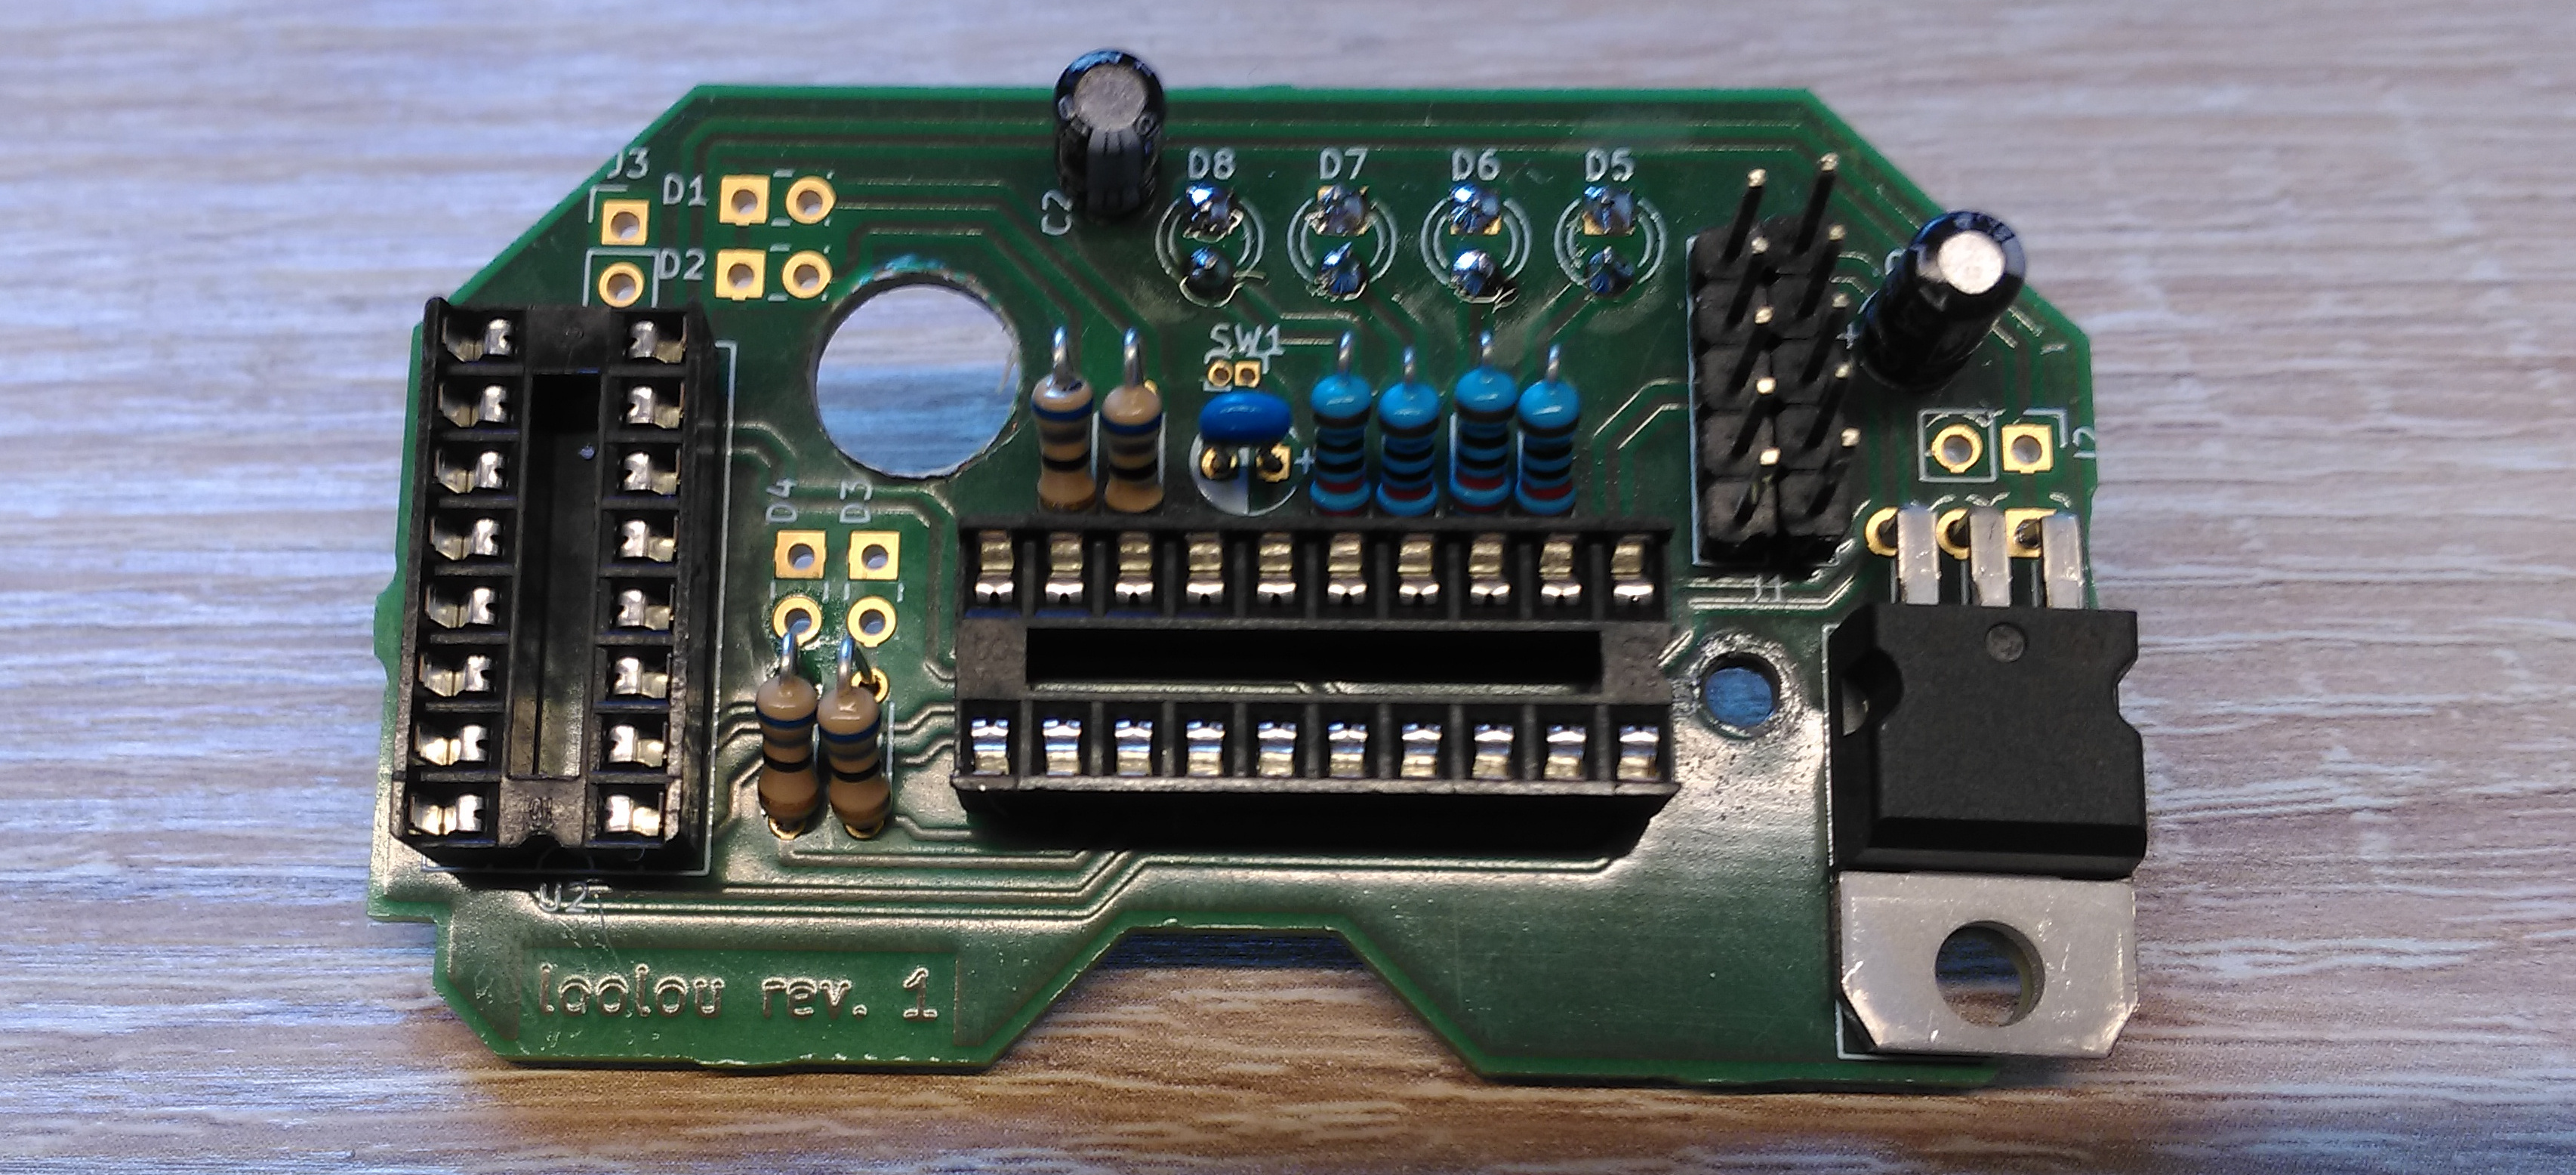
\includegraphics[width=0.7\textwidth]{pictures/loolou_018.jpg}
	\caption{Platine mit aufgel"oteten Widerst"anden und IC-Sockel}
	\label{fig18}
\end{figure}
\vspace{0.5cm}

Nachdem nun die IC-Sockel (U1,U2), der Festspannungsregler (U3), die Widerst"ande (R1-R8) und die Kondensatoren (C1-C3) aufgel"otet wurden, sollten die LEDs (D5-D8) aufgel"otet werden. Dazu steckt man diese einzeln, von innen, in das Oberteil der Spielbasis und schraubt dann die Platine in den daf"ur vorgesehenen Platz im Oberteil der Spielbasis. Wie die Platine in das Oberteil der Spielbasis geschraubt wird zeigt die Abbildung ~\ref{fig19} \\
Nachdem nun die LEDs in die Spielbasis gesteckt und die Dr"ahte der LEDs (D5-D8) durch die daf"ur vorgsehenen L"ocher gef"uhrt wurden, k"onnen diese an der Platine festgel"otet werden. Achte an dieser Stelle darauf das die LEDs richtig gepolt sind, ansonsten m"ussen diese sp"ater wieder entfernt und neu aufgel"otet werden.
% TODO Es ist einfacher wenn alle LEDs einzeln eingescteckt weren -> LED5 rein, festscahrauben, lötem, rasuschrauben -> nächste LED  

\vspace{1cm}
\begin{figure}[!ht]
	\centering
  	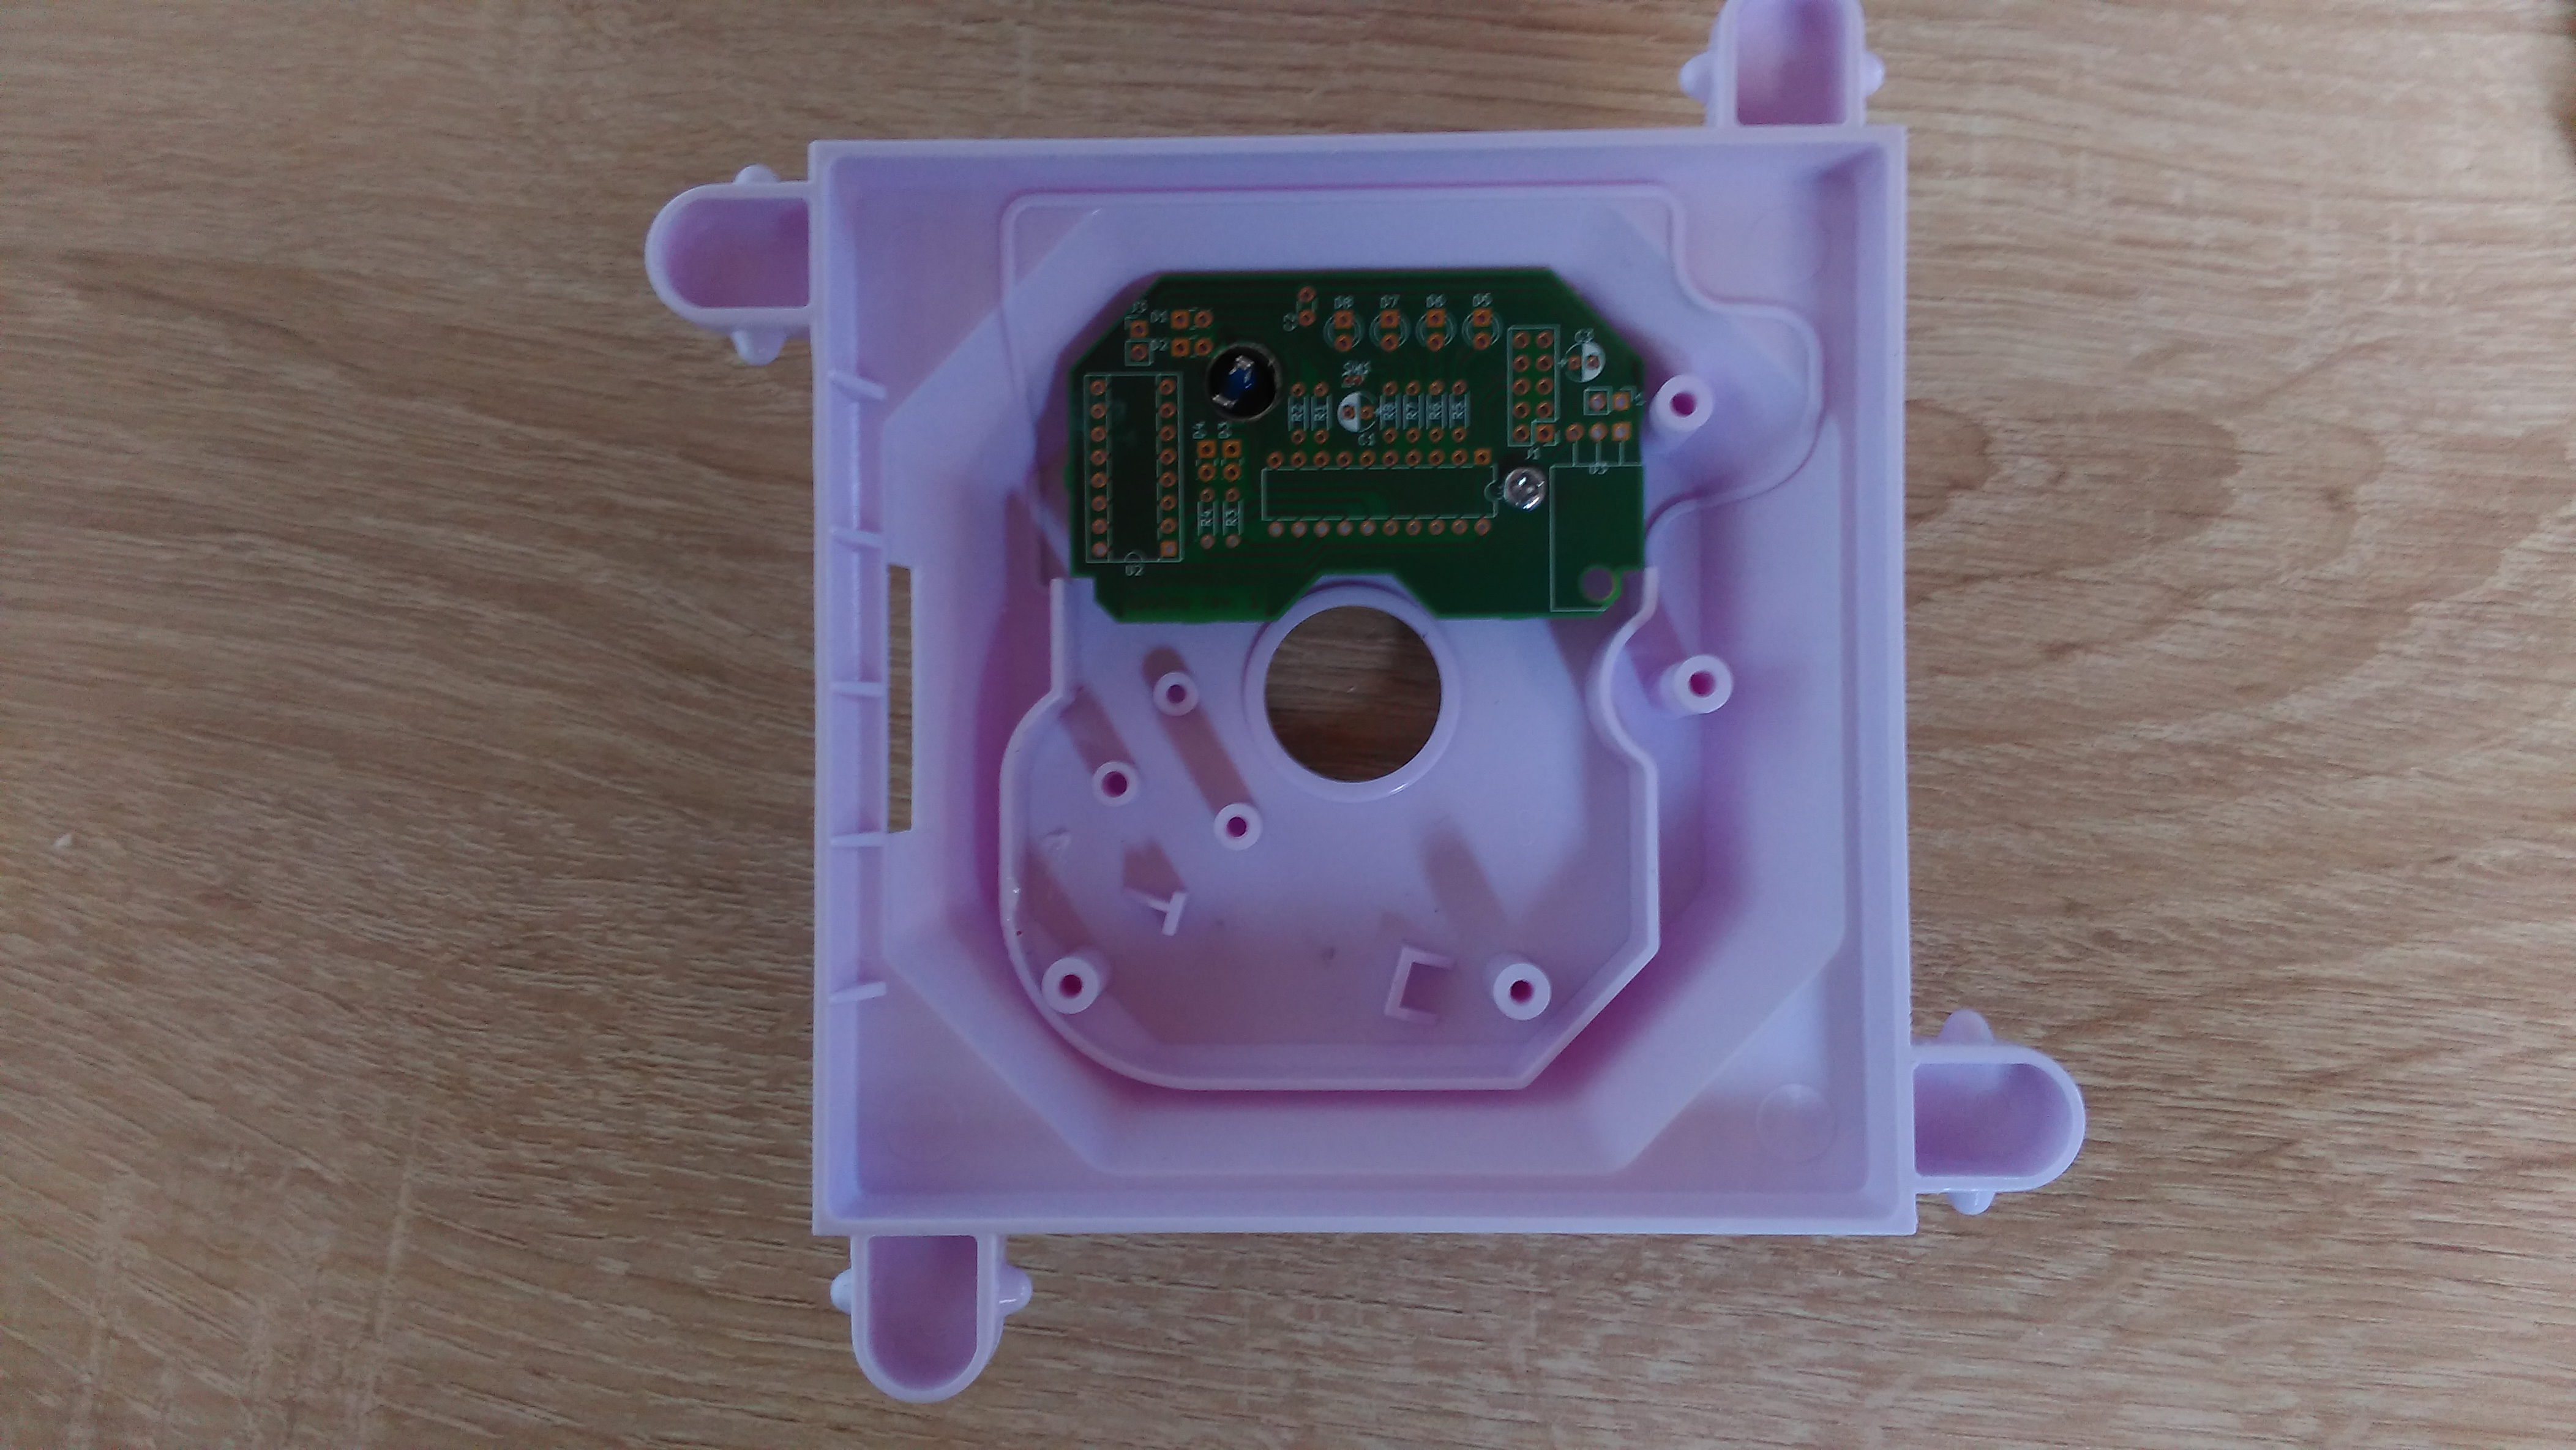
\includegraphics[width=0.7\textwidth]{pictures/loolou_019.jpg}
	\caption{Platine festgeschraubt im Oberteil der Spielbasis}
	\label{fig19}
\end{figure}
\vspace{0.5cm}

Nachdem nun auch die LEDs D5 bis D8 aufgel"otet sind kann die Platine nun wieder aus der Spielbasis herausgenommen werden. Die Abbildung ~\ref{fig20} zeigt die Platine mit den festgel"oteten LEDs (D5-D8). \\
Es empfiehlt sich an dieser Stelle die bisher festgel"oteten Bauteile und die L"otstellen mit einem Durchgangspr"ufer zu testen, um kalte L"otstellen und verpolte LEDs rechtzeitig zu erkennen.

\vspace{1cm}
\begin{figure}[!ht]
	\centering
  	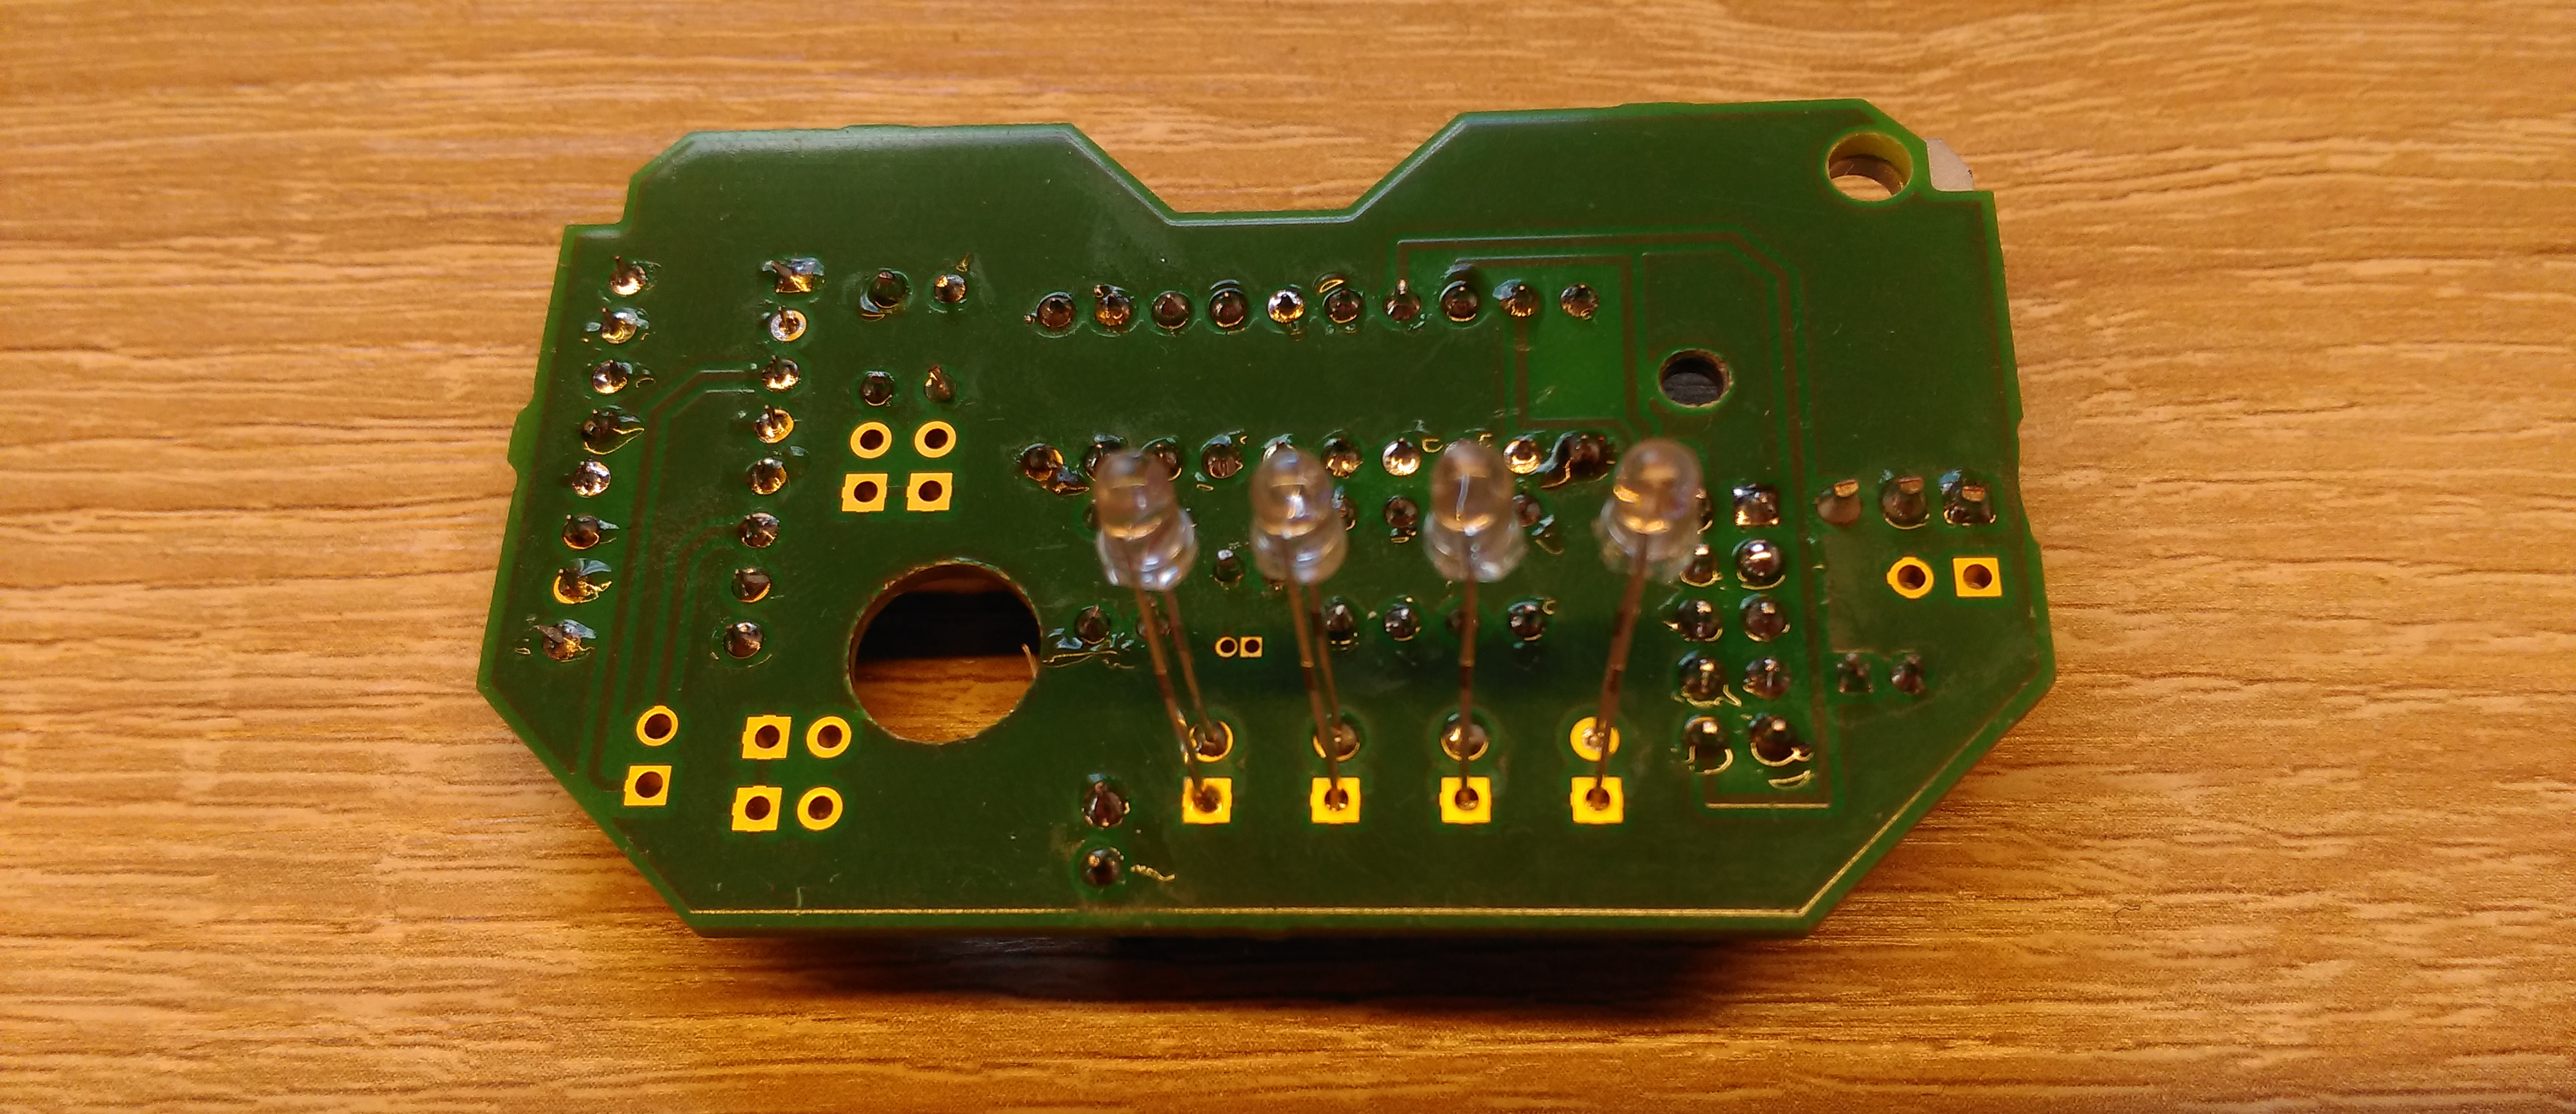
\includegraphics[width=0.7\textwidth]{pictures/loolou_020.jpg}
	\caption{Platine mit LEDs auf der Unterseite}
	\label{fig20}
\end{figure}
\vspace{0.5cm}

An dieser Stelle sollten die Litzen f"ur die restlichen LEDs (D1-D4), den Drucktaster (SW1), den Hohlstecker-Buchse (J2) und den Motor vorbereitet werden. Die L"ange der Litzen kann einfach der Tabelle ~\ref{table:cable} entnommen werden. Es werden jeweils eine rote und eine schwarze Litze ben"otigt.

\vspace{1cm}
\begin{table}[ht]
	\centering

	\begin{tabular}{ | l | l | l | } 
		\hline % table header
		Reference	& Description		& Length \\ 
		\hline \hline
		D1		& LED1, 5mm		& 9cm  \\
		\hline
		D2		& LED2, 5mm		& 13cm \\
		\hline
		D3		& LED3, 5mm		& 13cm \\
		\hline
		D4		& LED4, 5mm		& 13cm \\
		\hline
		SW1		& Drucktaster		& 5cm  \\
		\hline
		J1		& Hohlstecker-Buchse	& 7cm  \\
		\hline
		J3		& Motor			& 16cm \\
		\hline
	\end{tabular}

	\caption{Litzenl"ange}
	\label{table:cable}
\end{table}
\vspace{0.5cm}

Sobald diese vorbereitet wurden, können die Litzen bereits an die LEDs (D1-D4) gel"otet werden. Dazu schneidet man am Besten die Dr"ahte der LEDs auf einen Zentimeter herunter und l"odet dann die Kabel an. Im Anschluss sollten noch die offenen L"otstellen mit einem Schrumpfschlauch verschlossen werden. Anschlie"send k"onnen auch die Litzen an den Drucktaster und die Hochstecker-Buchse gel"otet und mit einem Schrumpfschlauch verschlossen werden. \\
Das Pin-Layout, der Hohlstecker-Buchse, kann dem Datenblatt entnommen werden. FÜr die Hohlstecker-Buchse \grqq HEBL 21\grqq  (\href{https://www.reichelt.com}{www.reichelt.com}) ist das Pin-Layout in der Abbildung ~\ref{fig21} zu sehen.

\vspace{1cm}
\begin{figure}[!ht]
	\centering
  	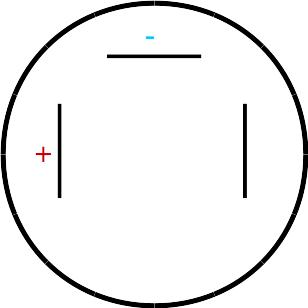
\includegraphics[width=0.2\textwidth]{pictures/hohlstecker_buchse.jpg}
	\caption{Pin-Layout Hohlstecker-Buchse \grqq HEBL 21\grqq }
	\label{fig21}
\end{figure}
\vspace{0.5cm} 

Die alten Litzen des Motors werden nun durch die neuen l"angeren Litzen ersetzt. Dabei m"ussen die rote Litze einmal durchtrennt und wie gehabt mit dem Stromschalter verbunden werden. \\
\\
Im Anschluss wird der Drucktaster mit den angel"oteten Litzen, von unten in das gro"se Loch der Platine (zwischen R2 und D2) gesteckt. Die Litzen f"uhrt man dazu ebenfalls von unten nach oben durch das Loch.
Die beiden Litzen (rot und schwarz) werden nun an den beiden L"ochern von SW1 von oben festgel"otet. Die Polung spielt hier keine Rolle.\\
Sobald der Drucktaster SW1 an der Platine festgel"otet wurde, k"onnen die auch die LEDs (D1-D4), die Hochlstecker-Buchse (J2) und der Motor (J3) festgel"otet werden. Hierbei muss auf die Polung der LEDs, der Hohlstecker-Buchse und des Motors geachtetet werden - die schwarzen Litzen (Minus-Pol) m"ussen in die L"ocher mit den quadratischen Kontakten. Im Fall einer Verpolung kann es zu Sch"aden an der Platine, zu nicht funktionierenden LEDs oder einen Motor der in die falsche Richtung dreht kommen.
In der Abbildung ~\ref{fig22} ist die fertig gel"otete Platine zu erkennen (ohen Motor).

\vspace{1cm}
\begin{figure}[!ht]
	\centering
  	\subfigure[Oberseite]{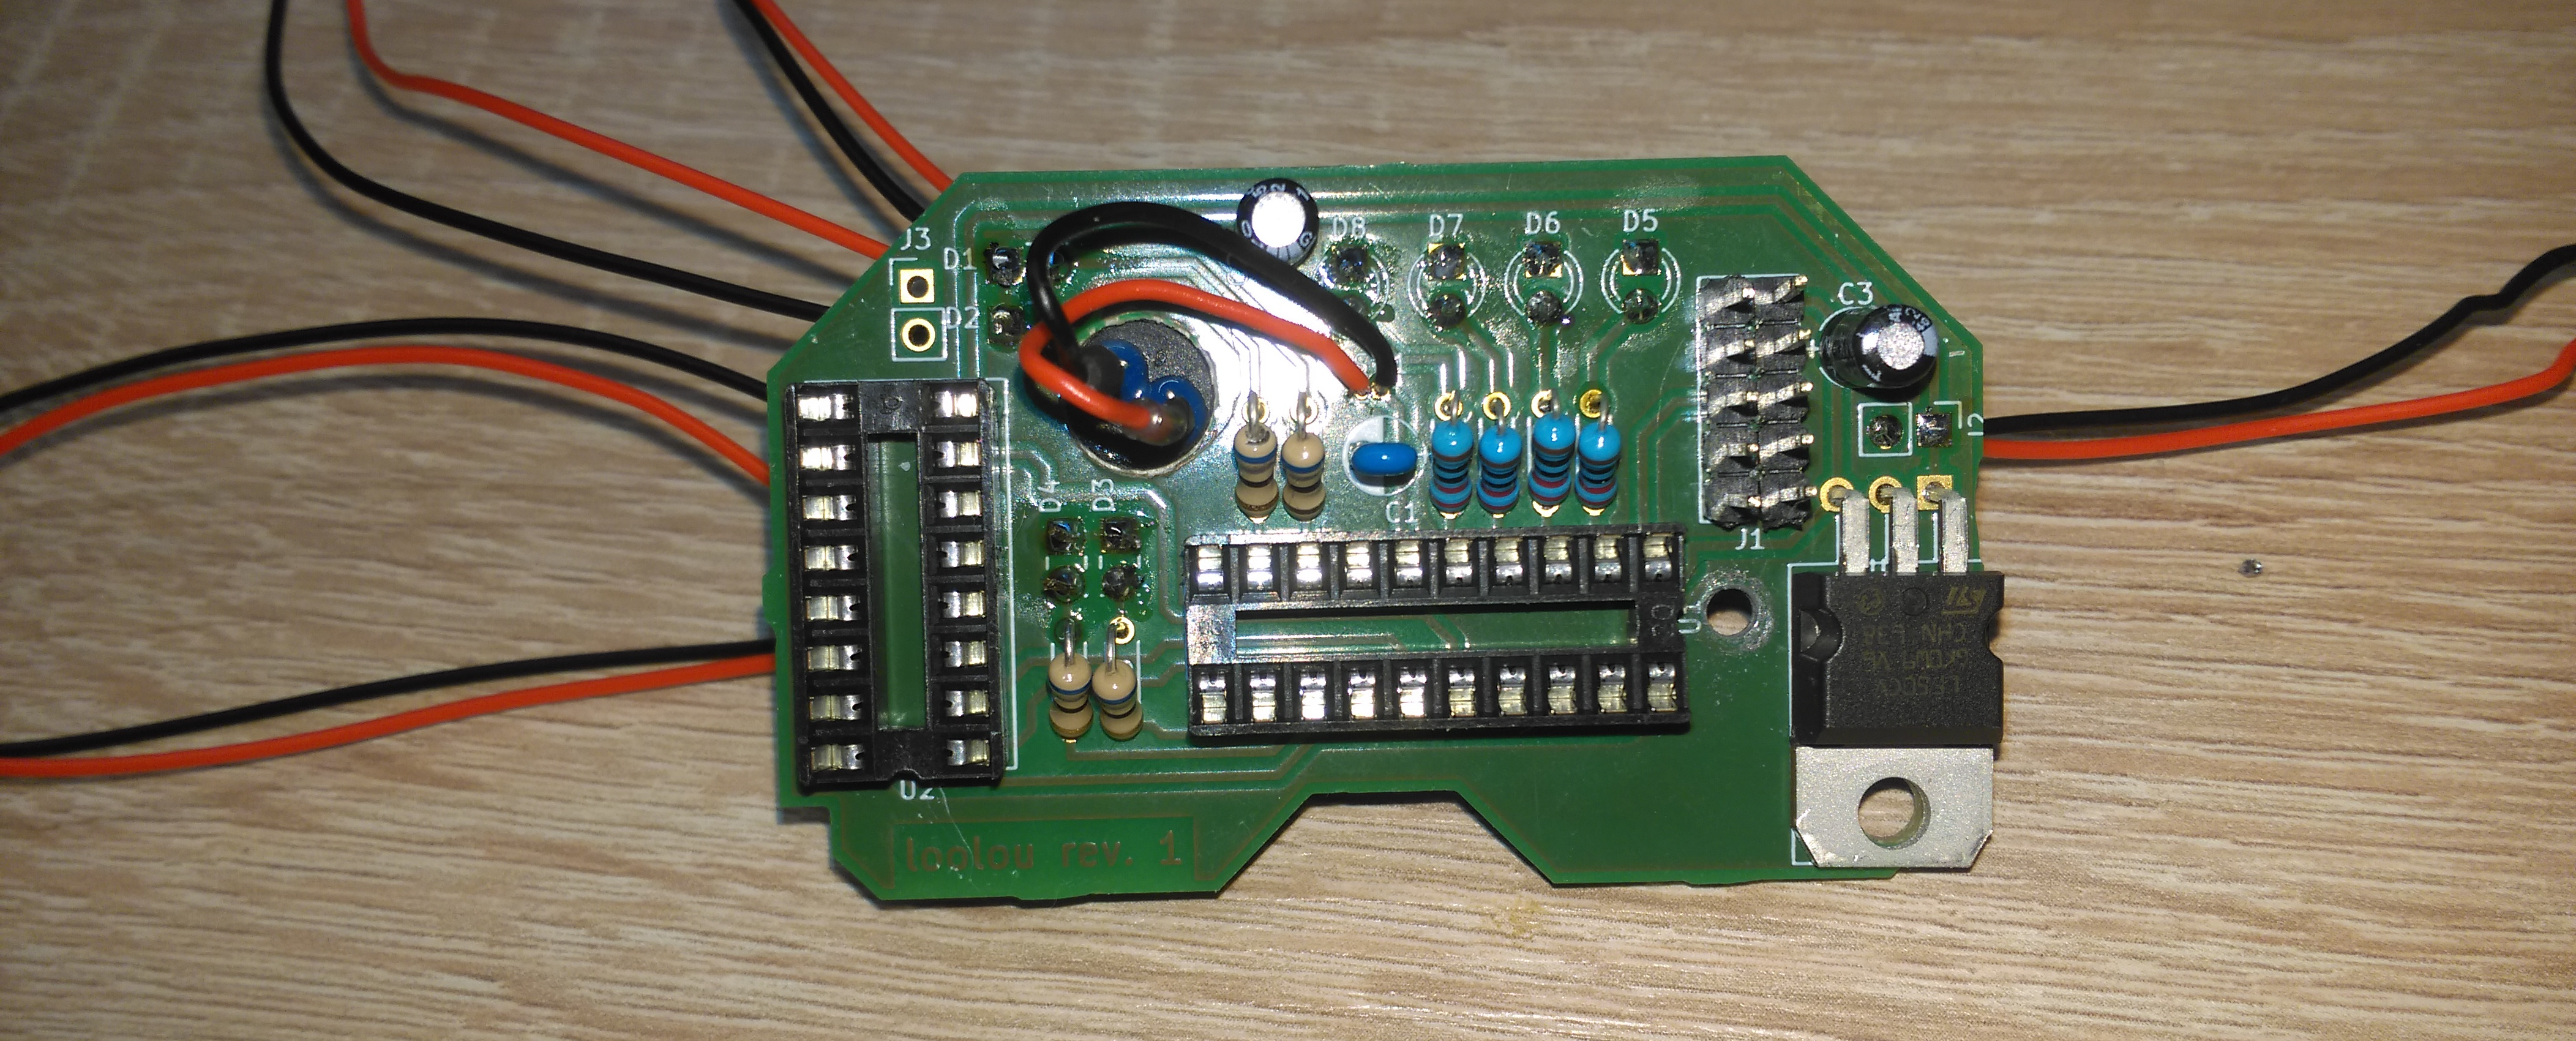
\includegraphics[width=0.7\textwidth]{pictures/loolou_021.jpg}}
	\subfigure[Unterseite]{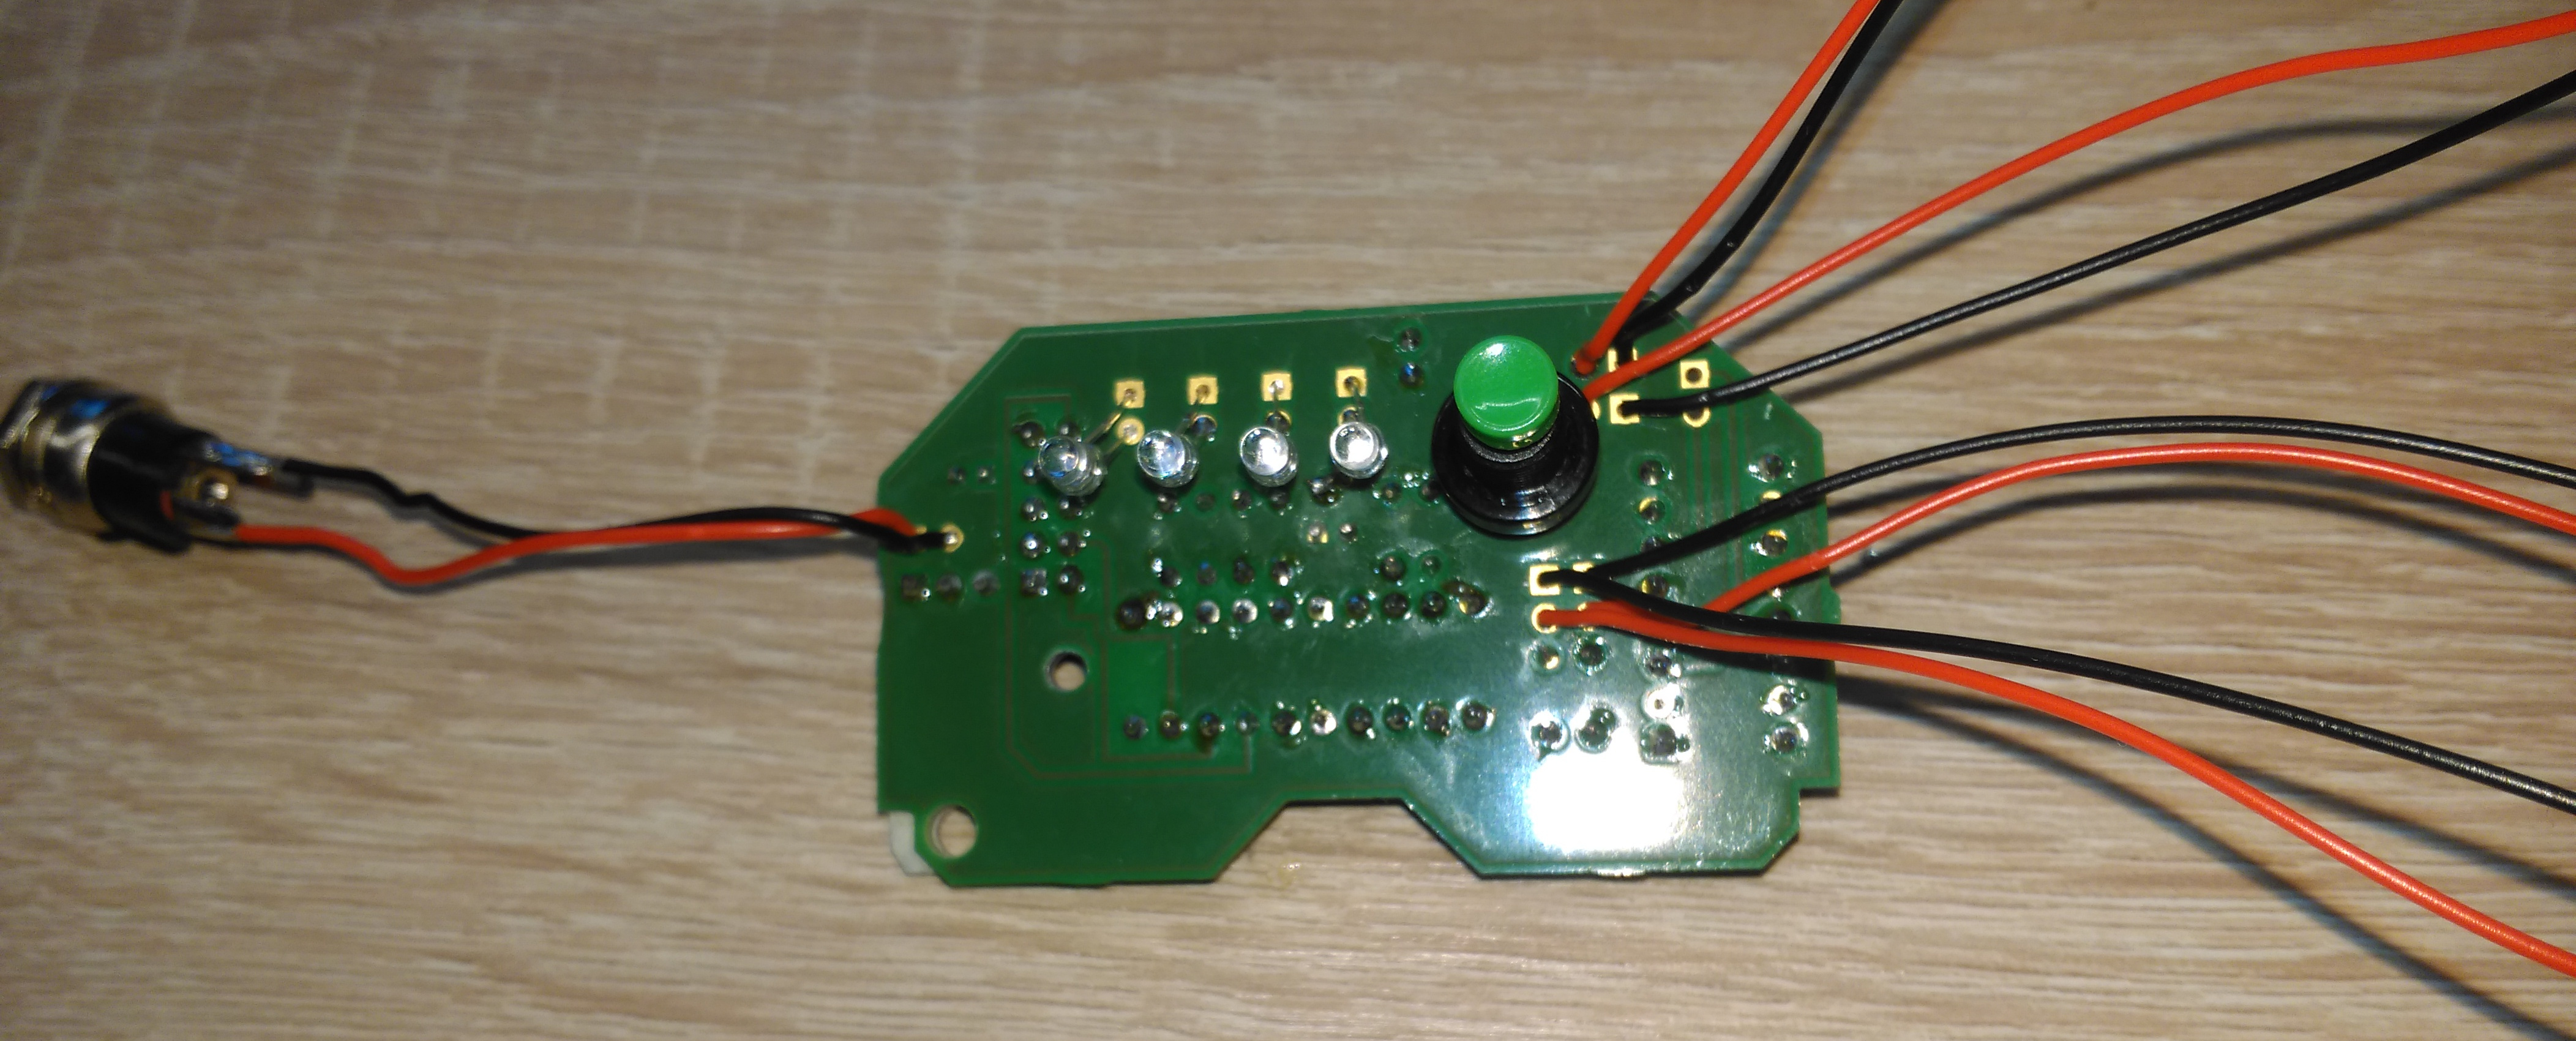
\includegraphics[width=0.7\textwidth]{pictures/loolou_022.jpg}}
	\caption{Platine mit allen Bauteilen (ohne Motor)}
	\label{fig22}
	%\label{fig23}
\end{figure}
\vspace{0.5cm}

Nun sollte die Platine nochmals mit dem Durchgangspr"ufer, auf kalte L"otstellen und verpolte Bauteile, "uberpr"uft werden. Ist hier kein Fehler zu finden, dann kann zum testen das Netzteil angeschlossen werden. Wird der Festspannungsregler schnell sehr hei"s dann deutet dies auf einen Kurzschluss oder eine Verpolung hin. Weiterhin sollte zwischen den Pins 1 und 2 des Festspannungsregler eine Spannung von 9 Volt und zwischen Pin 2 und Pin 3 ein Spannung von 5V anliegen. \\

Im Anschluss kann der Attiny2313 und der Treiberbaustein (L293D) auf die Sockel gesteckt werden. Die hablrunden Einkerbungen m"ussen daf"ur "uber den wei"sen halbrunden Kreisen des Zeichnung (bei U1 und U2) liegen. \\

Steckt man nun wieder das Netzteil ein, dann sollten die LEDs D1 bis D5 abwechselnd und die LED D8 dauerhaft leuchten. Der Motor kann "uber den Stromschalter, zwischen J3 und Motor, an bzw. ausgeschalten werden.
Durch den Druck auf den Drucktaster (SW1) k"onnen die LEDs D5 bis D7 getestet werden. \\
\\
Ist bisher kein Fehler erkennbar, dann kann man die Platine ausschalten und zur Seite legen.
 

\newpage
\subsection{Zusammenbau}

Nun werden alle Komponenten wieder zusammengebaut.
Beginnen muss man beim Zusammenbau mit dem Getriebe. Dazu nimmt man das blaue Zahnrad und steckt es in das gro"se Loch des Oberteils der Spielbasis. Anschlie"send m"ussen die wei"sen Zahnr"ader eingesetzt werden. Nachdem diese eingsetzt wurden, wird die Platine in das Oberteil geschraubt, dazu f"uhrt man die Litzen der LEDs, des Motors und der Hohlstecker-Buchse an der linken bzw. rechten Seite heraus. Der Stromschalter des Motors und der Motor selbst werden wieder in die Unterseite der Spielbasis eingesetzt bzw. festgeschraubt. Wie dies am Ende aussehen muss zeigt die Abbildung ~\ref{fig23}.

\vspace{0.5cm}
\begin{figure}[!ht]
	\centering
  	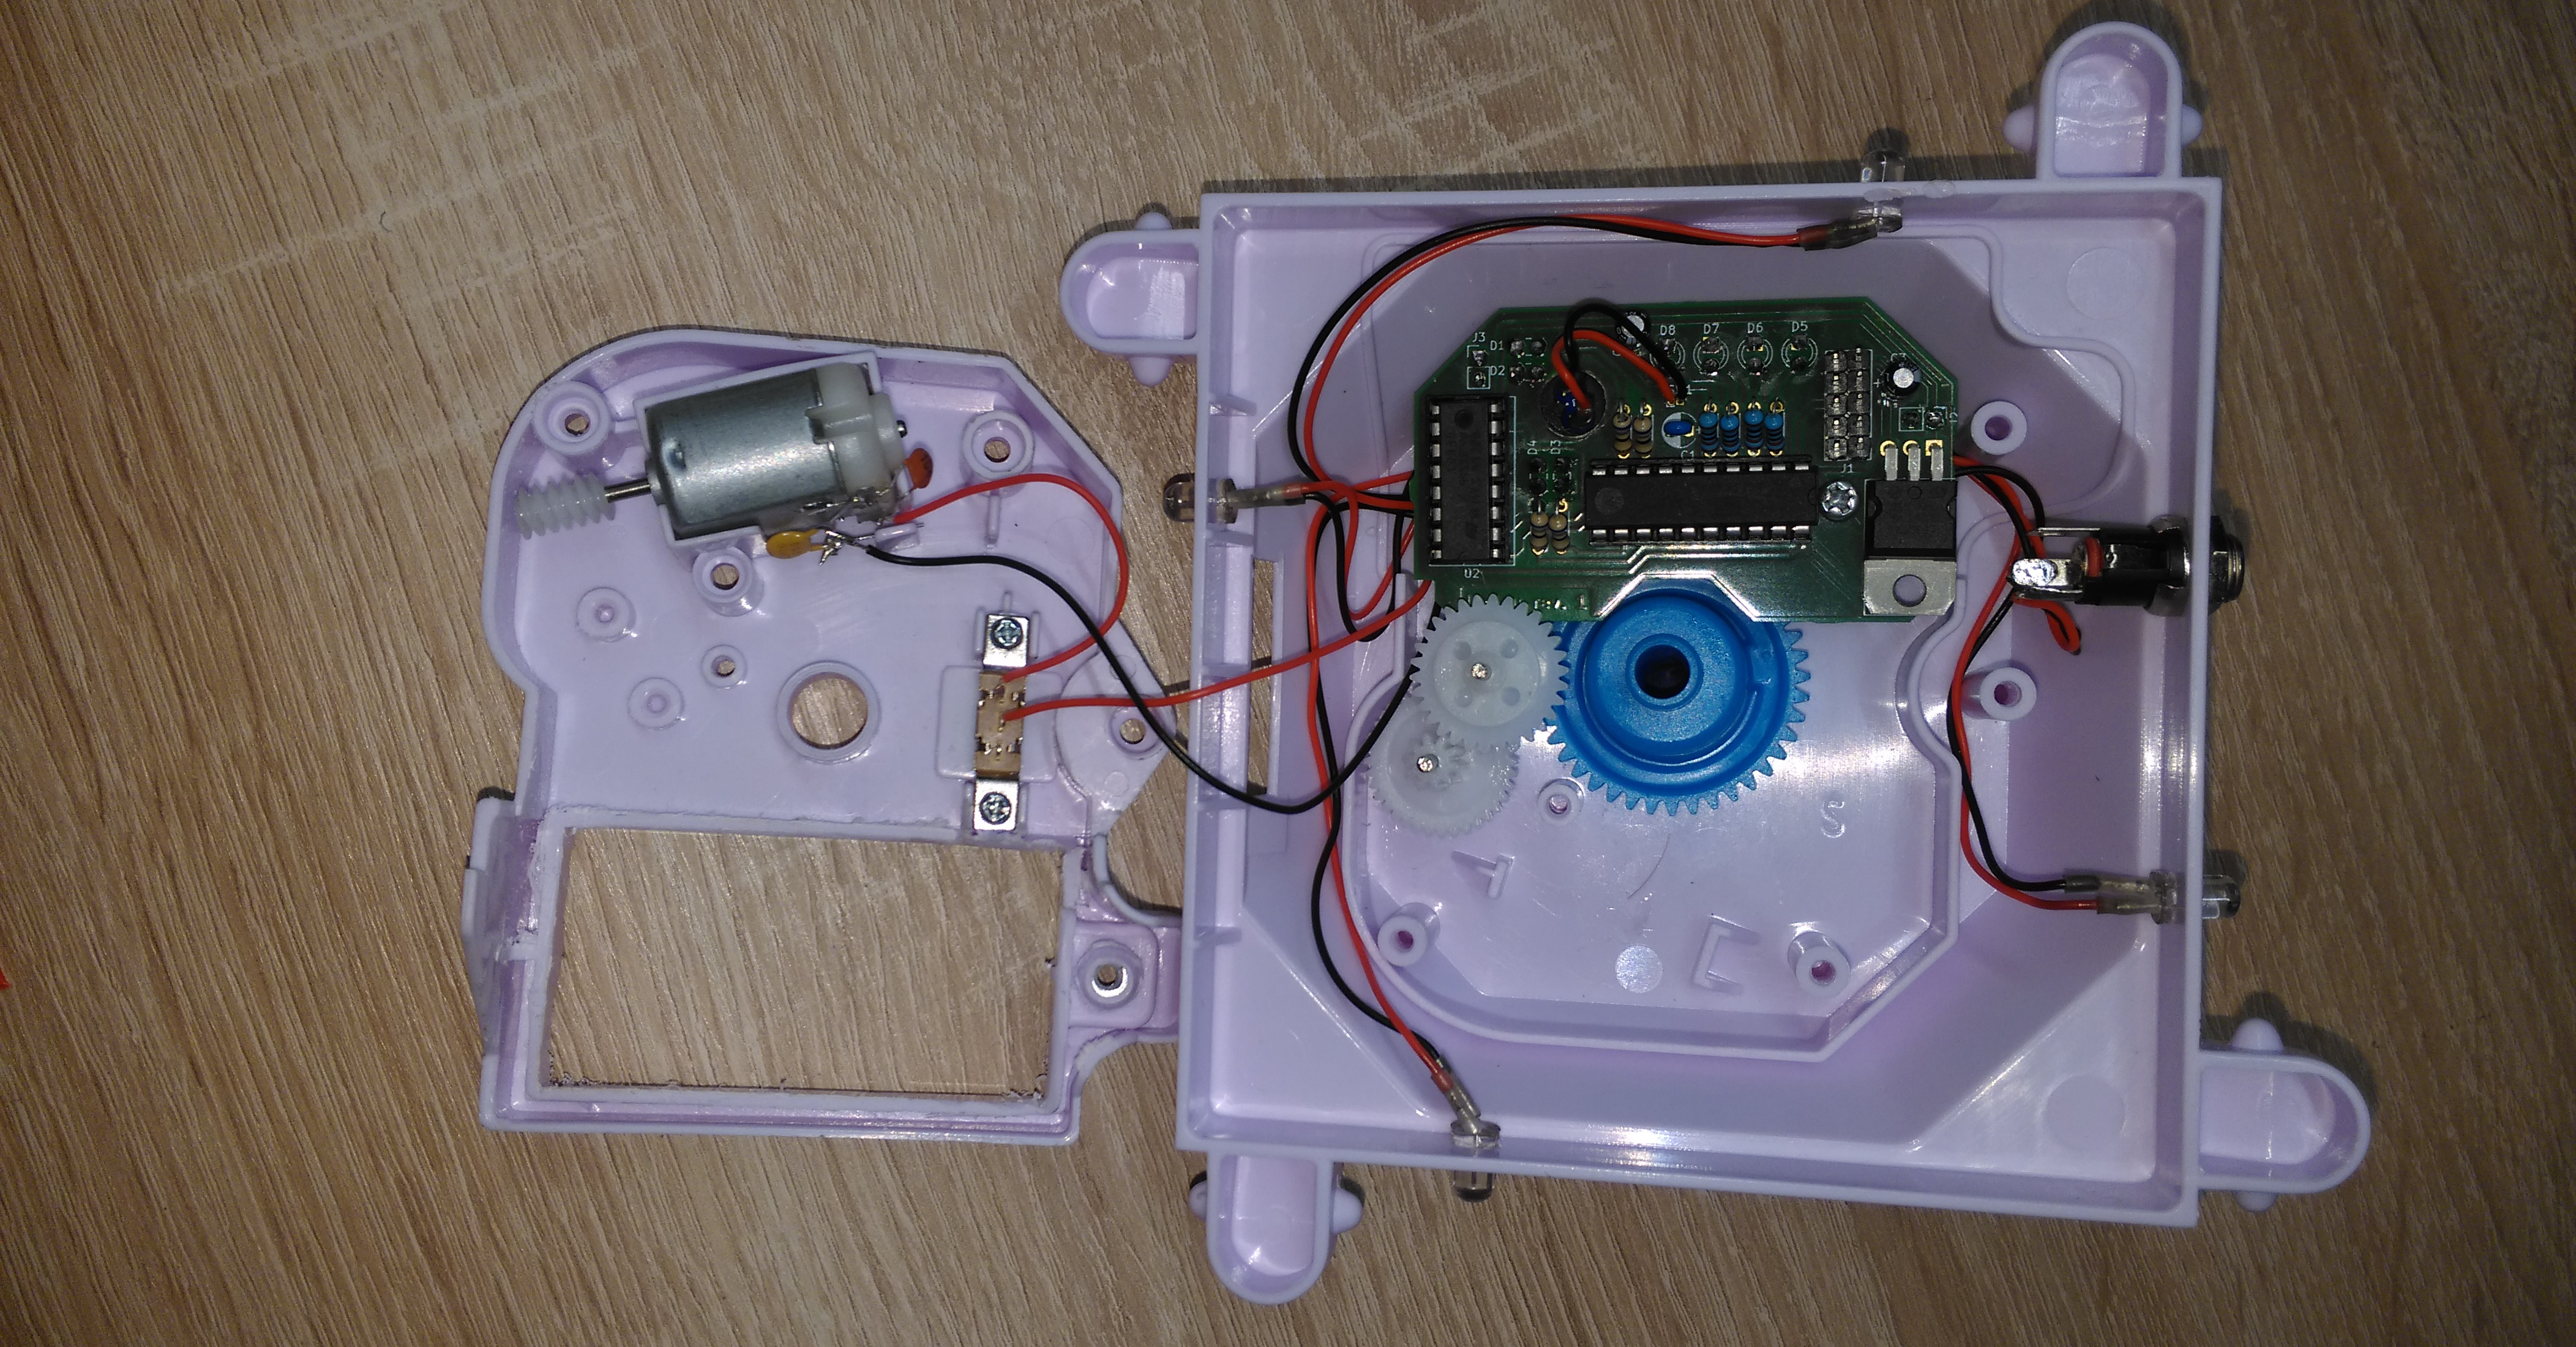
\includegraphics[width=0.7\textwidth]{pictures/loolou_023.jpg}
	\caption{Spielbasis mit eingesetzter Platine}
	\label{fig23}
\end{figure}
\vspace{0.5cm} 

Im Anschluss wird die Unterseite auf die Oberseite gesetzt und die 5 Schrauben der Spielbasis wieder fetsgeschraubt. Nun sollte man pr"ufen, ob die Spielbasis wieder richtig schlie"st. Sollte beim Vorbereiten der Spielbasis nicht sauber gearbeitet worden sein, dann muss hier nochmals nachgearbeitet werden. Die Spielbasis darf keine Erhebungen aufwei"sen, ansonsten steht die Spielbasis nicht sicher oder der Arm des Looping Louie kann nicht rivhtig arritiert werden.
Die Abbildung ~\ref{fig24} zeigt die wieder zusammengebaute Spielbasis ohne Batteriefachabdeckung.

\vspace{0.5cm}
\begin{figure}[!ht]
	\centering
  	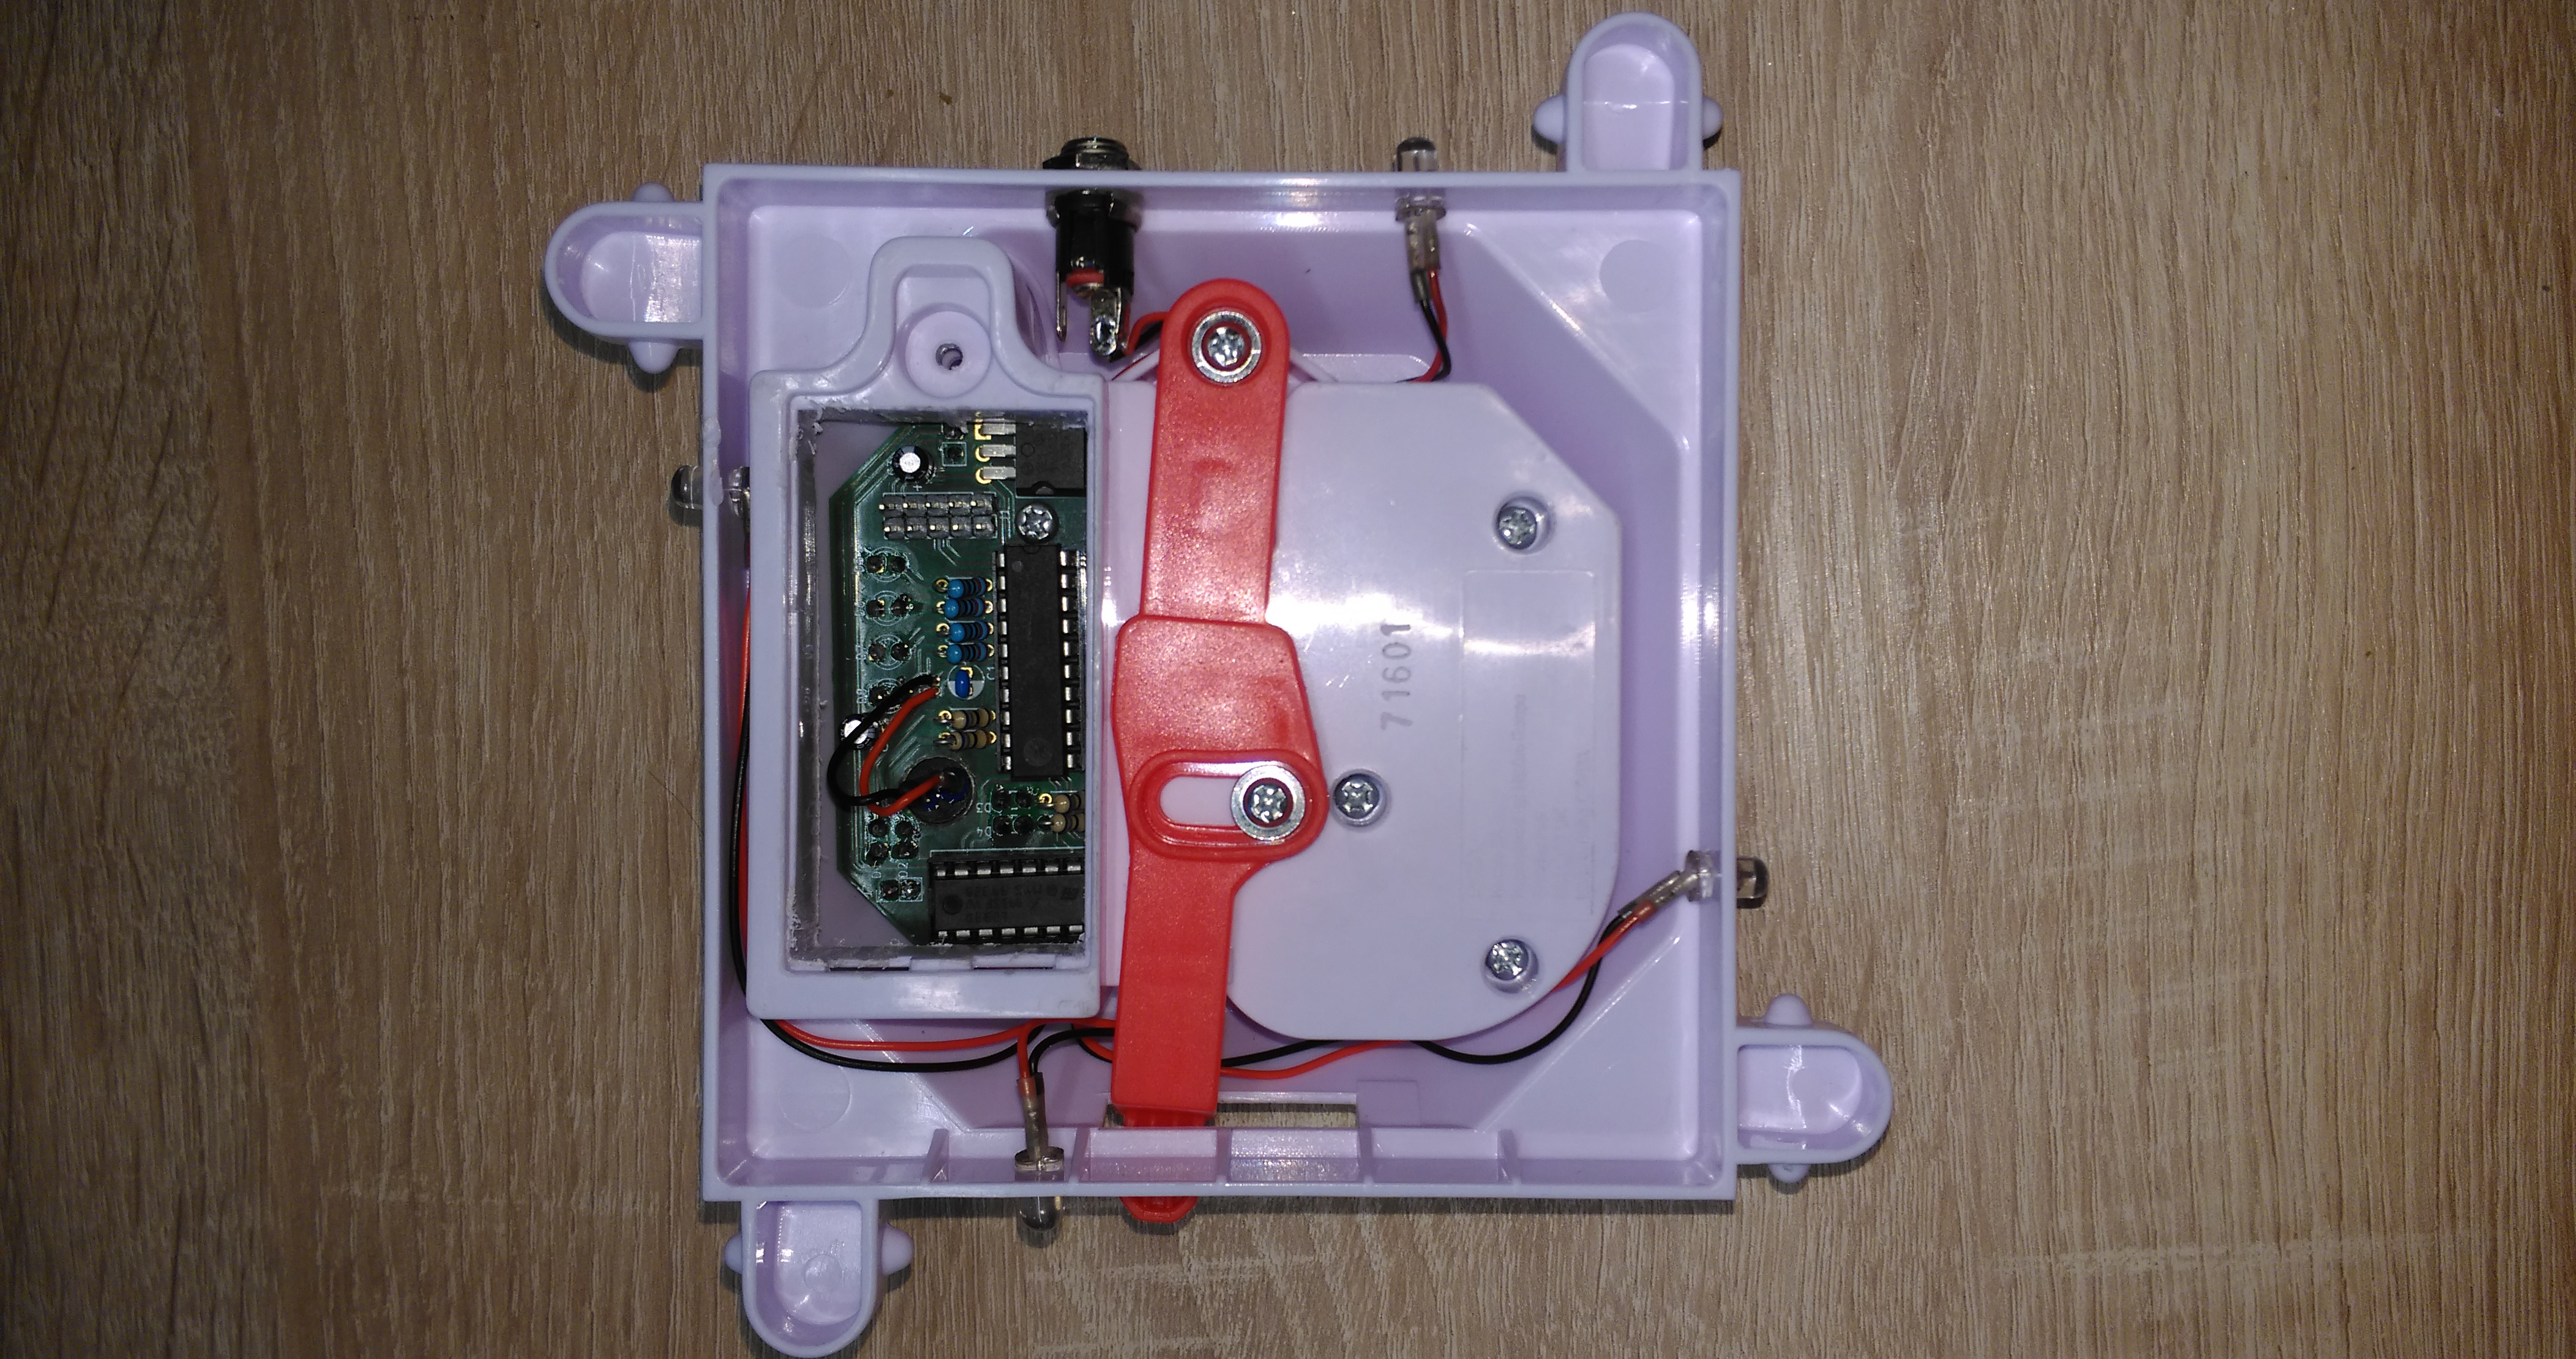
\includegraphics[width=0.7\textwidth]{pictures/loolou_024.jpg}
	\caption{Zusammengebaute Spielbasis ohen Batteriefachabdeckung}
	\label{fig24}
\end{figure}
\vspace{0.5cm} 

In der folgenden Abbildung (Abbildung ~\ref{fig25}) ist die geschlossene Spielbasis von oben und unten zu sehen.

\vspace{1cm}
\begin{figure}[!ht]
	\centering
  	\subfigure[Oberseite]{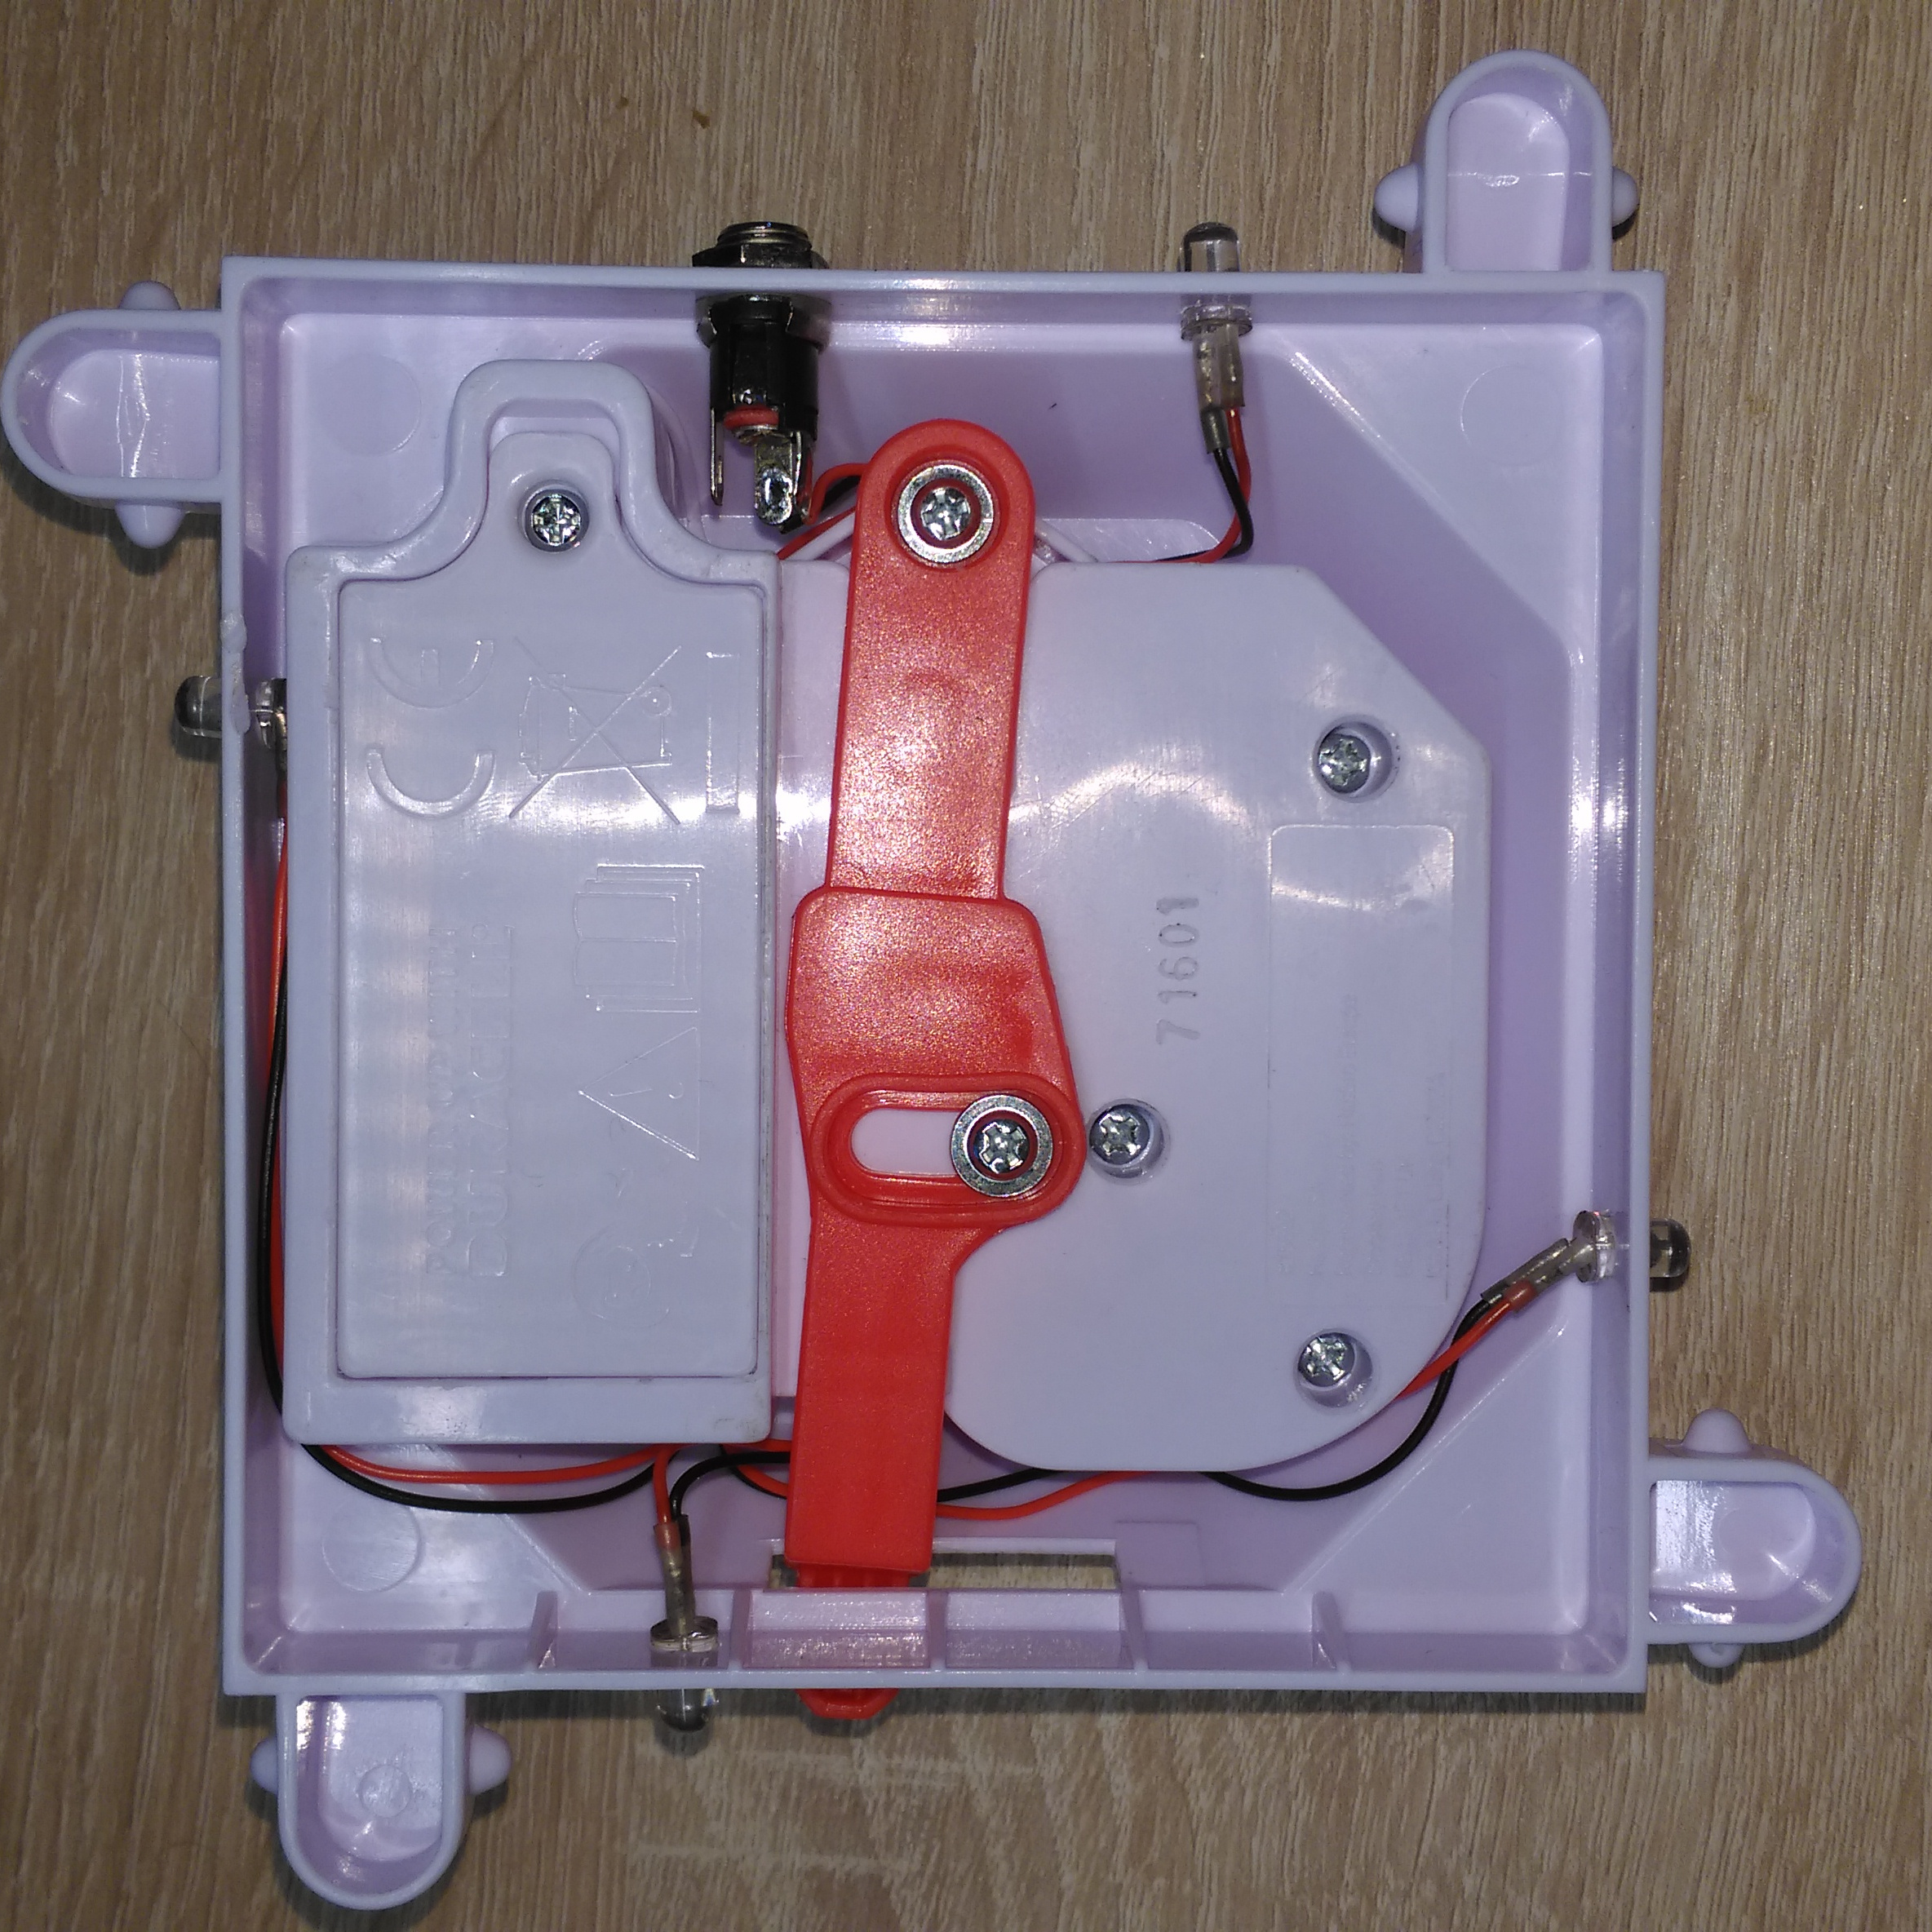
\includegraphics[width=0.49\textwidth]{pictures/loolou_025.jpg}}
	\subfigure[Unterseite]{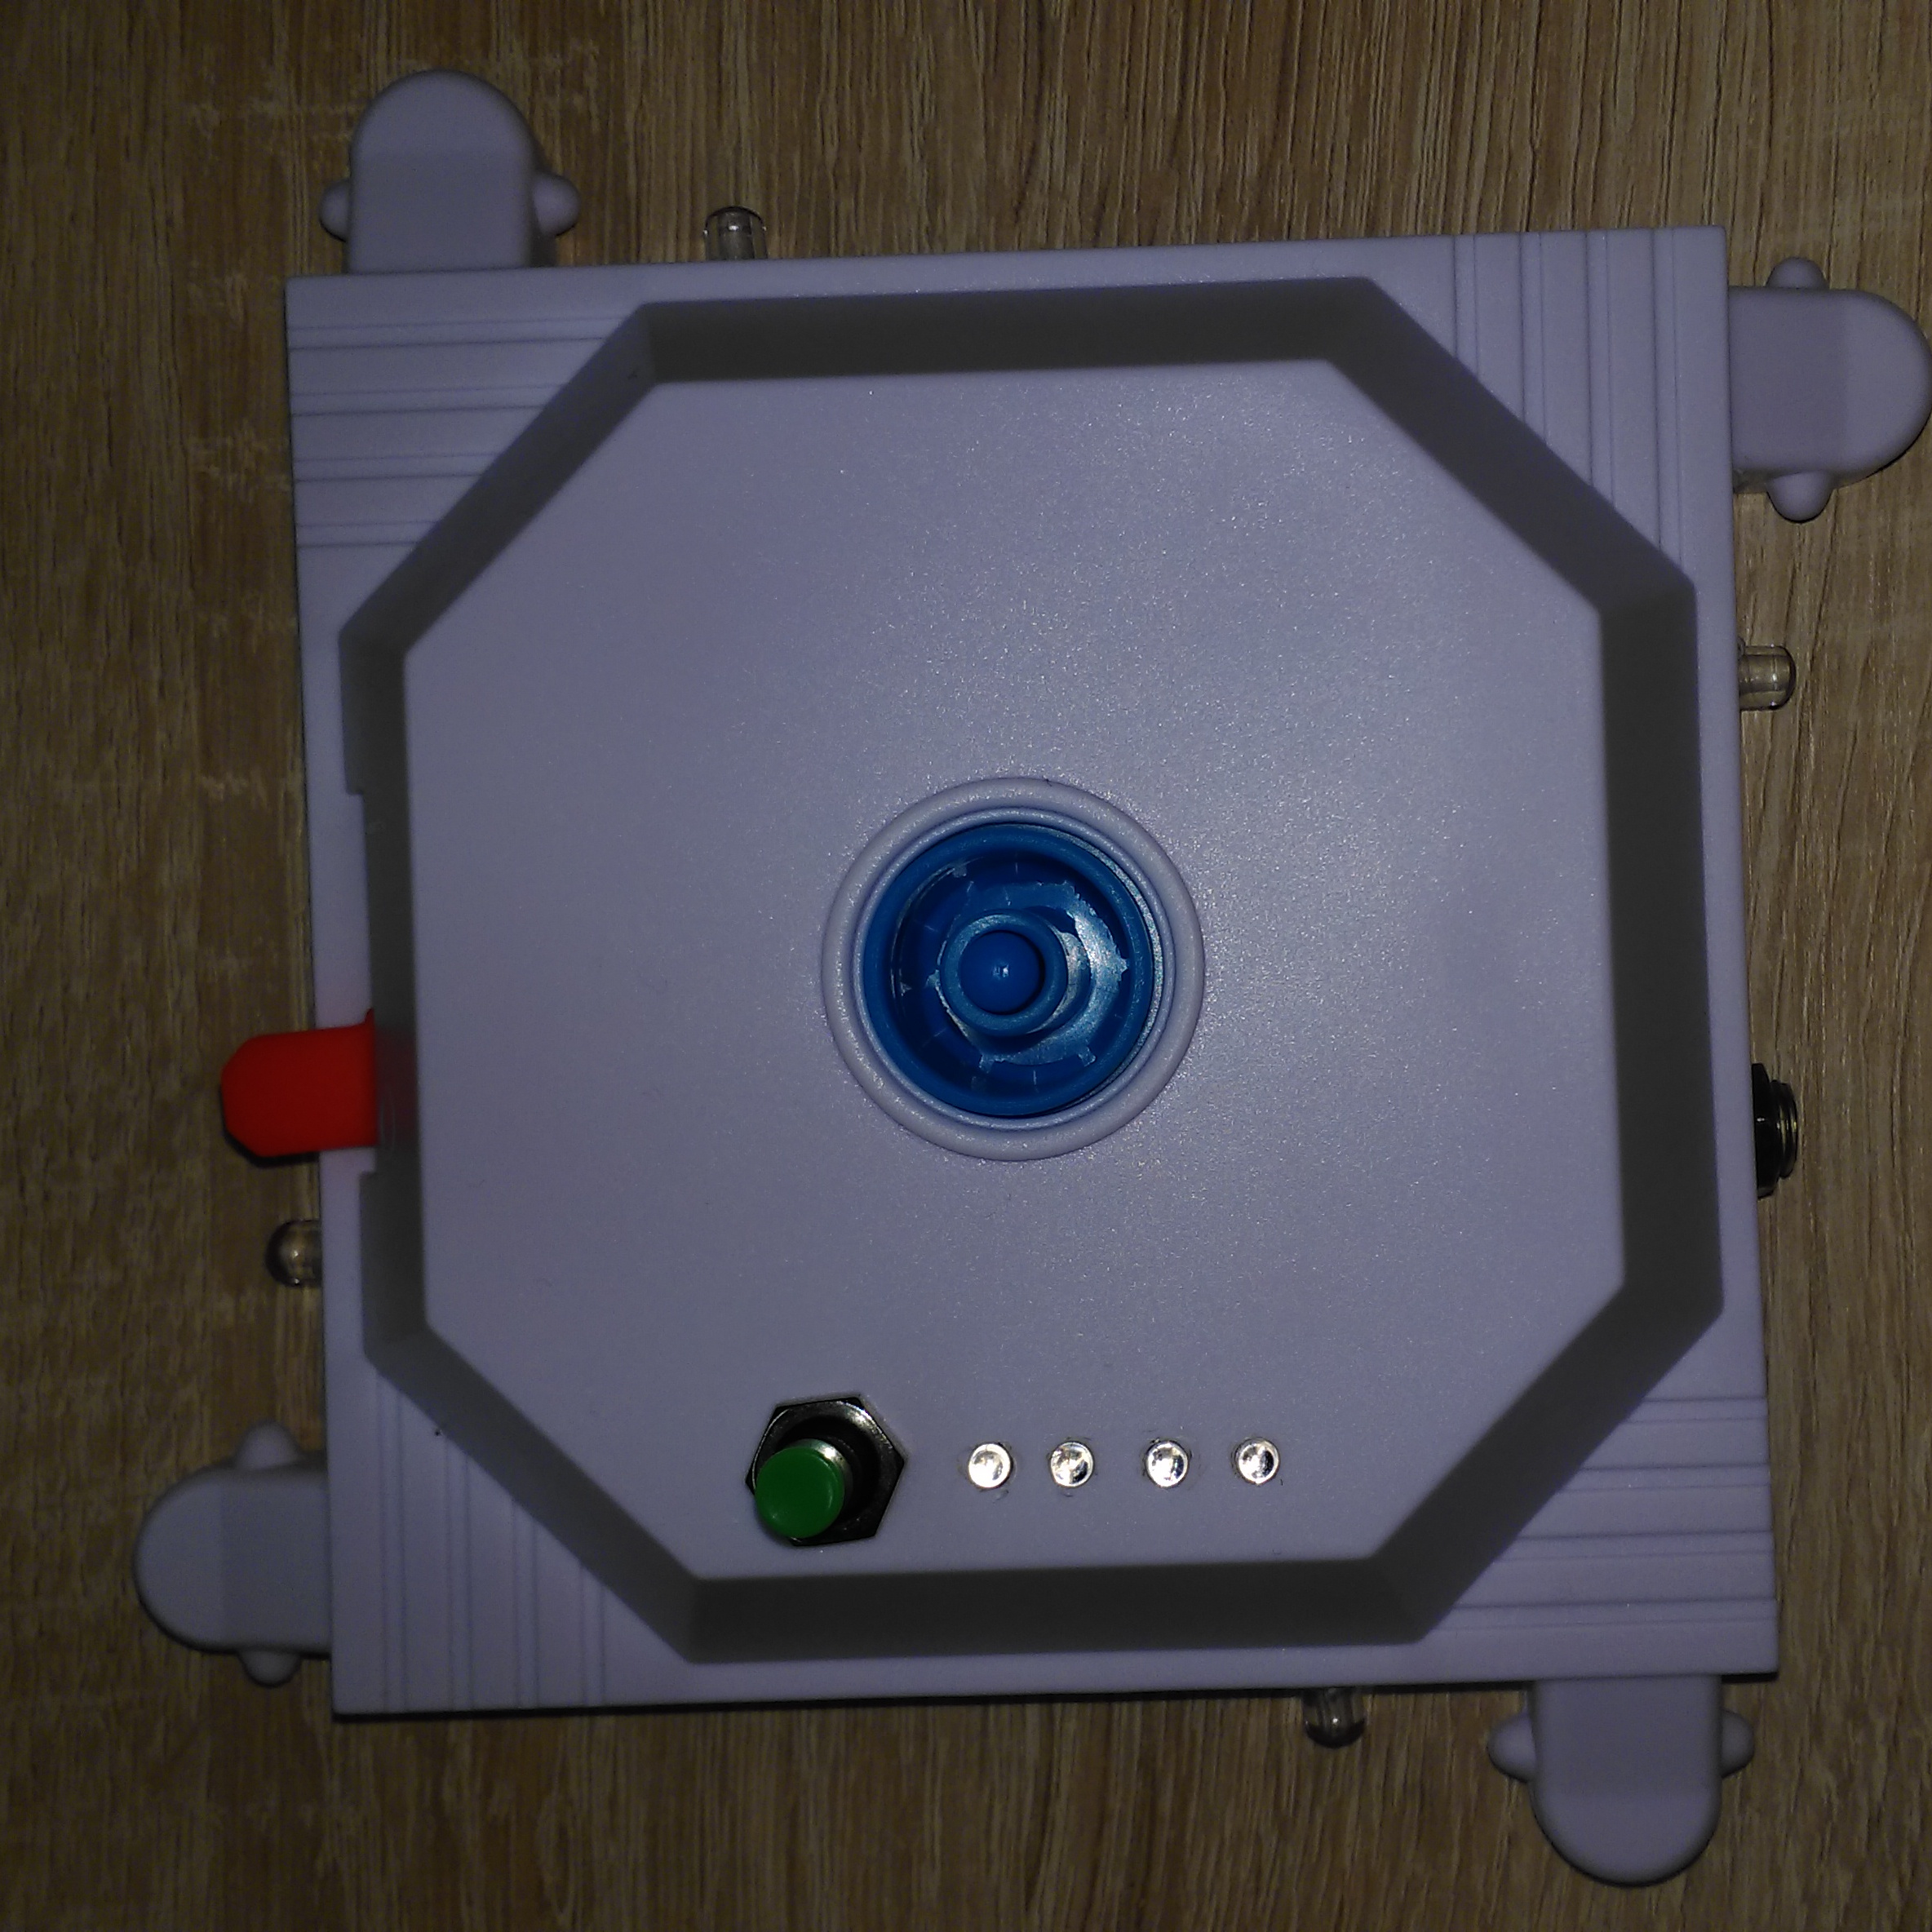
\includegraphics[width=0.49\textwidth]{pictures/loolou_026.jpg}}
	\caption{Platine mit allen Bauteilen}
	\label{fig25}
	%\label{fig23}
\end{figure}
\vspace{0.5cm}









